\documentclass[12pt,a4paper]{article}
\renewcommand{\baselinestretch}{1.5} 
\usepackage[utf8]{inputenc}
\usepackage{amsmath}
\usepackage{amsfonts}
\usepackage{amssymb}
\usepackage{titlesec}
\usepackage[edges]{forest}
\usepackage[parfill]{parskip}
\usepackage{listings}
\usepackage{natbib}
\usepackage{url}
\usepackage{multicol}
\usepackage{array}
\usepackage{float}
\usepackage{geometry}%
% \usepackage[twoside,bindingoffset=1cm]{geometry}%

\geometry{a4paper, left=25.4mm, right=25.4mm, top=31.7mm, bottom=31.7mm, asymmetric}

\usepackage{graphicx}
\graphicspath{ {screenshots/} }

\setcounter{secnumdepth}{4}

\usepackage{color}

\definecolor{codegreen}{rgb}{0,0.6,0}
\definecolor{codegray}{rgb}{0.5,0.5,0.5}
\definecolor{codepurple}{rgb}{0.58,0,0.82}
\definecolor{backcolour}{rgb}{0.95,0.95,0.92}

\definecolor{grayishblue}{RGB}{106, 123, 164}
\definecolor{pink}{RGB}{241, 96, 119}
\definecolor{orange}{RGB}{255, 145, 77}
\definecolor{yellow}{RGB}{221, 173, 37}
\definecolor{green}{RGB}{103, 187, 53}
\definecolor{cyan}{RGB}{0, 190, 192}
\definecolor{blue}{RGB}{58, 141, 236}

\lstdefinestyle{sqlStyle}{
    backgroundcolor=\color{backcolour},
    commentstyle=\color{codegreen},
    keywordstyle=\color{magenta},
    numberstyle=\tiny\color{codegray},
    stringstyle=\color{codepurple},
    basicstyle=\footnotesize,
    breakatwhitespace=false,
    breaklines=true,
    captionpos=b, 
    keepspaces=true,
    showspaces=false,                
    showstringspaces=false,
    showtabs=false,
    tabsize=4,
    showlines=true
}

\definecolor{textttColor}{rgb}{0.204, 0.286, 0.369}
\let\Oldtexttt\texttt
\renewcommand\texttt[1]{{\ttfamily\color{textttColor}#1}}

\def\hiddenparcommand{\par}
\newcommand\otherhiddenparcommand{\par\noindent}
\newcommand\hiddencommacommand{, }
\forestset{%
  declare keylist register={split here ids},% the list of nodes to split the tree at
  split here ids={},
  declare keylist register={split here interjects},% the list of comments to put in between the tree parts
  split here interjects={},
  declare keylist={split here auto siblings}{},% a list to hold the siblings which need edge restoration
  declare toks register=split here toks,
  declare dimen register=tmpdima,
  tmpdima'=0pt,
  declare dimen register=tmpdimb,
  tmpdimb'=0pt,
  declare dimen register=tmpdimc,
  tmpdimc'=0pt,
  to widest/.style={
    tikz+={\path (\forestregister{tempdima}, \forestoption{y}) -- (\forestregister{tempdimb}, \forestoption{y});},
  },
  hide commas/.style={%
    split here toks+={\hiddencommacommand},
    split here toks+={#1},
  },
  split dir tree pre/.style={%
    label={[text=gray, anchor=north, font=\scriptsize]below:{[cont.]}{}},
  },
  split dir tree post/.style={%
    label={[font=\scriptsize, anchor=south, text=gray]above:{[cont.]}{}},
  },
  split dir tree auto post/.style={% this gets applied to the first node after a break
    split dir tree post,
    tempkeylistc'={},
    tmpdimb/.option=y,
    for nodewalk={
      while={
        > ORw2+d _+d < On=! & {y}{tmpdimb}{##2-##1} {\textheight-#1} {n'}{1}%
      }{
        next,
        tempkeylistc/.option=name
      }%
    }{},
    % save the list
    split here auto siblings/.register=tempkeylistc,
    tikz+/.process={% this tries to redraw the edges to the following siblings
      OOw2{edge}{id}%
      {%
        \path [##1] (!u.parent anchor |- .north) ++(\forestregister{folder indent},1ex) coordinate (before ##2) |- (.child anchor);
        \edef\tempa{\foresteoption{split here auto siblings}}
        \foreach \i in \tempa \path [##1] (before ##2) |- ({forest cs:\i.child anchor});
      }%
    },
  },
  split dir tree/.code={%
    \forestset{%
      draw tree stage/.style={
        for root'={
          tempdima/.min={%
            >OOw2+d{x}{min x}{####1+####2}%
          }{tree},
          tempdimb/.max={%
            >OOw2+d{x}{max x}{####1+####2}%
          }{tree},
          for tree={%
            to widest,
          },
        },
        tempcountb'=-1,
        do until={%
          strequal((split_here_ids),"")
        }{%
          tempkeylistb'={},
          tempkeylista'={},
          split register={split here ids}{,}{tempcounta,tempkeylistb+},
          split register={split here interjects}{,}{temptoksa,tempkeylista+},
          split here ids'/.register=tempkeylistb,
          split here interjects'/.register=tempkeylista,
        % Sašo Živanović: http://chat.stackexchange.com/transcript/message/28484520#28484520
         for nodewalk={%
           draw tree processing order/.style={%
             filter={tree}{> ORw+n< OR> & {id}{tempcounta}{########1+1}{id}{tempcountb}}%
           }%
         }{},
          for root'={draw tree},
          TeX/.process={Rw{temptoksa}{\otherhiddenparcommand ####1\hiddenparcommand}},
          tempcountb'/.register=tempcounta,
        },
        for nodewalk={%
          draw tree processing order/.style={%
            filter={tree}{>OR>{id}{tempcountb}}%
          }%
        }{},
        for root'={draw tree},
      },
    }%
  },
  split dir here auto/.style n args=2{%
    split dir tree pre,
    !next node.split dir tree auto post=#2,
    split here ids+/.option=id,
%     !next node.split resume here ids+/.option=id,
    split={#1}{,}{split here toks,hide commas},
    split here interjects/.register=split here toks,
  },
  split dir tree auto/.style={%
    split dir tree,
    before drawing tree={%
      tempdima/.max={y}{tree},
      tempdimc/.register=tempdima,
      tempdimd/.min={y}{tree},
      tempdima-/.register=tempdimd,
      tempdimb'=\textheight,
      tmpdima'=10ex,
      tmpdimc'=\pagetotal,
      while={%
        >RR>{tempdima}{tempdimb}%
      }{%
        for nodewalk={%
          root',
          until={%
            > ROw2+d RRw2+d > {tempdimc}{y}{##1-##2} {tmpdima}{tmpdimc}{\textheight-##2-##1}%
          }{next node},
          previous node,
          split dir here auto/.process={R_w2{tmpdima}{}{{##2}{##1}}},
          next node,
          tempdima/.option=y,
          tempdimc/.register=tempdima,
          tempdima-/.register=tempdimd,
          tmpdima'=15ex,
          tmpdimc'=0pt
        }{},
      },
    },
  },
}

\begin{document}
	\begin{titlepage}
	    % this is actually the cover
		\begin{center}
		
			B.Comp. Dissertation
			
			\vspace*{3.5cm}
			
			\fontsize{14pt}{14pt}\textbf {
			    Design and Implementation of a Location Based\\
                Data Tracking and Visualization Tool\\
                for Hardcore Traveller on iOS Platform\\
			}
			
			\vspace{4.5cm}
			
			By
			
			\vspace{0.5cm}
			
% 			Lei Mingyu
			Wang Jinghan
			
			\vfill
			
			Department of Computer Science\\
			School of Computing\\
			National University of Singapore\\
			2016/2017
			
		\end{center}
	\end{titlepage}
	
% 	\clearpage
% 	~
% 	\thispagestyle{empty}
% 	\clearpage
	
	\begin{titlepage}
		\begin{center}
		
			B.Comp. Dissertation
			
			\vspace*{1.5cm}
			
			\fontsize{14pt}{14pt}\textbf {
			    Design and Implementation of a Location Based\\
                Data Tracking and Visualization Tool\\
                for Hardcore Traveller on iOS Platform\\
			}
			
			\vspace{2.5cm}
			
			By
			
			\vspace{0.5cm}
			
% 			Lei Mingyu
            Wang Jinghan
			
			
			\vspace{2.5cm}
			
			Department of Computer Science\\
			School of Computing\\
			National University of Singapore\\
			2016/2017
			
		\end{center}
		
		\vfill
		
		\centering
		\begin{tabular}{ || p{3cm} p{5cm} || }
		    \hline
            % Project No:     &  H114470 \\
            Project No:     &  H114500 \\
            % Project No:     &  H114470, H114500 \\
            \hline
            \hline
            Supervisor:     &  Prof. Wong Lim Soon   \\
            \hline
            \hline
            Deliverables:   & Report: 1 Volume     \\
                            & Program: 1 ZIP File   \\
                            \hline
        \end{tabular}
        
        \vspace{1cm}
			
	\end{titlepage}
	
% 	\clearpage
% 	~
% 	\thispagestyle{empty}
% 	\clearpage
	
	
	\pagenumbering{roman}
    \section*{Abstract}
        \addcontentsline{toc}{section}{Abstract}
        Nowadays, mobile devices play an indispensable role in modern people's life. With the help of the technology, many of the daily tasks can be greatly facilitated. To be more specific, keeping a travel diary and writing journals are quite common among the hodophile. This project aims to provide them some assistance to keep the precious travel moments.
        
        Leifr is an iOS application based on MapKit framework and backed by SpatiaLite/Realm database. It allows the user to record, view, share and play back the travelling paths. This project is completed jointly by Lei Mingyu and Wang Jinghan in fulfilment for CP4101 B.Comp. Dissertation.\\~
        
        \textbf{Subject Descriptors:}
        
        \begin{tabular}{ p{1cm} p{1.5cm} p{10cm} }
            &D.1.5   &  Object-oriented Programming \\
            &D.2     &  Software Engineering    \\
            &H.2.8   &  Database Applications   \\
            &H.5.1   &  Multimedia Information Systems  \\
            &H.5.2   &  User Interfaces \\
        \end{tabular}
        
        \vspace{1cm}
        
        \textbf{Keywords:}
        
        \begin{tabular}{ p{1cm} p{12.8cm} }
            &iOS, mobile application, geographic data visualization, spatial database \\
        \end{tabular}
        
        \vspace{1cm}
        
        \textbf{Implementation Software and Hardware:}
        
        \begin{tabular}{ p{1cm} p{13cm} }
            &macOS 10.12 Sierra, Xcode 8.3, Instruments 8.3, Swift 3.1, iOS 10, Realm Browser 2.1.7,  iPhone, MacBook Pro \\
        \end{tabular}
        
    \clearpage
    
    
    \section*{Acknowledgment}
        \addcontentsline{toc}{section}{Acknowledgement}
         First of all, we want to give a special gratitude to our supervisor, Professor Wong Lim Soon. It his considerate suggestions, information, feedback and supervision in the past eight months that has helped us progress this far. We would also like to express our thanks to our main evaluator, Professor Wang Ye, for the feedback and comments he gave during the CA presentation. These feedback were really important for us to move forward in the correct direction.
         
         We would like to thank Professor Wong Lim Soon and Professor Wang Ye again, together with our moderators, Professor Chan Chee Yong and Professor Yap Hock Chuan, Roland. Thank you for the time and efforts you are about to put when grading our project, this report and presentations in the coming weeks.
         
         Another acknowledgement is to Professor Roger Zimmermann. Although we have not contacted or communicated with him directly in person, yet his inspiring research in the ``GeoVid'' project provided us a brand new vision into the integration of geo-location data and photos.
         
         Last but absolutely not least, we would like to express our sincerest appreciation to every professor who have taught us in the four-year undergraduate study in National University of Singapore, to every friend who helped and supported us in this project, and to everyone who is reading this report. It is your knowledge and interests that keep us always progressing, motivated and cheerful about what we do.
    \clearpage
    
    \addcontentsline{toc}{section}{List of Figures}
    \listoffigures
    
    \addcontentsline{toc}{section}{List of Tables}
    \listoftables
    \clearpage
	
	
	\tableofcontents


	\newpage


    \pagenumbering{arabic}
	\section{Introduction} % Lei
	    \subsection{Background}
	    \label{intro:background}
        \textit{``Well begun is half done''}, the ancient Greek philosopher Aristotle once wrote this in his work \textit{Politics}. Seventeen centuries passed, this famous proverb still applies in every single bits of people's life. As for travellers, the \textit{well begun} often comes from the thorough planning of their journey.
        
        One of the most effective way to plan the journey is by reading others' journals. Nowadays, travellers can easily find a huge amount of such information on travelling websites. Usually there are three categories of journals:
        \begin{itemize}
            \setlength\itemsep{-0.5em}
            \item the ones with lots of photos and sight recommendations
            \item the ones with lots of personal thoughts and understanding of different cultures
            \item the ones with detailed schedules and routes
        \end{itemize}
        
        We travelled a lot during the exchange period in Europe in 2016, our personal pain point is that when planning the journey, we can find tons of information of the first category listed above, but what we need most is actually the third one. After the travellers have some places in mind, the problem they need to solve is to organize them properly so that they have sufficient time spent in each of the places without wasting too much time travelling back and forth in between.
        
        There are various reasons why we can rarely find information of the third category. One possible cause might be the difficulties of keeping track of everything regarding the schedules and routes: as travellers, they may clearly remember the different sights they have visited, but seldom can they tell what time they left the hotel on the second day and how long did they spend on the bus from the hotel to the restaurant that they had lunch.
        
        To facilitate travellers to keep the information of their detailed travelling schedule, we come up with the idea of building an application using mobile phones with Global Positioning System (GPS) hardware to record and visualize the users' geo-location change within a period of time.
        
        \footnotesize
            Section \ref{intro:background} is written by Mingyu.
        \normalsize
	  
	    \subsection{Overview}
	    \label{intro:overview}
        Named after the Icelandic explorer Leifr Eiríksson, \textit{Leifr} is an iOS application to address the problem mentioned above. The core functions of this application includes:
        \begin{itemize}
            \setlength\itemsep{-0.5em}
            \item record a path of user's geo-location information (longitude, latitude and altitude) with the exact time that this information is recorded
            \item visualize the visited places on a map and color them in a ``heat map'' manner to indicate how frequent the user visits a specify location
            \item view/share/replay a recorded path
        \end{itemize}
        
        There are also some advanced features implemented:
        \begin{itemize}
            \setlength\itemsep{-0.5em}
            \item replay all the paths sequentially starting from a selected date
            \item estimate the location where a chosen photo is taken
            \item display the statistics about all the countries the user visited
        \end{itemize}
        
        Some of the extra features are planned to be implemented in the future. These will be discussed in the Section 5.3 \textit{Future Plans}.
        
        \footnotesize
            Section \ref{intro:overview} is written by Mingyu.
        \normalsize
        
        \subsection{Comparison to Existing Products}
        \label{intro:comparison}
        During the project ideation process, we studied some existing mobile applications that partially fulfil our requirements. In general, they can be categorized into three different types, and a typical example will be chosen from each of them and compared with our proposed applications.
        
        The three categories are:
        \begin{itemize}
            \setlength\itemsep{-0.5em}
            \item Map applications with the capability to keep track of the location history (e.g. Google Maps by Google, Inc.)
            \item Activity tracking app with the capability to share a path with others (e.g. Nike\texttt{+} Run Club by Nike, Inc.)
            \item Visited locations visualization app (e.g. Fog of World by Ollix)
        \end{itemize}
        
            \subsubsection{Google Maps}
            \label{intro:comparison:google-maps}
            Google Maps is probably one of the most popular and successful map application in the world, it provides a completed set of functionalities coming along with the map services like navigation, address finding and location sharing. In 2015, Google released a new feature in Google Maps called ``Your Timeline'' (\citet{GoogleMapsTimelineBlog}). It provides a way to track the user's location history as long as the user turn ``places you go'' on. The visualization result of the location history is shown in Figure \ref{fig:google-maps}.
            
            Google Maps effectively identifies the places the user visited recently, and predicts the mode of transportation based on the time spent in between. The result is like a normal navigation routes, all the critical places are identified and highlighted, then the paths in between are simply connecting those critical places. One strength of this timeline feature is the powerful map data support from Google; for example, in Figure \ref{fig:google-maps}, some of the photos are displayed for one of the place that the user visited, this definitely makes the history more informative. Nevertheless, this feature still lacks of some crucial functionalities we are looking for, like path sharing and full control of the start and end of recording a path. It's more like a auxiliary feature that provides some useful information feedback while the user is using the Google Maps app.
            
            \begin{figure}
                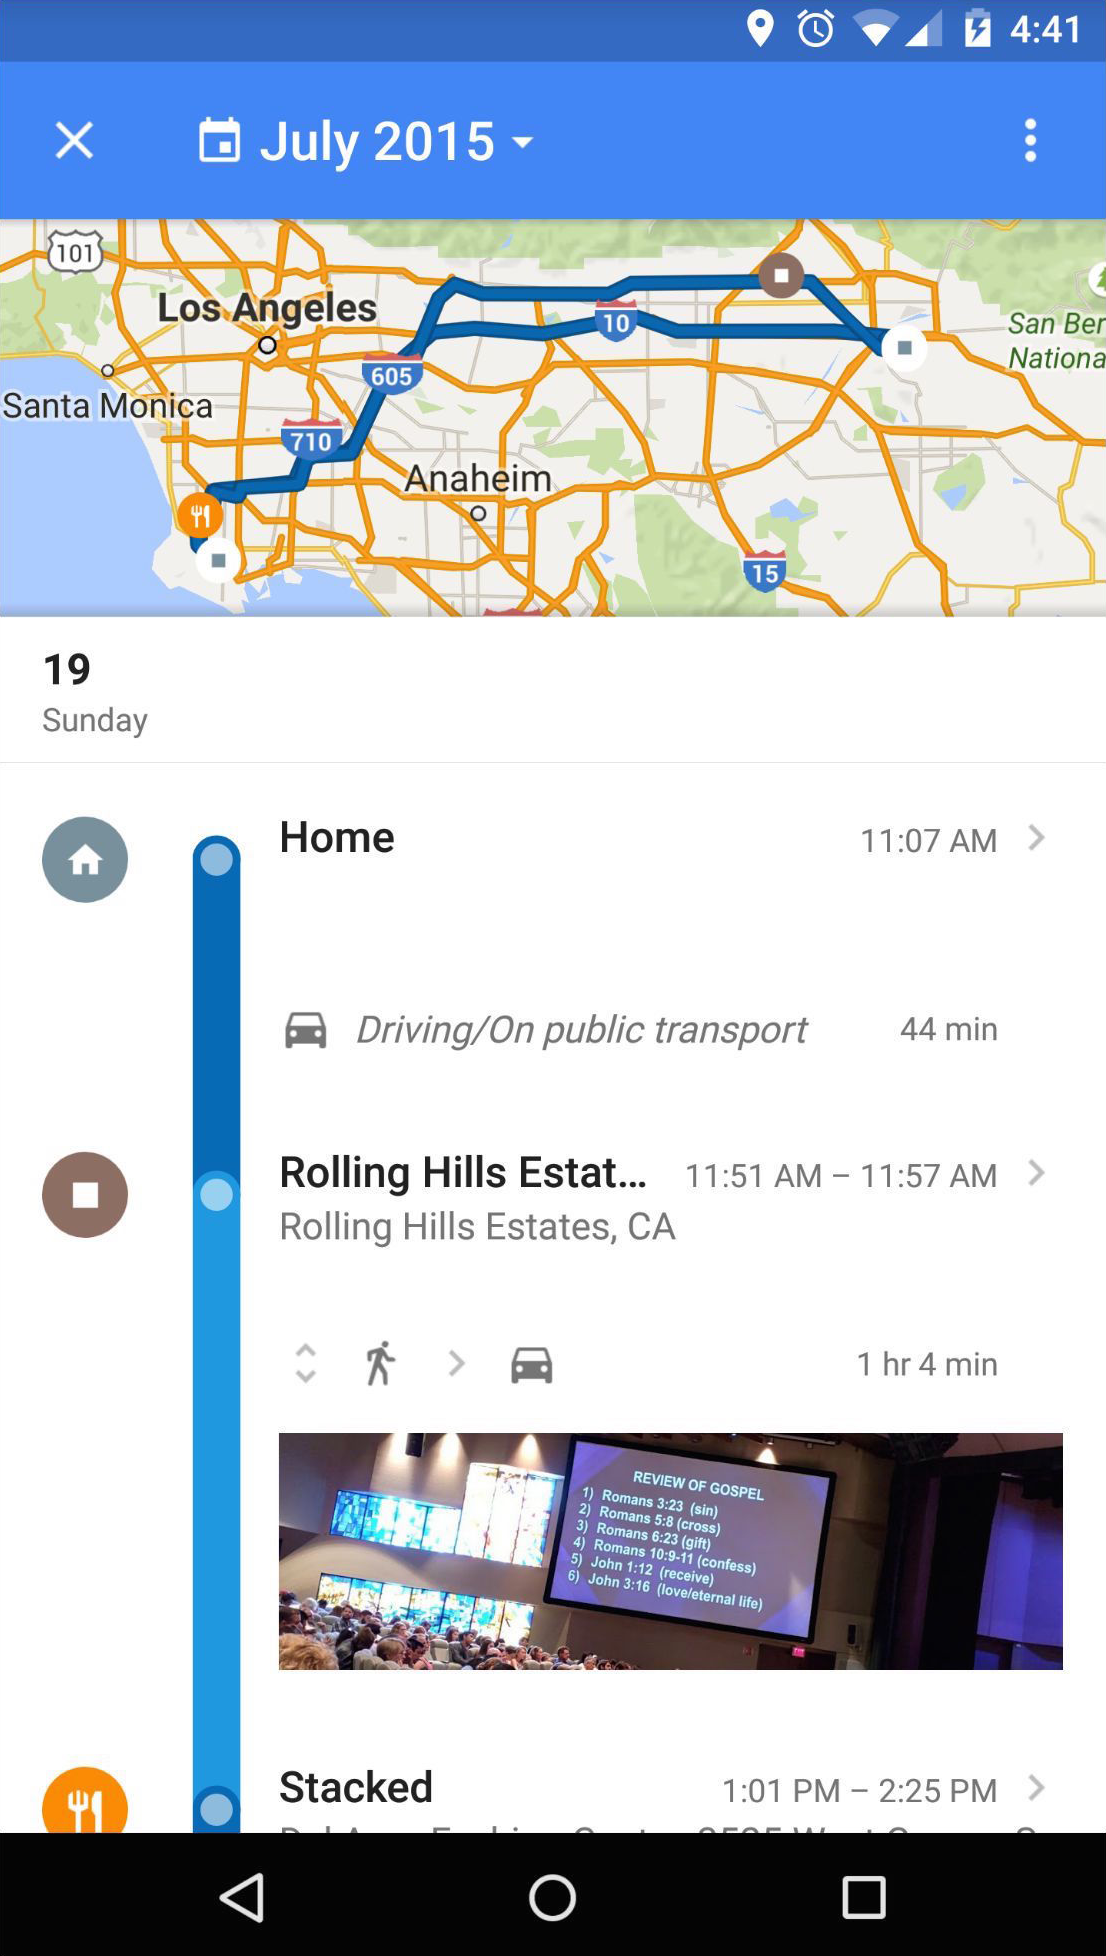
\includegraphics[width=.32\textwidth]{1-3-1}
                \centering
                \caption{Google Maps ``Your Timeline'' feature}
                \label{fig:google-maps}
            \end{figure}
            
            \subsubsection{Nike\texttt{+} Run Club}
            \label{intro:comparison:nike}
            Nike\texttt{+} Run Club is an application developed by Nike to assist the runners to manage their running plan, history and progress. The special feature we are particularly interested in is the GPS tracking and sharing.
            
            An example of the tracking result is shown in Figure \ref{fig:nike-plus-run-club}. Despite the fact that the app is using color hue as the visual variable to visualize the speed in different parts of the overall track (which is quantitative), it is a good visualization result as to mark the running path on the map. This result can be conveniently shared together with some statistics about the running experience like the duration and average pace. This is also what we want to achieve in the proposed application. Although Nike\texttt{+} Run Club meets the minimal core features we want to have for the traveller app, it also introduces lots of unnecessary details regarding the running statistics (after all it is a running app). Furthermore, it will be very unlikely to see some more advanced features for traveller like photo location finder to be integrated with this kind of app.
            
            \subsubsection{Fog of World}
            \label{intro:comparison:fow}
            Fog of World is gamified path history tracking tool that allows the user to clear the ``fog'' on the map while exploring the world. It clearly shows the path that the user visited and introduces lots of social element like leveling system, Apple Game Center integration and record sharing. Amongst the several existing apps mentioned in this section, Fog of World is the one closest to our proposed idea: designed for the travellers, support path history overview, cloud backup and import of past history. However, there is a key component from our proposal missing in this app: time. It will be much more interesting to add the time information on top of the geo-location data collected; for example, users can replay the path that they recorded a long time ago. This makes more sense when concerning about the travellers: date, time and even the season can be an important factor that they want to take into account when writing the journal and sharing with other travellers.
            
            \begin{figure}
                \centering
                \begin{minipage}{.5\textwidth}
                    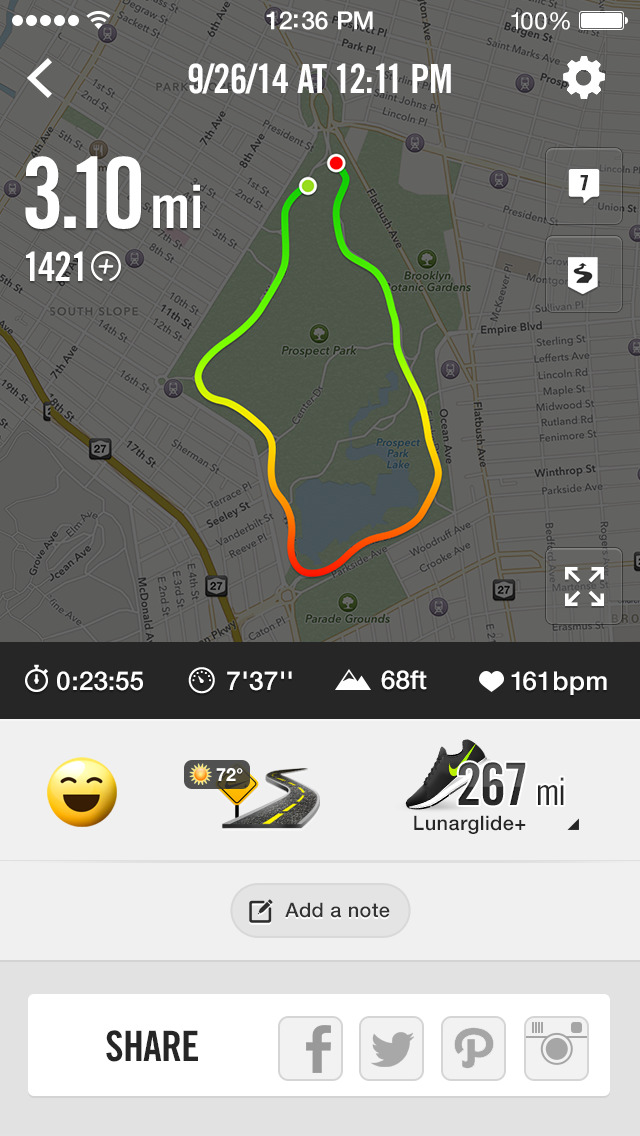
\includegraphics[width=0.66\textwidth]{1-3-2}
                    \centering
                    \caption{Nike\texttt{+} Run Club}
                    \label{fig:nike-plus-run-club}
                \end{minipage}%
                \begin{minipage}{.5\textwidth}
                    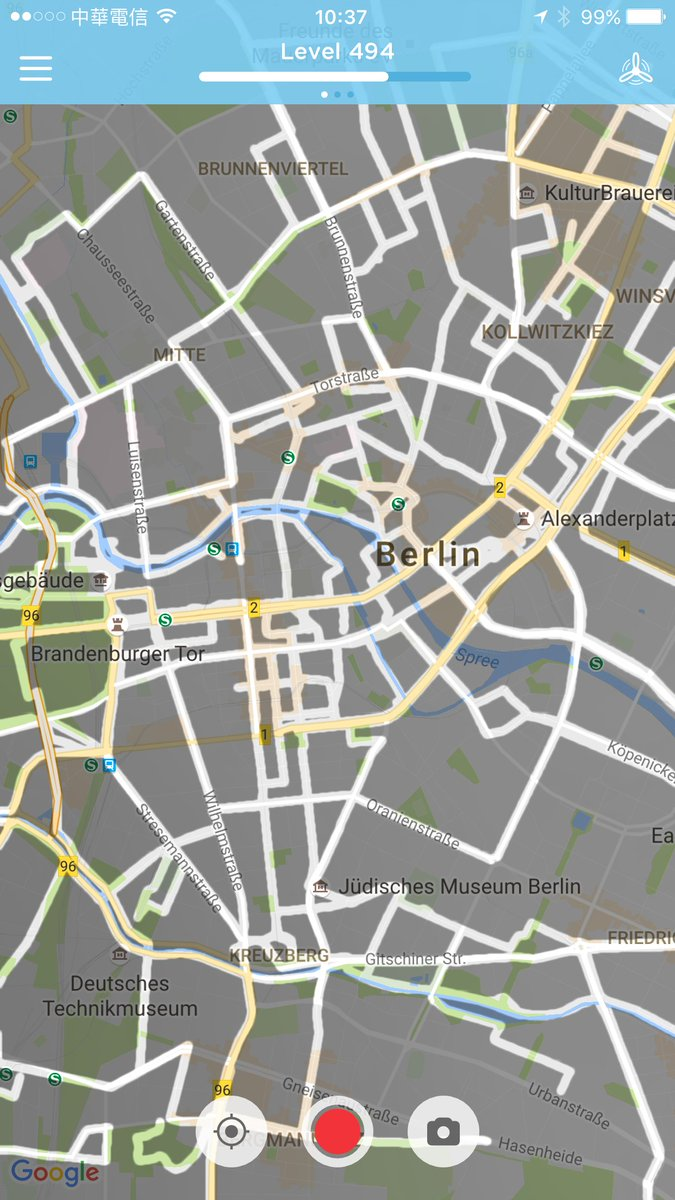
\includegraphics[width=0.66\textwidth]{1-3-3}
                    \centering
                    \caption{Fog of World}
                    \label{fig:fog-of-world}
                \end{minipage}
            \end{figure}
        
        \footnotesize
            Section \ref{intro:comparison} is written by Mingyu.
        \normalsize
    
    \clearpage
    
    
    \section{Use Cases and Demonstration}
        \subsection{View Aggregated Records} % Wang
            \label{sec:view-aggregated-records}
            \begin{figure}[H]
                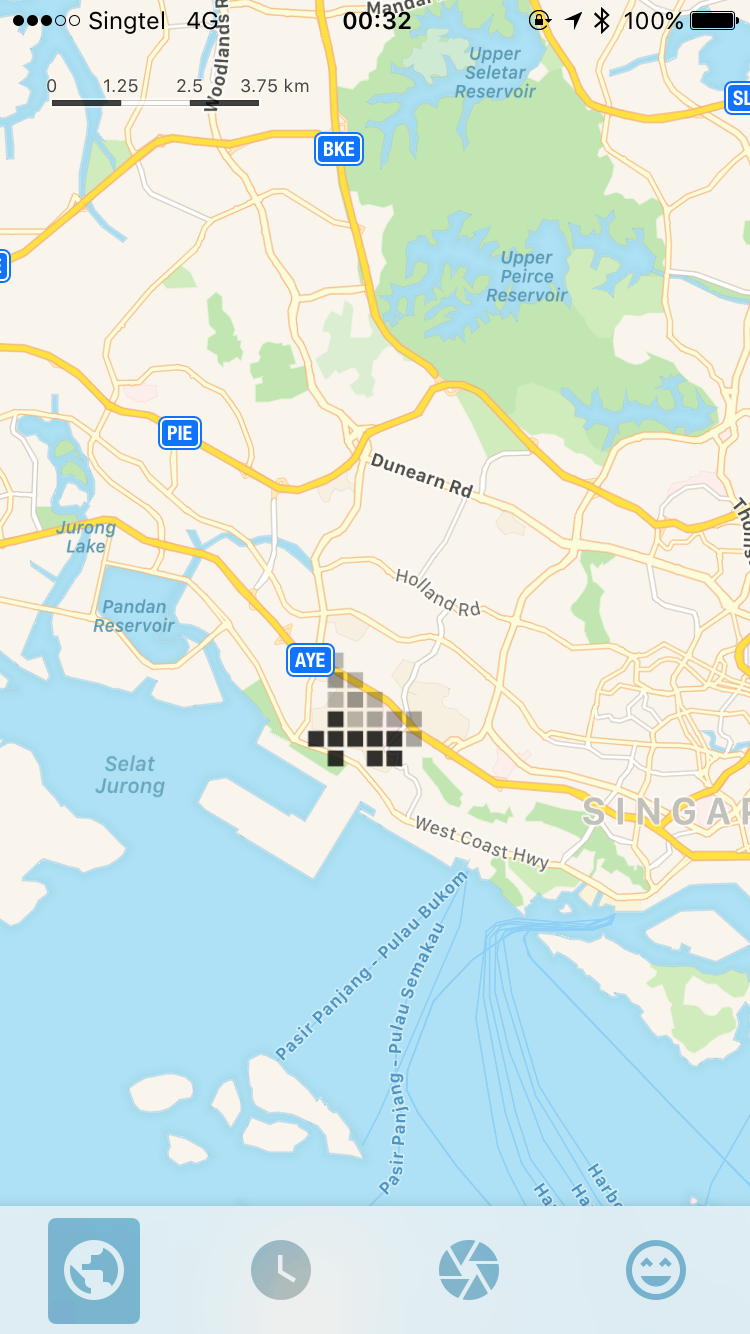
\includegraphics[width=0.32\textwidth]{4-1-4-a}
                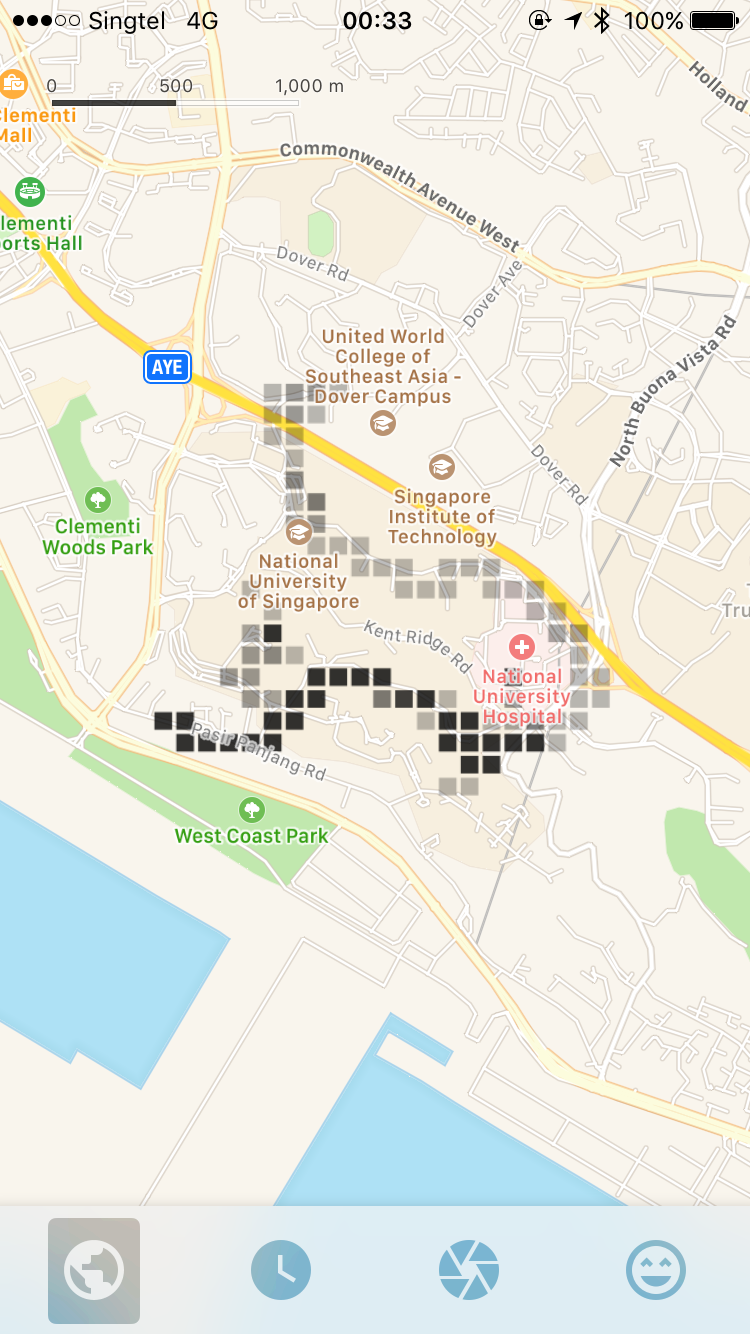
\includegraphics[width=0.32\textwidth]{4-1-4-c}
                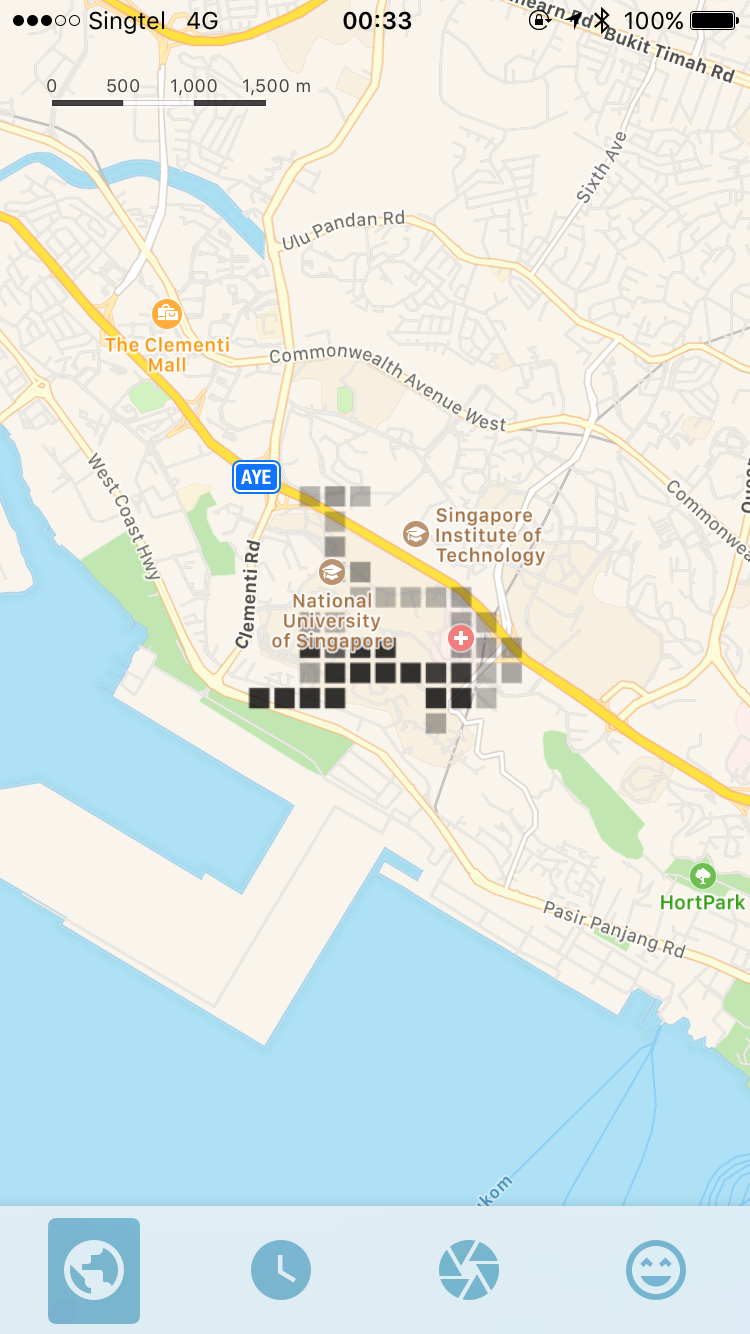
\includegraphics[width=0.32\textwidth]{4-1-4-b}
                \centering
                \caption{View aggregated records}
                \label{fig:aggregated-records}
            \end{figure}
            
            Aggregated records refer to all the places the user have been to. To visualize them on the map:
            \begin{enumerate}
                \item Select the first tab
                \item Scroll, zoom in or out to find the location of your interests
            \end{enumerate}
            As shown in Figure \ref{fig:aggregated-records}, the detail level will change as the user zooms in and out.
            
            \footnotesize
            Section \ref{sec:view-aggregated-records} is written by Jinghan.
            \normalsize
            
        \subsection{Record a New Path}
            \label{sec:record-new-path}
            \begin{figure}[H]
                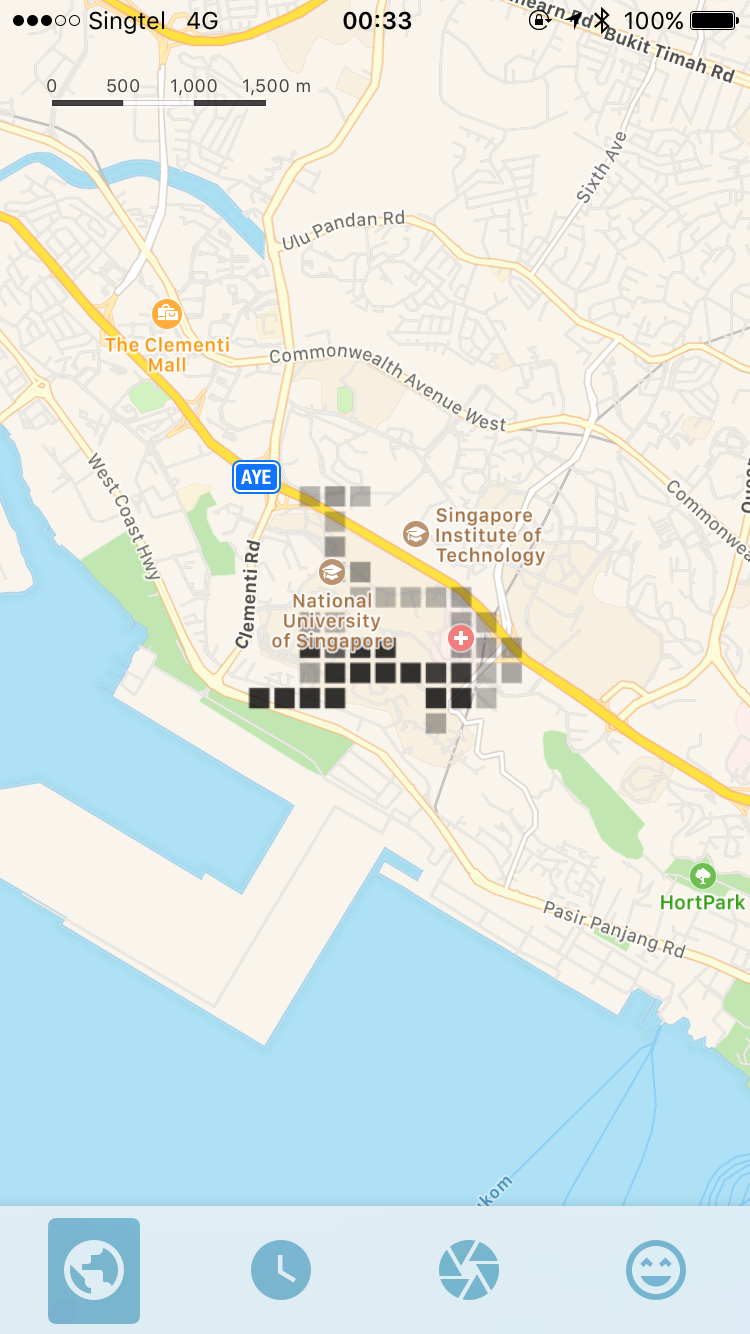
\includegraphics[width=0.32\textwidth]{4-1-4-b}
                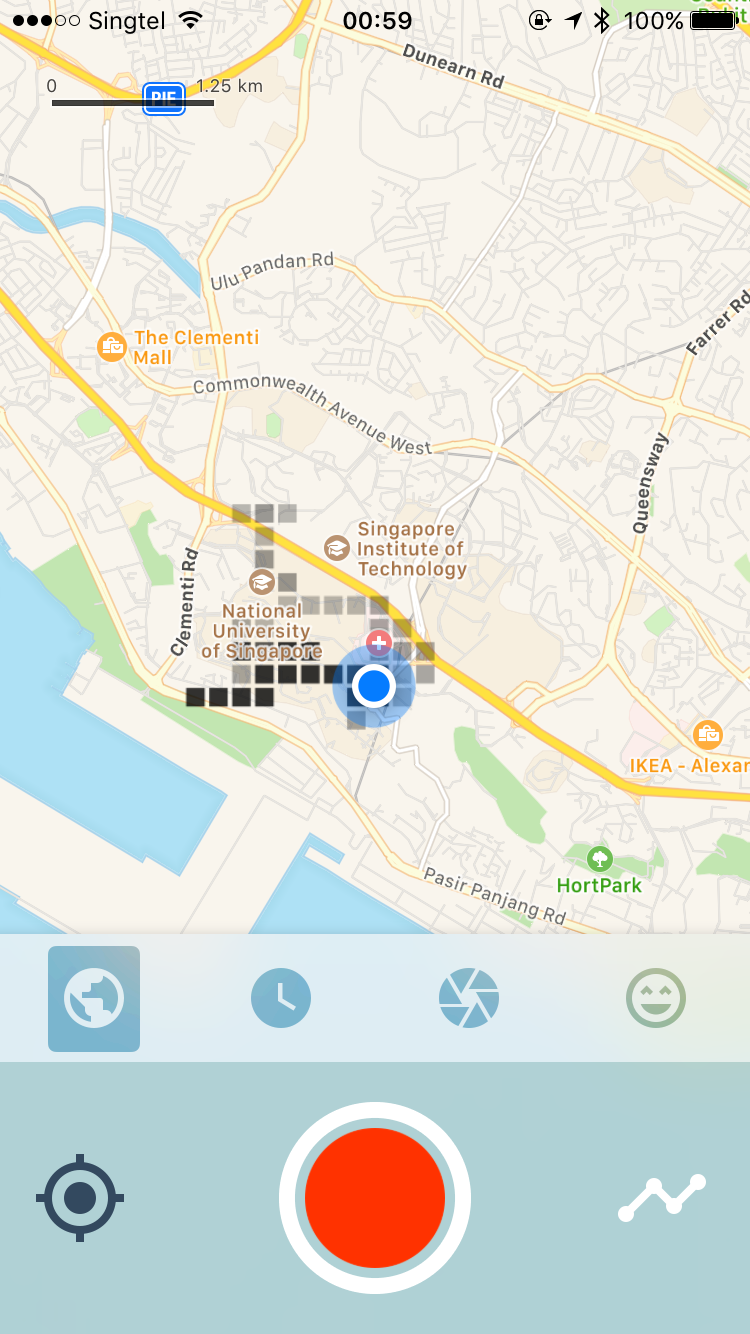
\includegraphics[width=0.32\textwidth]{2-2-a}
                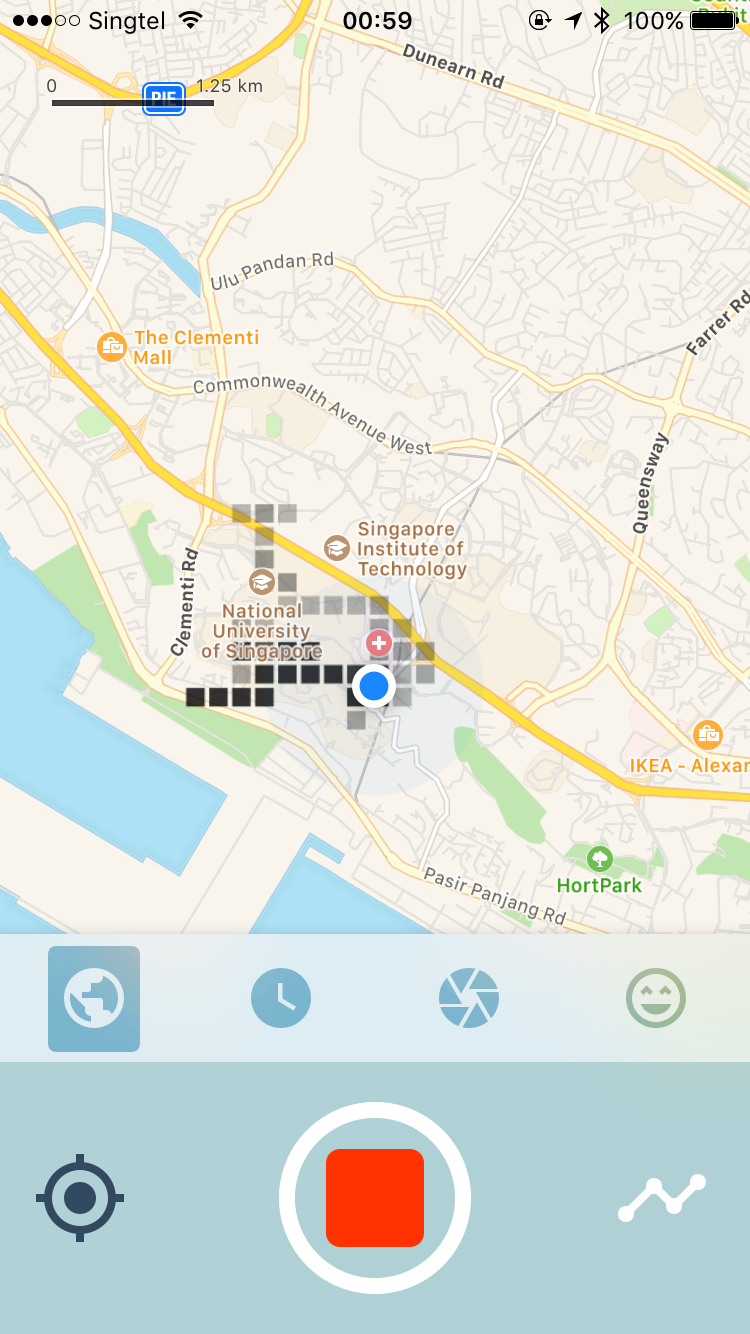
\includegraphics[width=0.32\textwidth]{2-2-b}
                \centering
                \caption{Record a new path}
                \label{fig:record-new-path}
            \end{figure}
            
            To record a new path, the user will need to:
            \begin{enumerate}
                \item Select the first tab
                \item Drag the tab bar out and snap it at the first level
                \item Tap on the round button in red
            \end{enumerate}
            As shown in Figure \ref{fig:aggregated-records}, the round button will transform to a square. The square record button indicates the application is now in the recording state. The user location button on the left is in dark blue. This means the application is in user tracking mode, in which the region that the map view shows will be updated so that the user location marker is always at the center of the screen.
            
            \footnotesize
            Section \ref{sec:record-new-path} is written by Jinghan.
            \normalsize
        
        
        \subsection{View All Recorded Paths} % Wang
            \label{sec:view-all-recorded-paths}
            \subsubsection{View the path lists}
            \label{sec:view-path-list}
            \begin{figure}[H]
                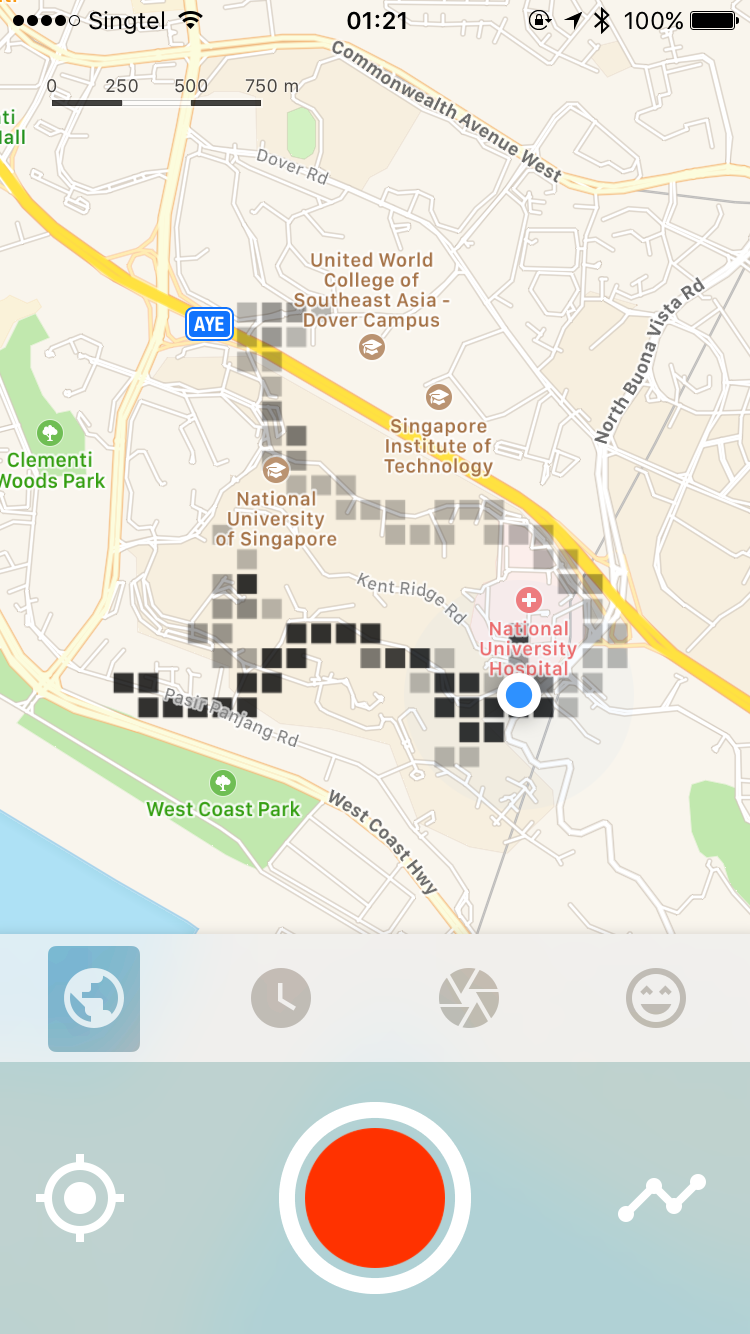
\includegraphics[width=0.32\textwidth]{2-3-1-a}
                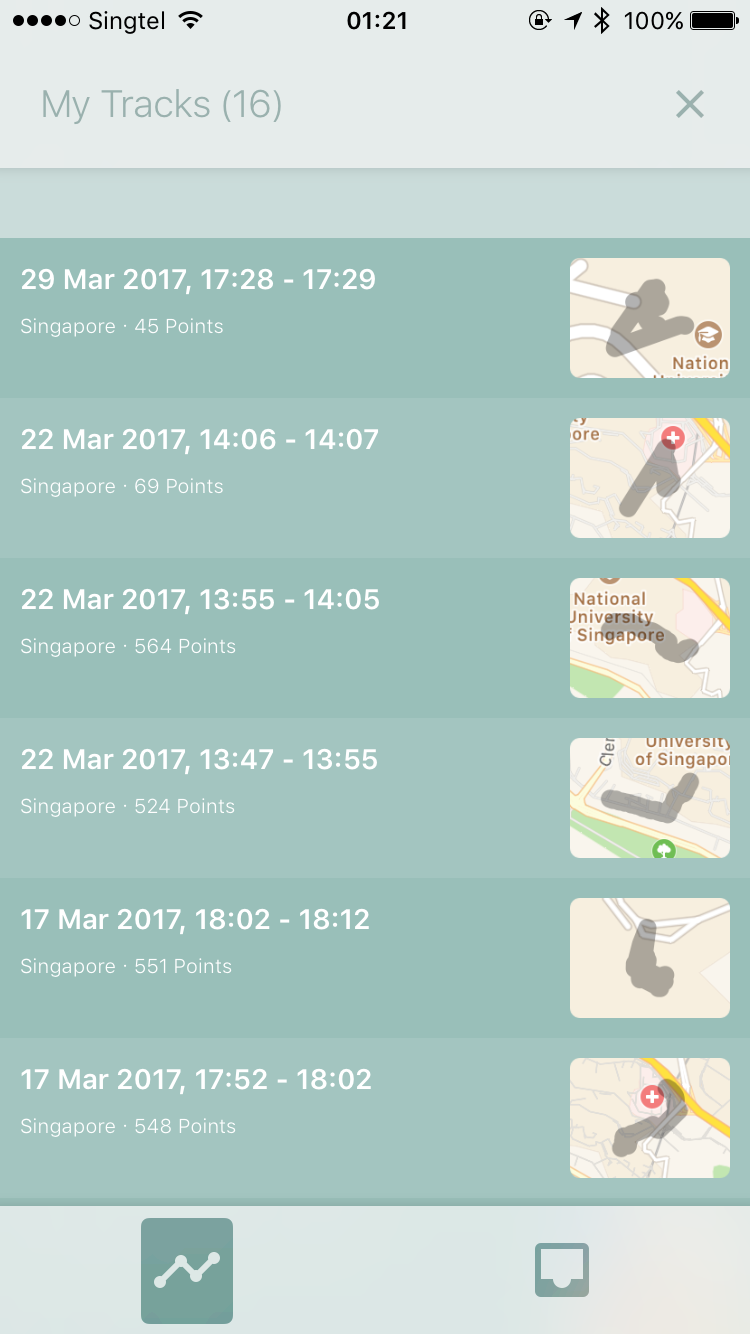
\includegraphics[width=0.32\textwidth]{2-3-1-b}
                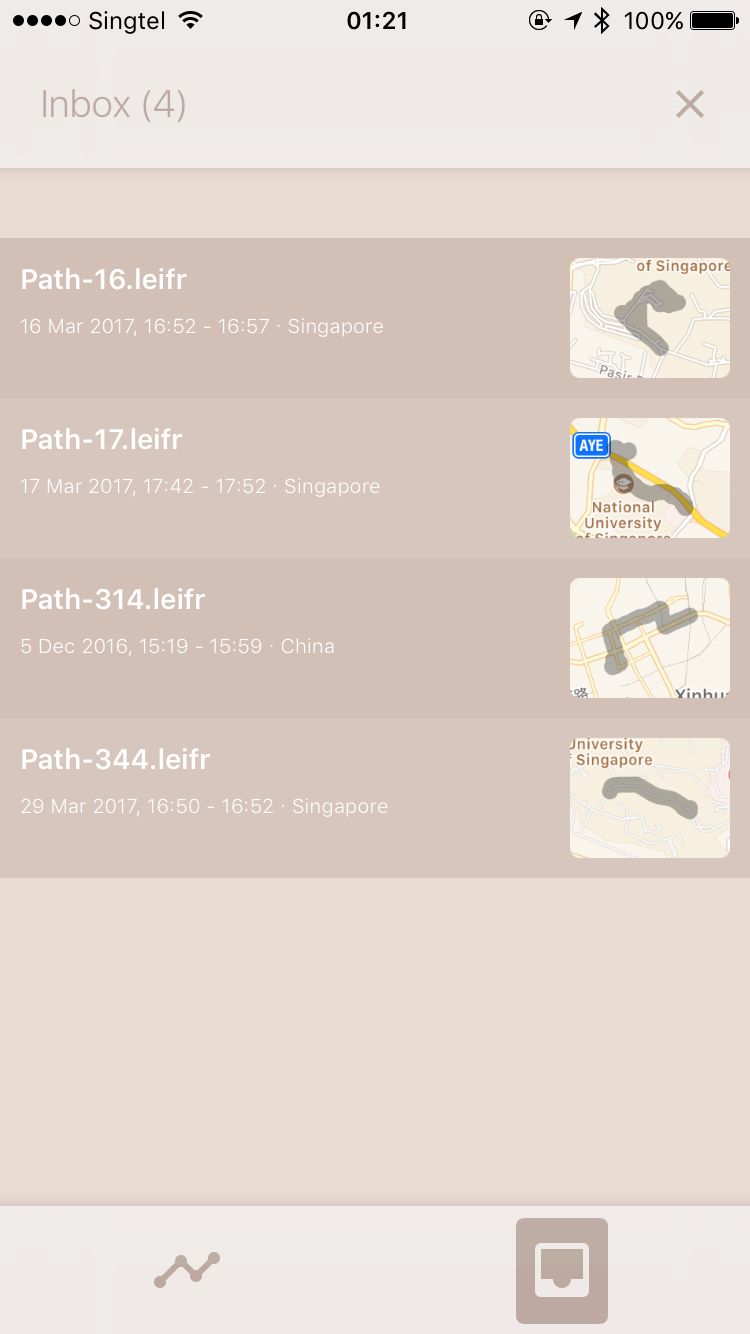
\includegraphics[width=0.32\textwidth]{2-3-1-c}
                \centering
                \caption{View the path lists}
                \label{fig:view-path-list}
            \end{figure}
            
            To view the lists of all available paths, the user will need to:
            \begin{enumerate}
                \item Select the first tab
                \item Drag the tab bar out and snap it at the first level
                \item Tap on path icon on the right hand side of the control panel
                \item Select either the ``My Track'' tab or the ``Inbox'' tab
                \item Tap the ``Load More'' button if more paths are desired
            \end{enumerate}
            As shown in Figure \ref{fig:view-path-list}, a new view will be presented after tapping on the path icon. In the presented view, the user's own paths will be shown with a green background while the paths he or she received from his or her friends will be shown in a red background.
            
            \subsubsection{Share or delete a path}
            
            \begin{figure}[H]
                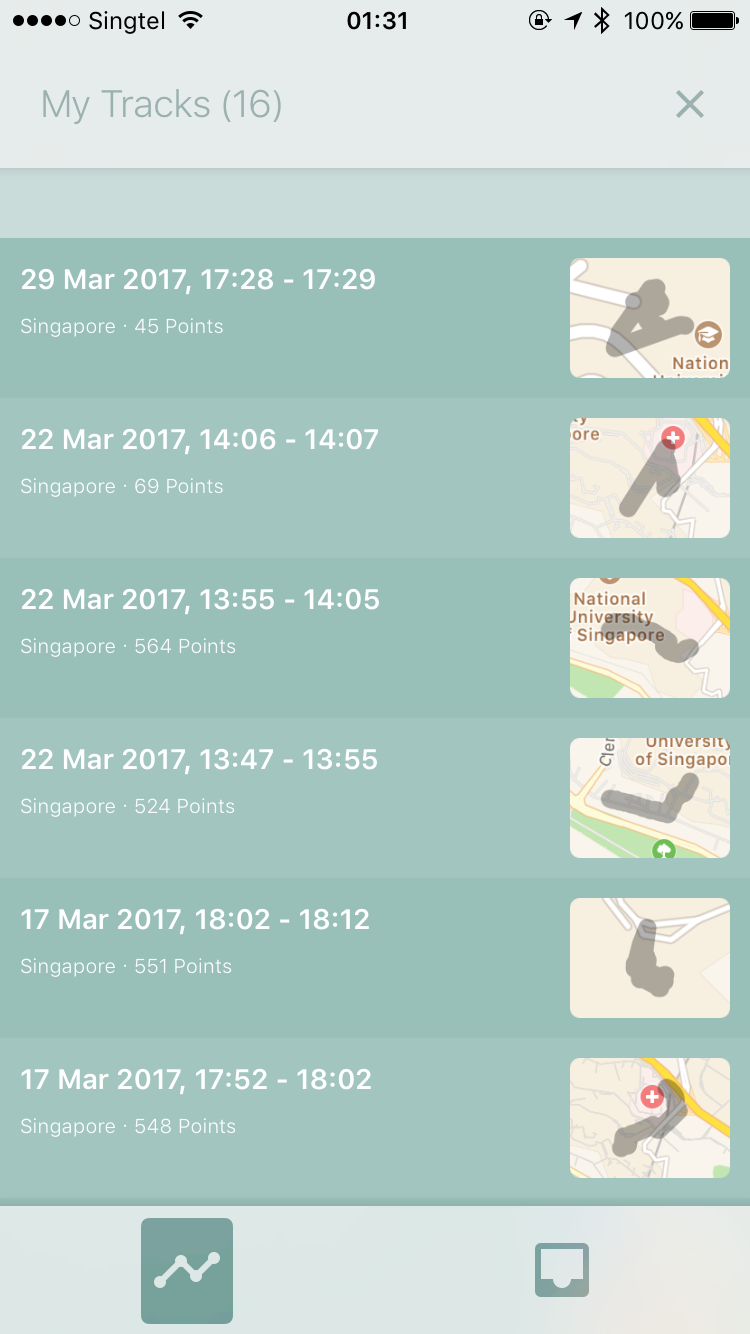
\includegraphics[width=0.32\textwidth]{2-3-2-a}
                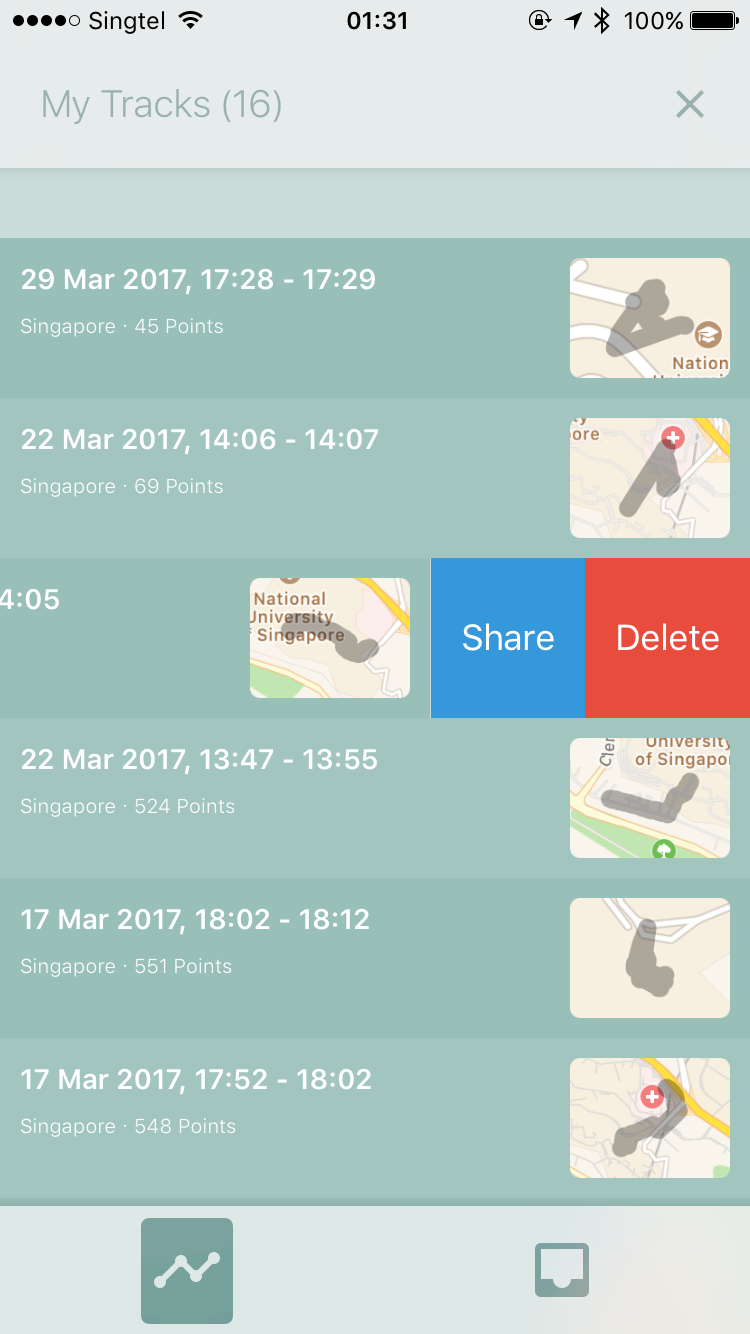
\includegraphics[width=0.32\textwidth]{2-3-2-b}
                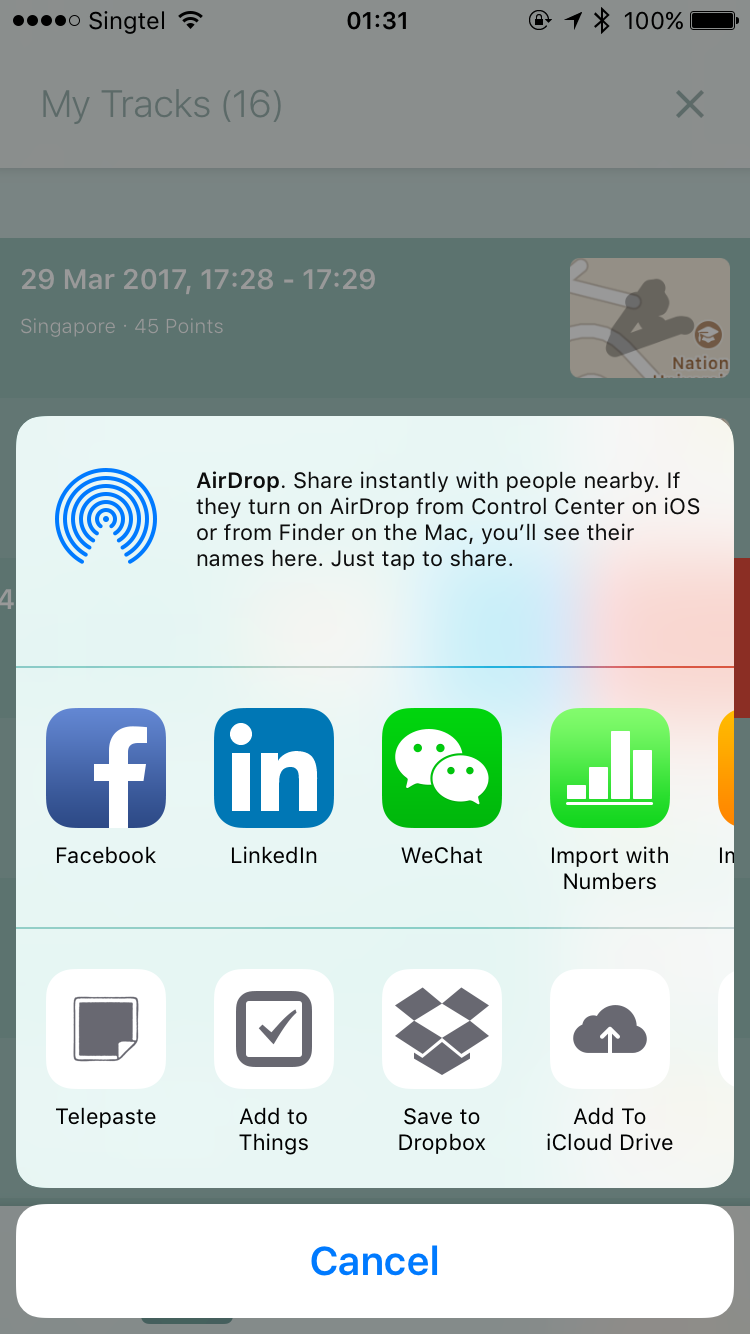
\includegraphics[width=0.32\textwidth]{2-3-2-c}
                \centering
                \caption{Share or delete a path}
                \label{fig:share-delete-path}
            \end{figure}
            
            To share a path, the user will need to:
            \begin{enumerate}
                \item Go to the path list view as in section \ref{sec:view-path-list}
                \item Drag the cell which contains the target path to the left
                \item Tap the blue ``Share'' button
                \item Select the application to send the path
            \end{enumerate}
            
            After the application is selected, an file with an extension of \texttt{.leifr} will be delegated to that particular application.
            
            To delete a path, the user will need to:
            \begin{enumerate}
                \item Repeat the first two steps as in ``To share a path''
                \item Tap the red ``Delete'' button. Please note that this action cannot be recovered
            \end{enumerate}
            
            \footnotesize
            Section \ref{sec:view-all-recorded-paths} is written by Jinghan.
            \normalsize
            
        \subsection{Replay Paths} % Lei
            \label{sec:replay-paths}
            Playing back a path animation can be divided into two sub-tasks: path selection and path playback control, where the former sub-task is the pre-condition of the latter one.
            
            \subsubsection{Select Paths}
                \label{sec:select-path}
                In the application, two different ways are provided to complete the path(s) selection: one is from the path lists in the history overview page and the other is from the calendar in path playback page.
                \paragraph{Select a Path From Path Lists}
                \begin{figure}[H]
                    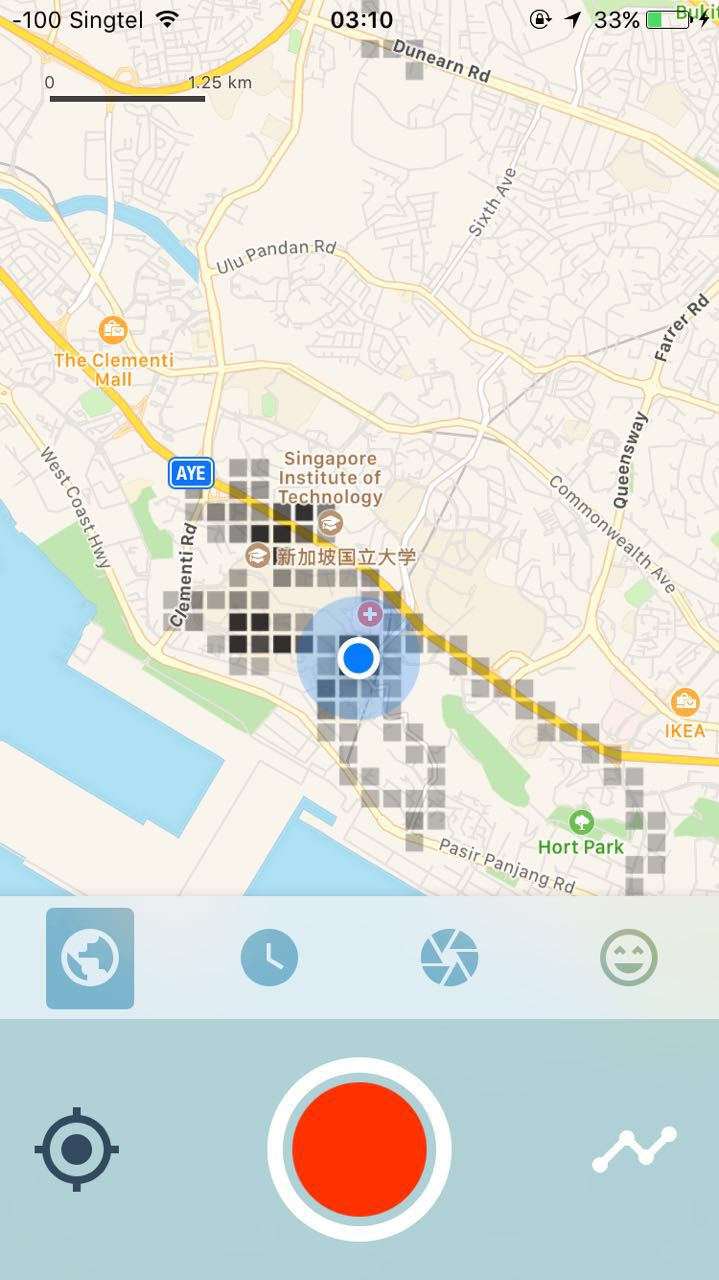
\includegraphics[width=0.32\textwidth]{2-4-1-1-a}
                    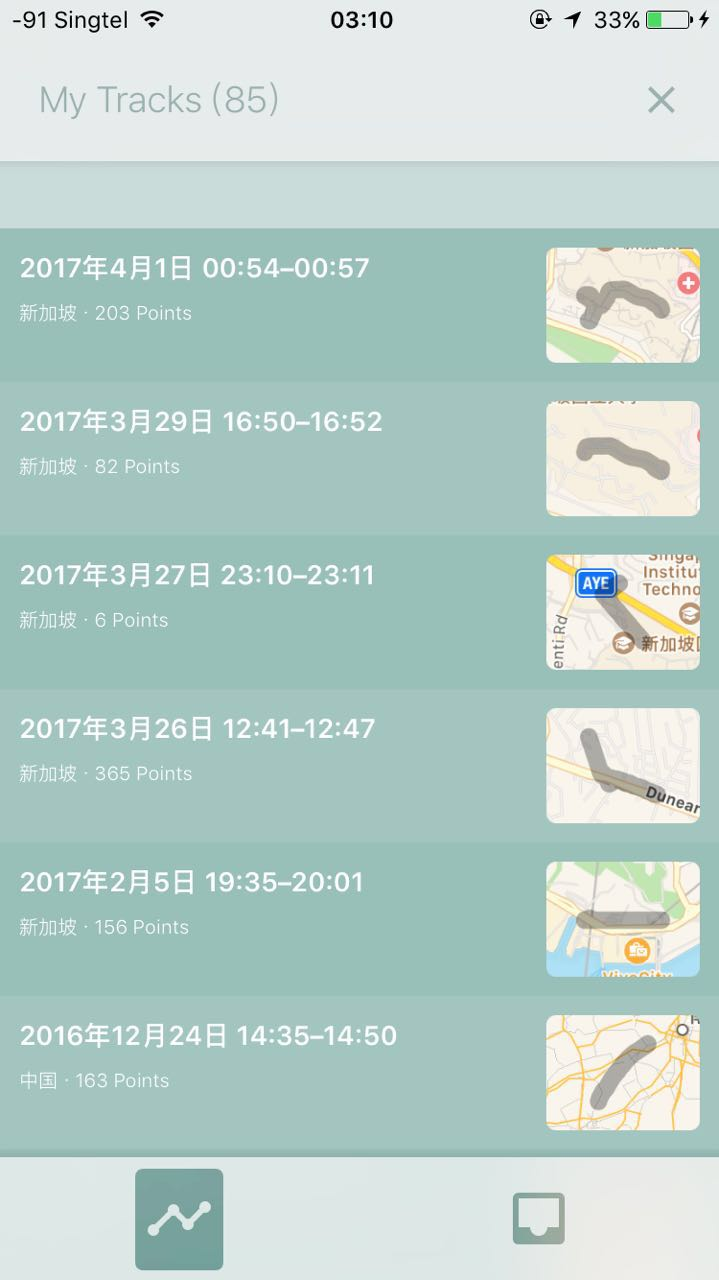
\includegraphics[width=0.32\textwidth]{2-4-1-1-b}
                    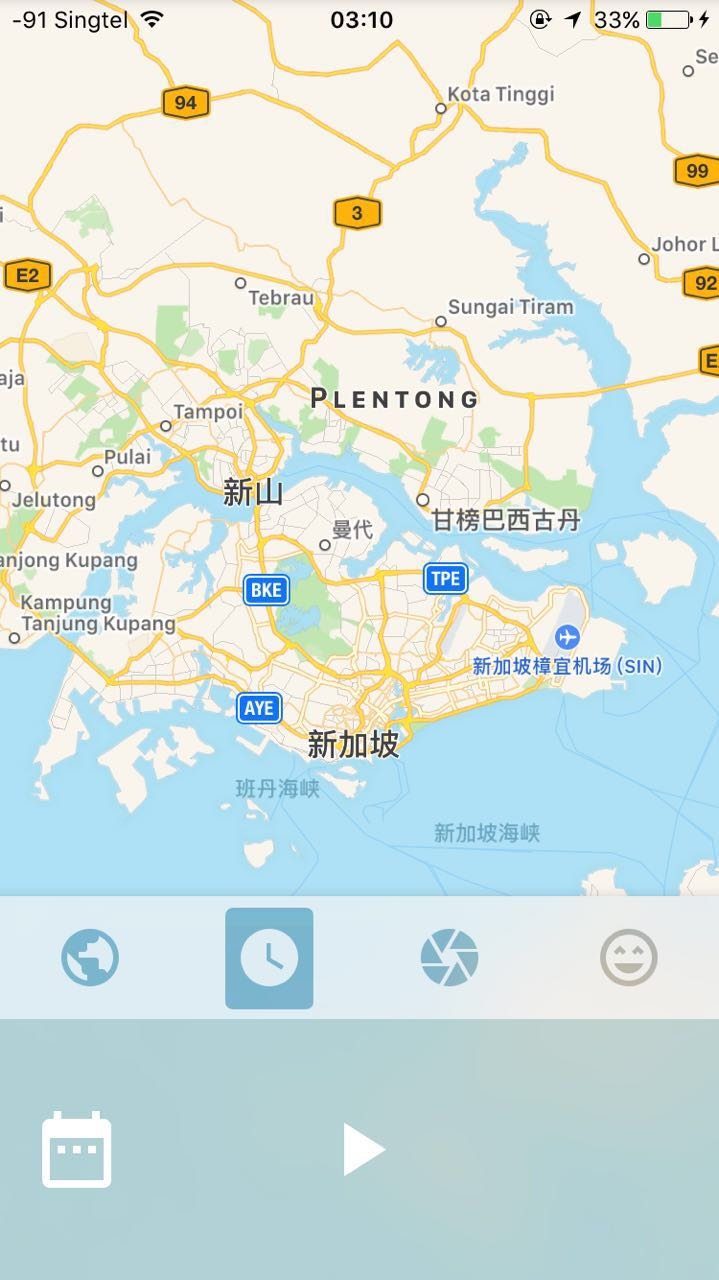
\includegraphics[width=0.32\textwidth]{2-4-1-1-c}
                    \centering
                    \caption{Select a path from the path lists}
                    \label{fig:select-path-lists}
                \end{figure}
                
                To select a path from the path lists, the user will need to:
                \begin{enumerate}
                    \item Go to the path list view as in Section \ref{sec:view-path-list}.
                    \item Switch to the correct page depending on whether the user wants to select a path from the recorded paths list or the received paths list.
                    \item Tap on the path to be played back.
                \end{enumerate}
                
                After the path is selected, the user will be directed to the path playback view, where he or she can control the path playing as describe in Section \ref{sec:playback-control}.
                
                \paragraph{Select Paths Starting From Some Date}
                \begin{figure}[H]
                    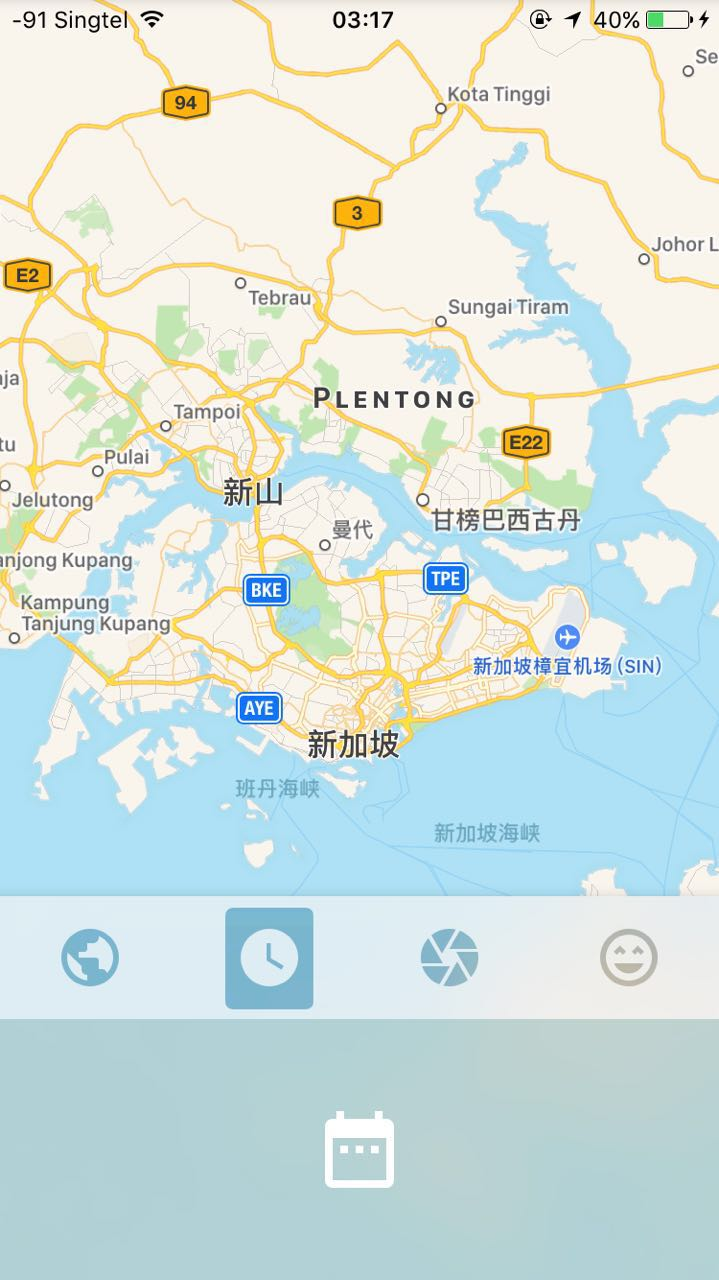
\includegraphics[width=0.32\textwidth]{2-4-1-2-a}
                    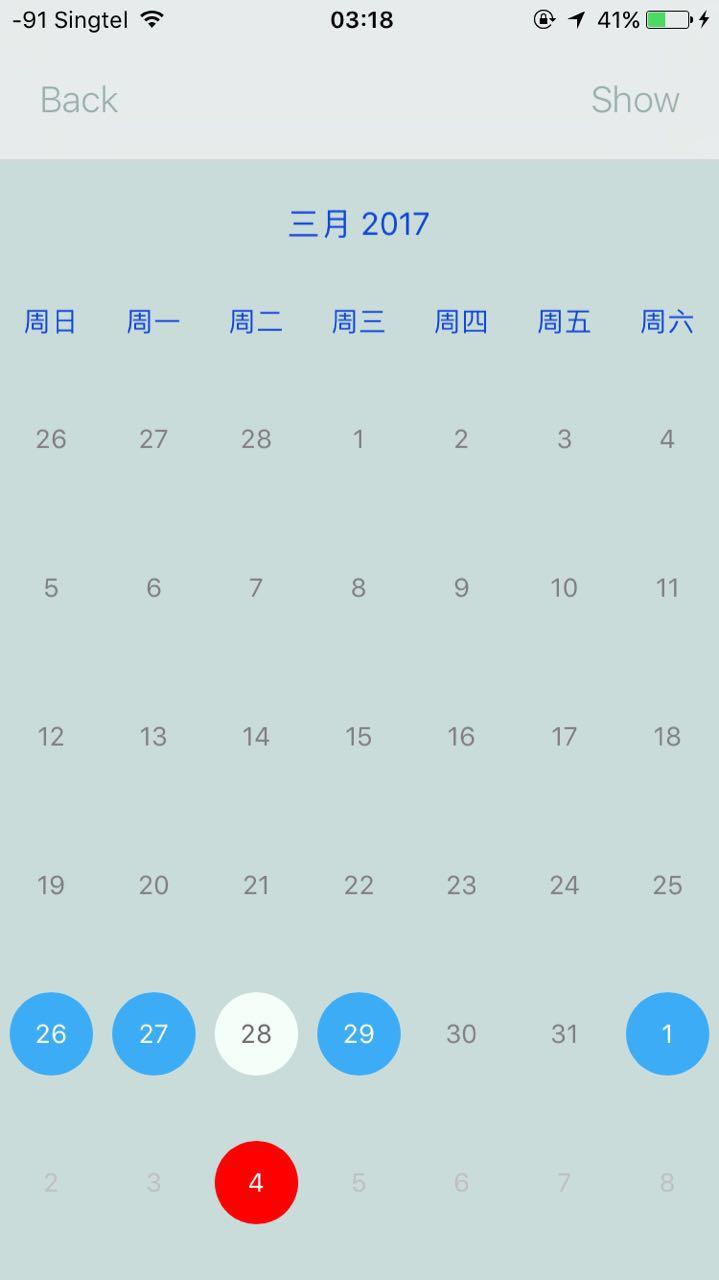
\includegraphics[width=0.32\textwidth]{2-4-1-2-b}
                    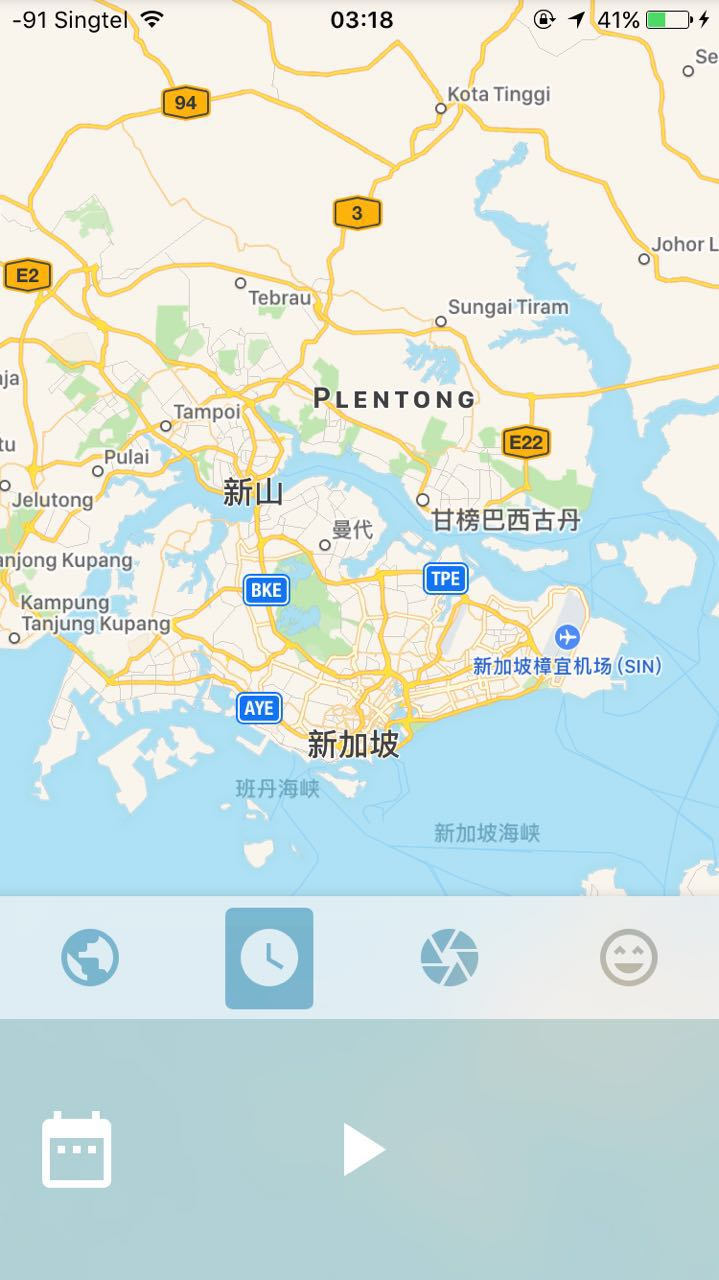
\includegraphics[width=0.32\textwidth]{2-4-1-2-c}
                    \centering
                    \caption{Select a path from the calendar picker}
                    \label{fig:select-path-calendar}
                \end{figure}
                
                To select a list of paths starting from some date, the user will need to:
                \begin{enumerate}
                    \item Select the second tab
                    \item Drag the tab bar out and snap it at the first level
                    \item Tap on the calendar button
                    \item Scroll to the correct month of the starting date
                    \item Select and highlight the starting date (the date with white background in Figure \ref{fig:select-path-calendar})
                    \item Tap on the ``Show'' button at the top-right corner
                \end{enumerate}
                
                After starting date is selected, the user will be directed back to the path playback view, where he or she can control the path playing as describe in Section \ref{sec:playback-control}.
                
            \subsubsection{Playback Control}
                \label{sec:playback-control}
                
                After the user successfully selects the path(s) as describe in Section \ref{sec:select-path}, the user can start to control the playback animation. In general, there are four different operations the user can perform, namely start, pause, resume and stop.
                
                \paragraph{Start the Animation}
                \label{sec:start-animation}
                \begin{figure}[H]
                    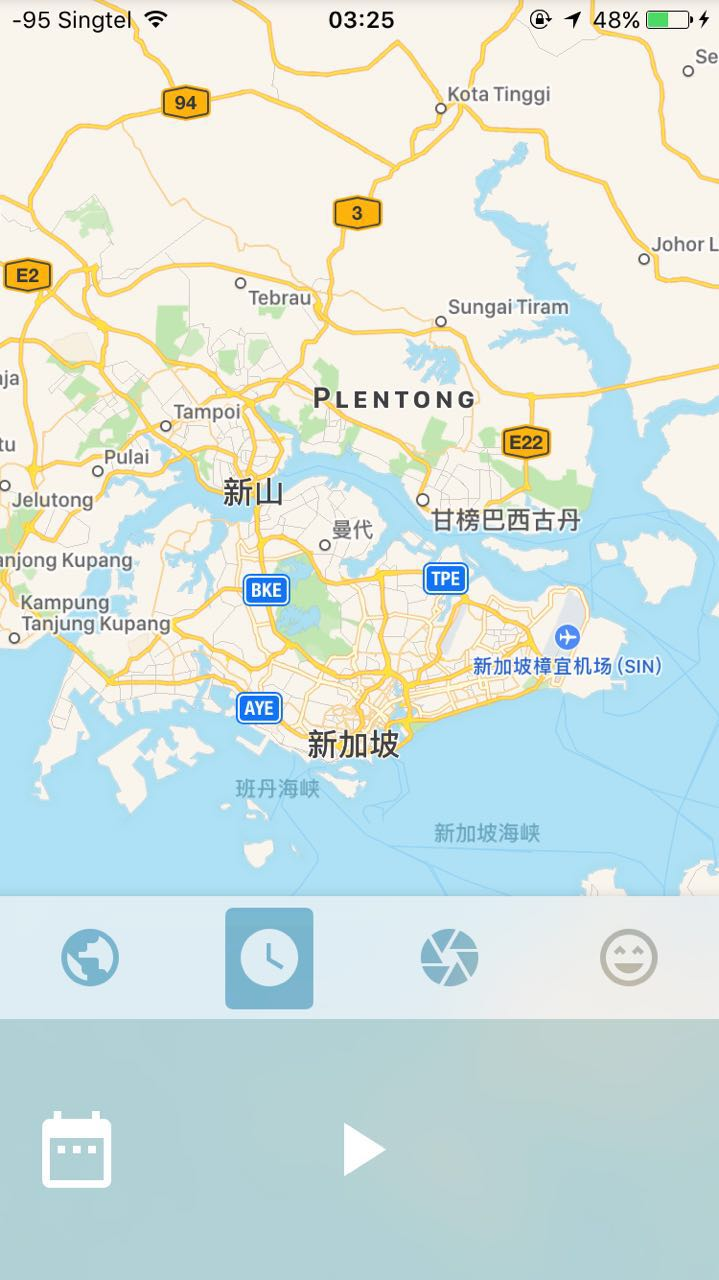
\includegraphics[width=0.32\textwidth]{2-4-2-1-a}
                    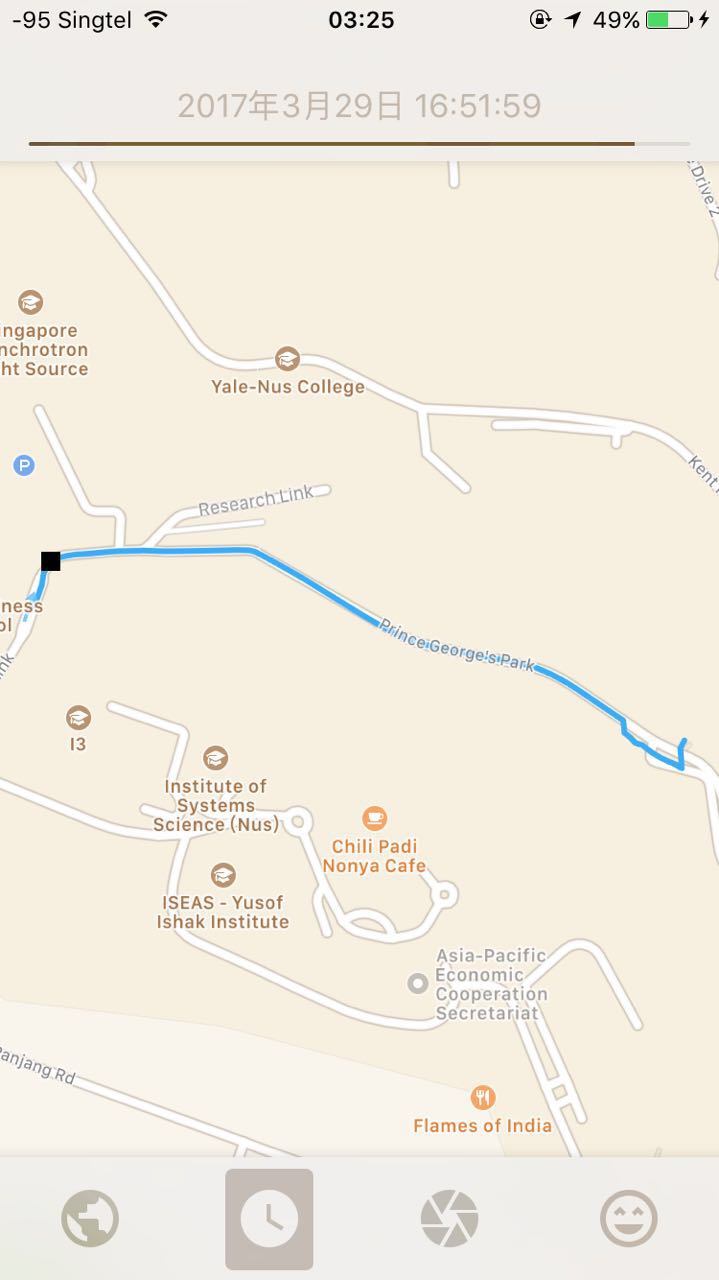
\includegraphics[width=0.32\textwidth]{2-4-2-1-b}
                    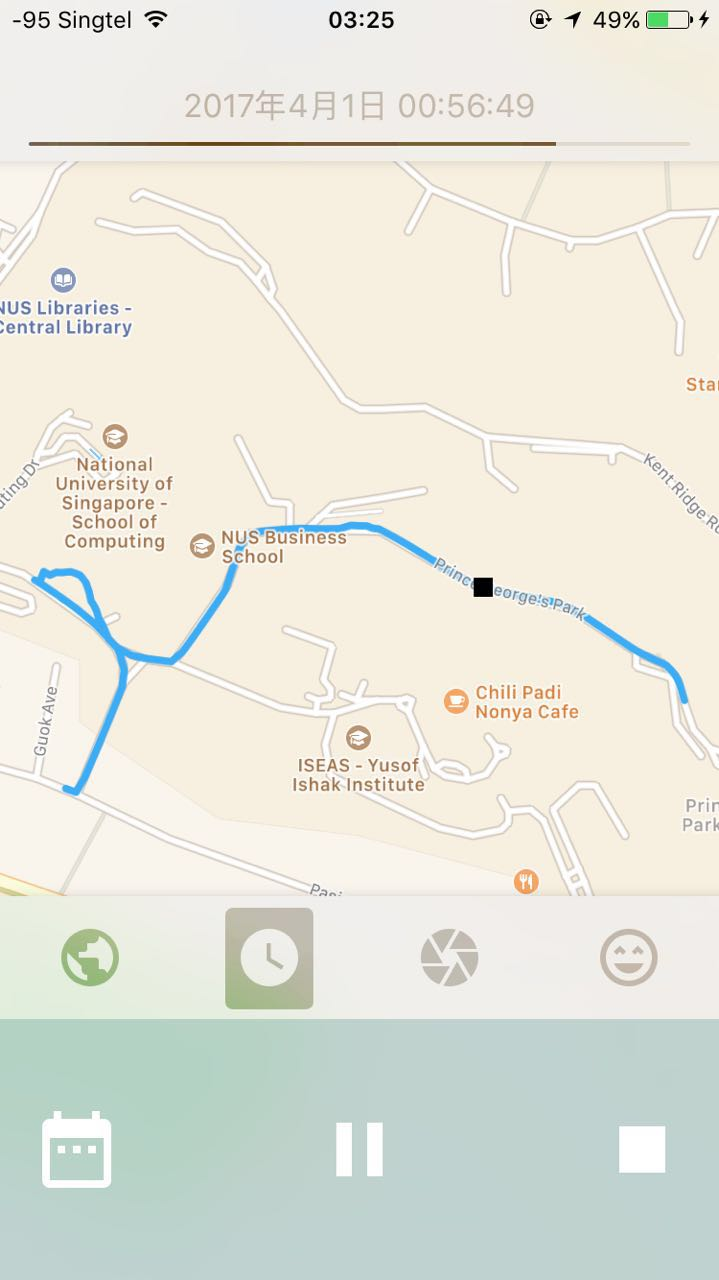
\includegraphics[width=0.32\textwidth]{2-4-2-1-c}
                    \centering
                    \caption{Start the animation}
                    \label{fig:start-animation}
                \end{figure}
                
                To start the playback animation, the user will need to:
                \begin{enumerate}
                    \item Select the path(s) as describe in Section \ref{sec:select-path}.
                    \item Tap on the play button
                \end{enumerate}
                
                After the animation starts to play, the hover tab will be collapsed and a new header view showing the time information for the current annotation point will appear (see Figure \ref{fig:start-animation}, middle). If the user select multiple paths from the calendar, after the animation of one path finished, the system will pause for 0.5 second before continuing to play the next path (see Figure \ref{fig:start-animation}, right). If all the paths have been played, the animation will be stopped.
                
                \paragraph{Pause and Resume the Animation}
                \begin{figure}[H]
                    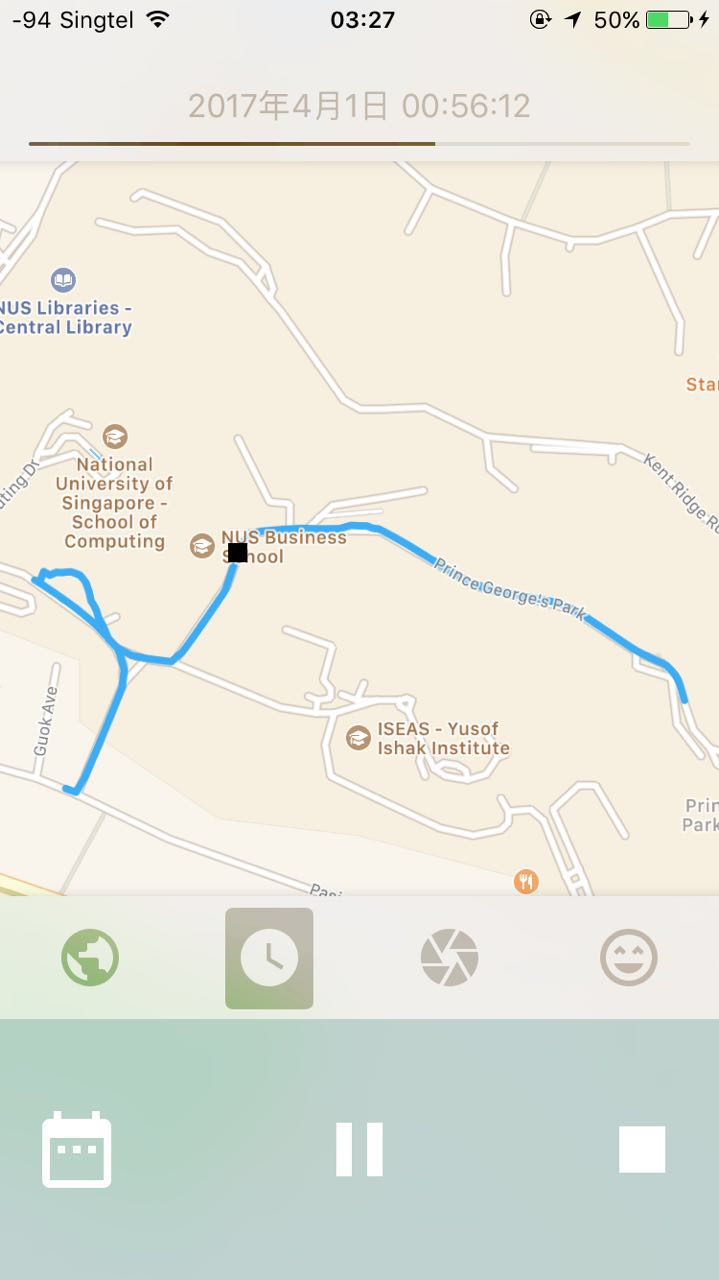
\includegraphics[width=0.32\textwidth]{2-4-2-2-a}
                    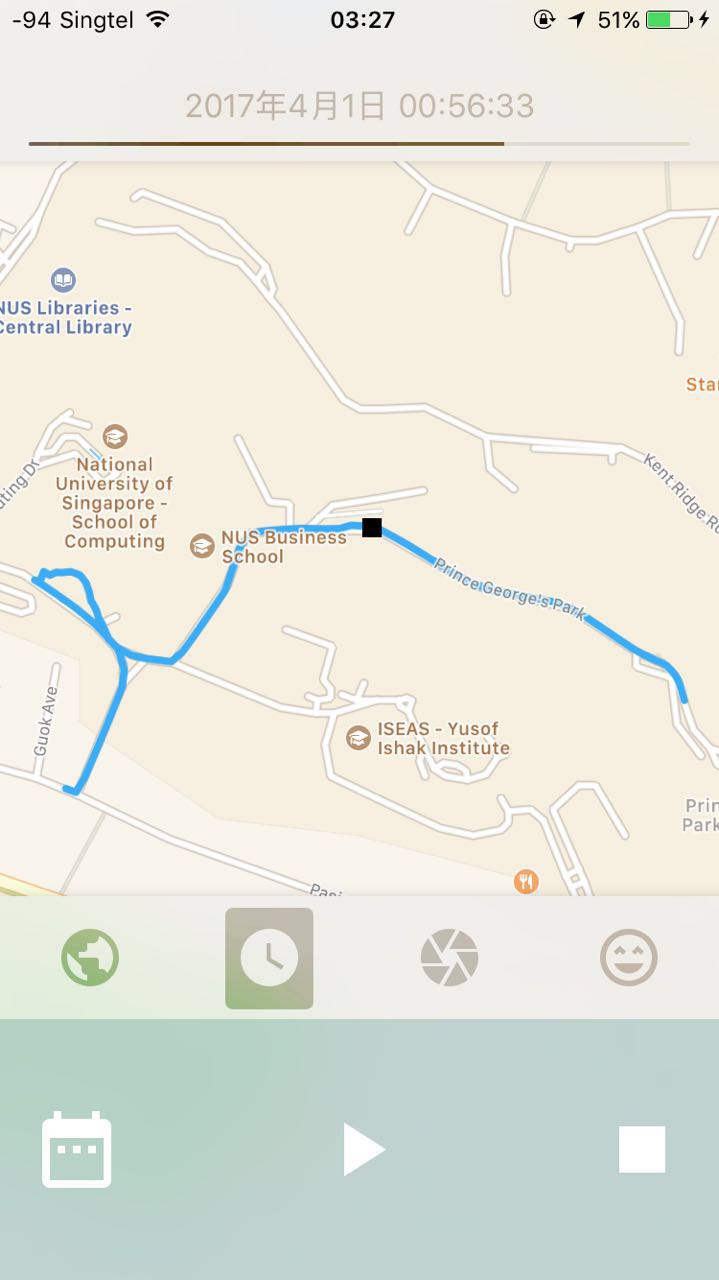
\includegraphics[width=0.32\textwidth]{2-4-2-2-b}
                    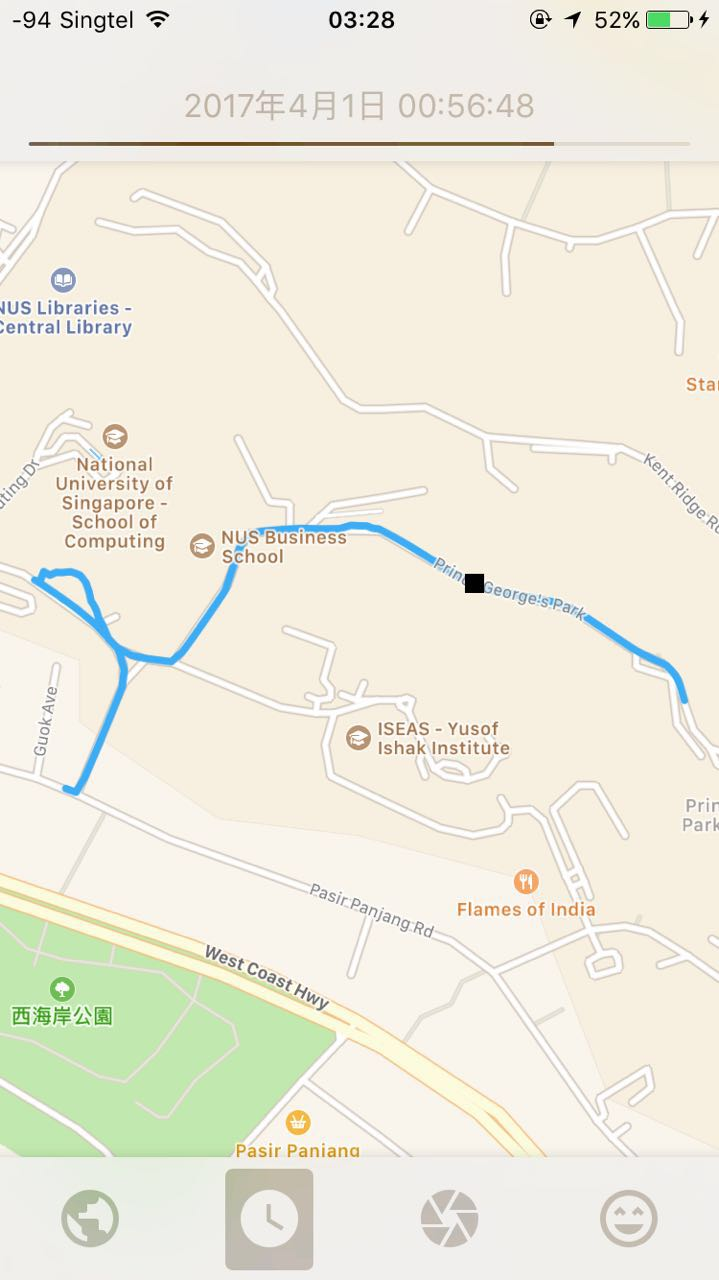
\includegraphics[width=0.32\textwidth]{2-4-2-2-c}
                    \centering
                    \caption{Pause and resume the animation}
                    \label{fig:pause-resume-animation}
                \end{figure}
                
                To pause the playback animation, the user will need to:
                \begin{enumerate}
                    \item Drag the tab bar out and snap it at the first level, since the tab bar will be collapse once the user starts the animation. The result of this step is shown in Figure \ref{fig:pause-resume-animation}, left.
                    \item Tap on the pause button.
                \end{enumerate}
                
                To resume the playback animation, the user will need to:
                \begin{enumerate}
                    \item Tap on the resume button, which is the same as the play button.
                \end{enumerate}
                
                The user has the freedom to pause and resume the path animation by any number of times before the animation ends. The user can also drag the map or zoom in/out while the animation is being played.
                
                \paragraph{Stop the Animation}
                \begin{figure}[H]
                    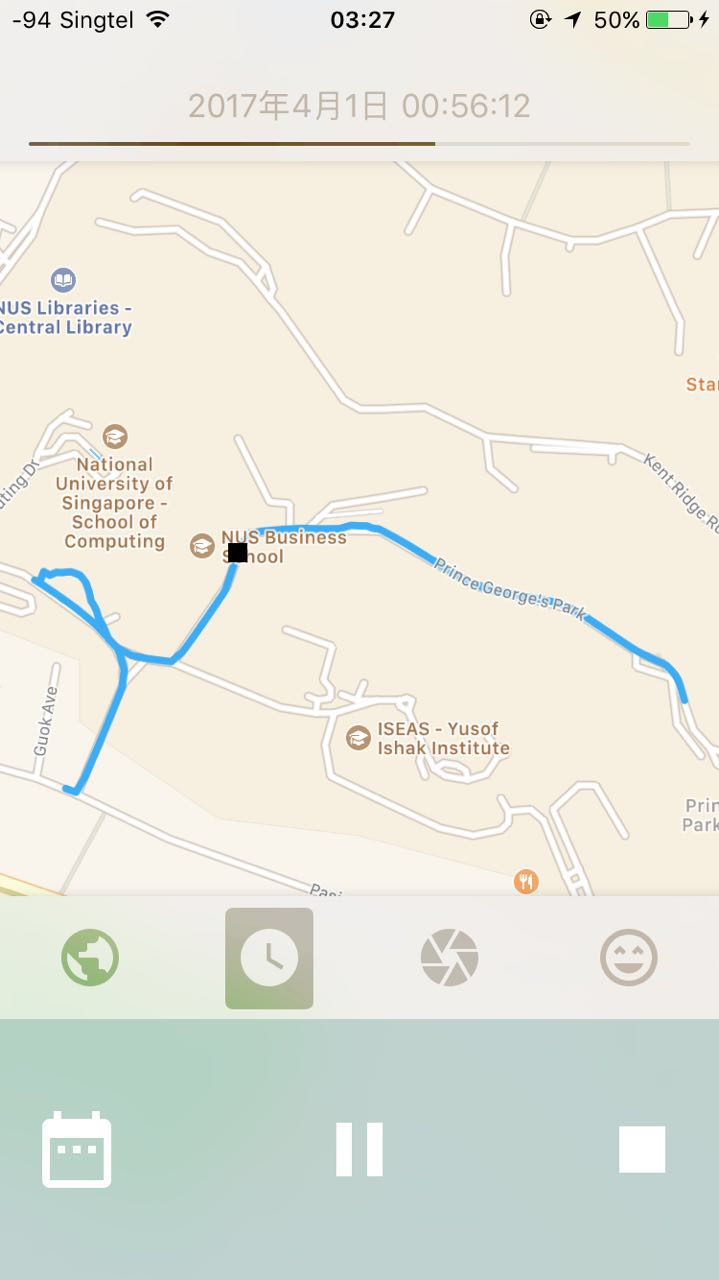
\includegraphics[width=0.32\textwidth]{2-4-2-3-a}
                    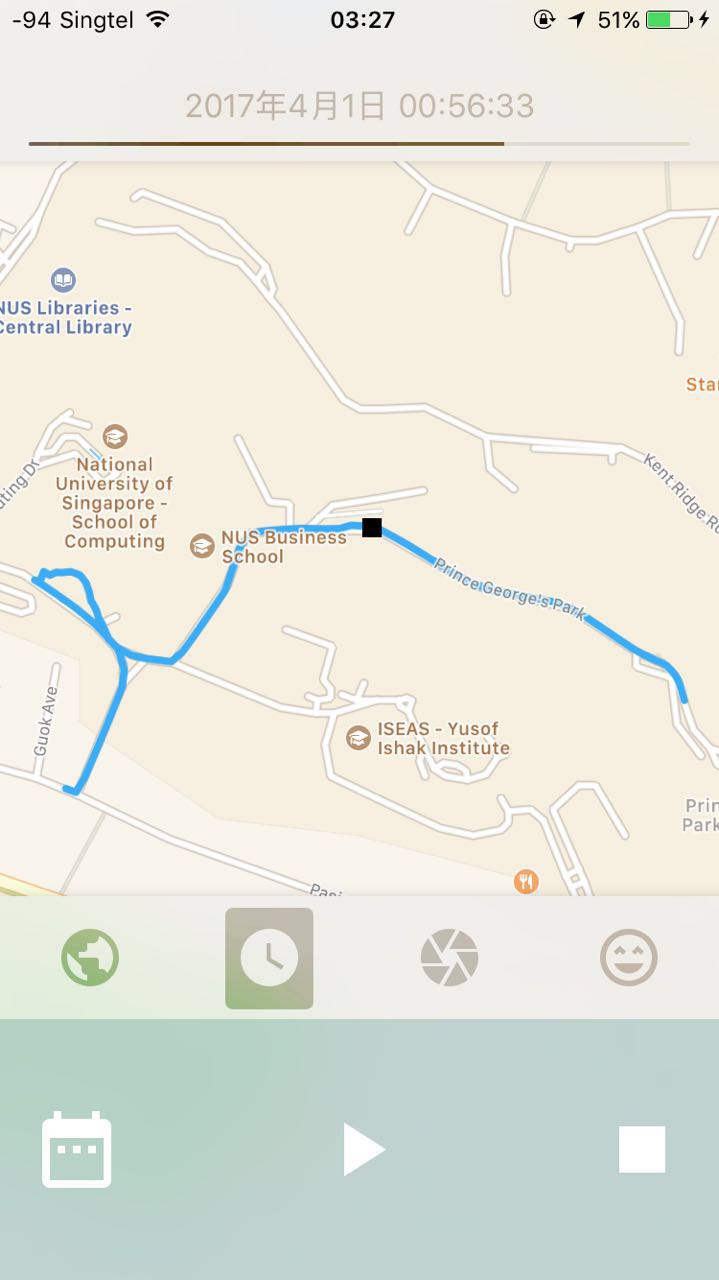
\includegraphics[width=0.32\textwidth]{2-4-2-3-b}
                    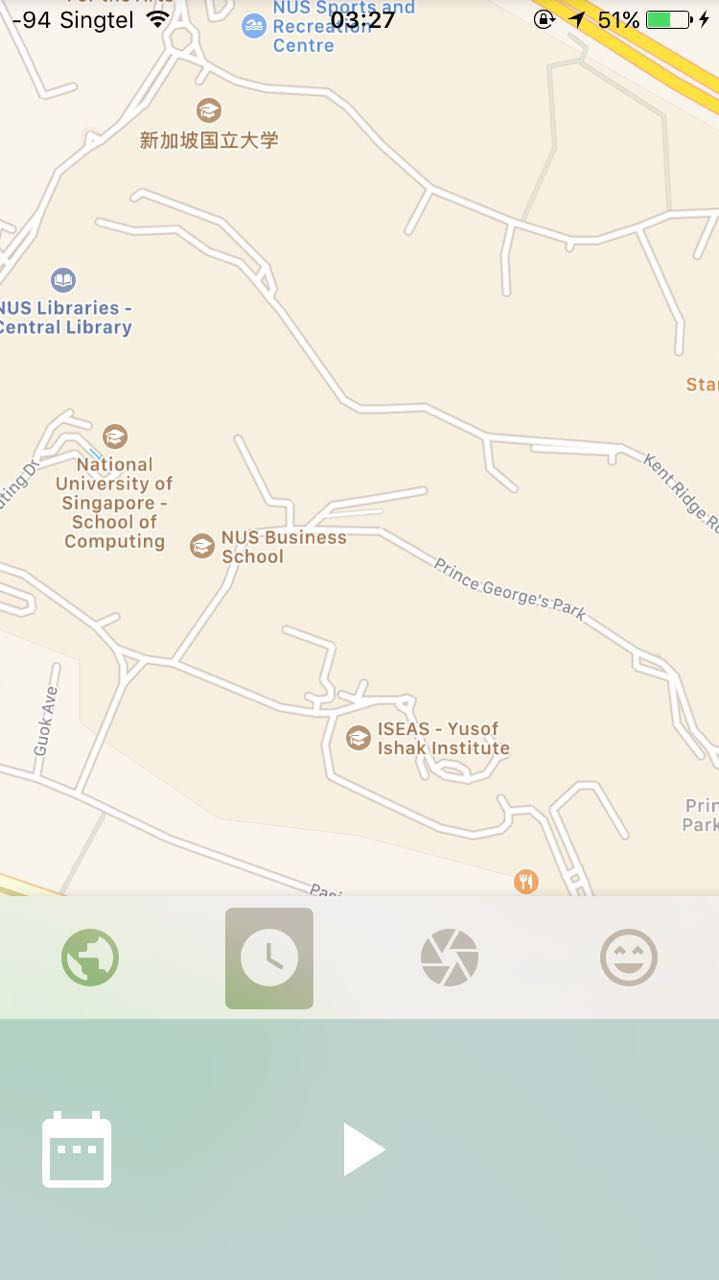
\includegraphics[width=0.32\textwidth]{2-4-2-3-c}
                    \centering
                    \caption{Stop the animation}
                    \label{fig:stop-animation}
                \end{figure}
                
                To stop the playback animation, the user will need to:
                \begin{enumerate}
                    \item Drag the tab bar out and snap it at the first level, since the tab bar will be collapse once the user starts the animation. The result of this step is shown in Figure \ref{fig:stop-animation}, left.
                    \item Tap on the stop button.
                \end{enumerate}
                
                After the user stops the animation, the path together with the annotation marker will be removed from the map, the header view showing the time information will also disappear. The user can tap on the start button again to start the animation from the beginning just like in Section \ref{sec:start-animation}.
            
            \footnotesize
            Section \ref{sec:replay-paths} is written by Mingyu.
            \normalsize
        \clearpage
        
        \subsection{Locate a Photo} % Wang
            \label{sec:locate-photo}
            \begin{figure}[H]
                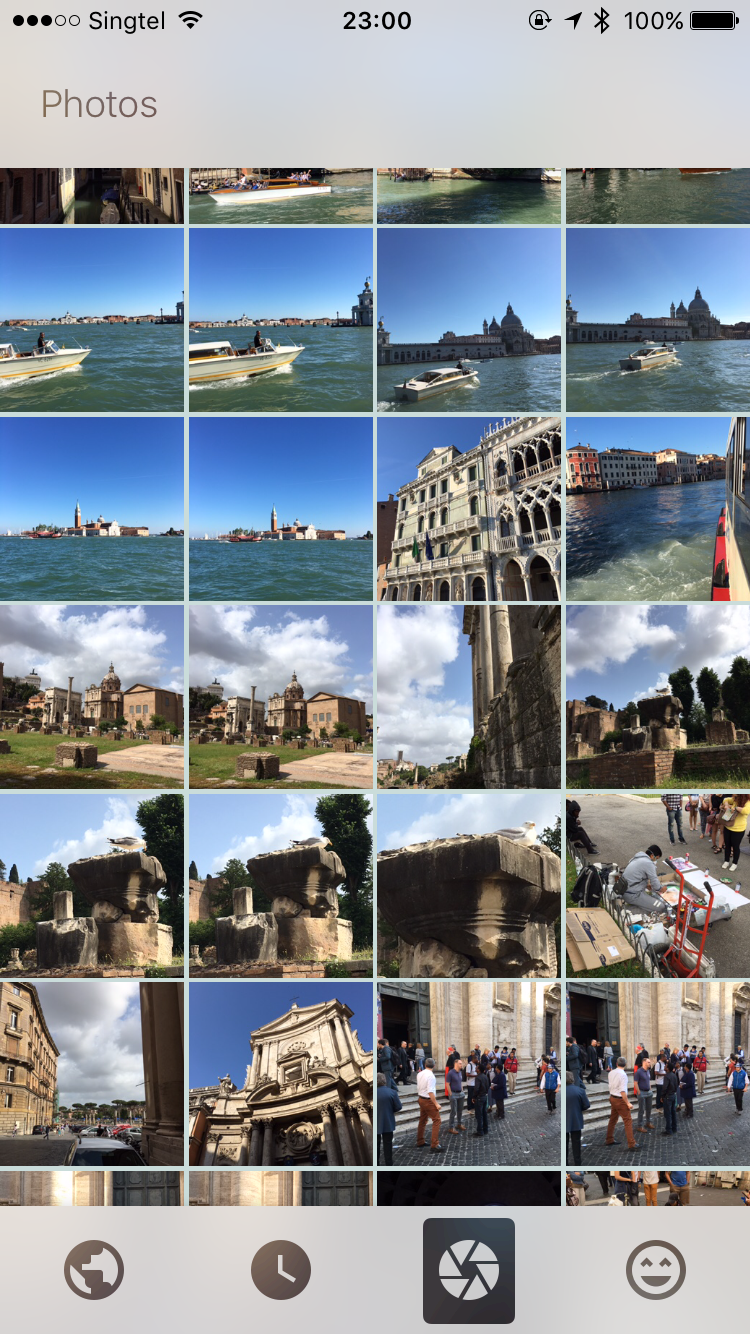
\includegraphics[width=0.32\textwidth]{4-1-6-a}
                
\includegraphics[width=0.32\textwidth]{4-1-6-b}
                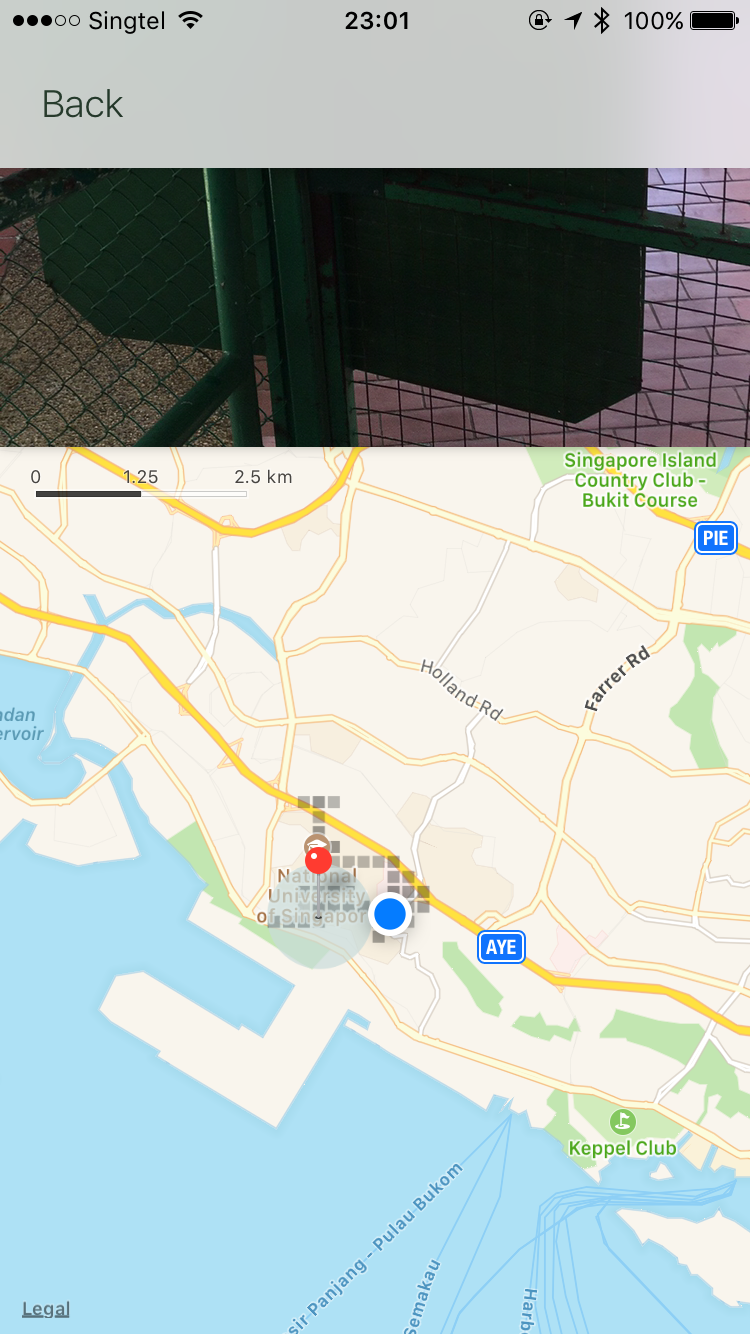
\includegraphics[width=0.32\textwidth]{4-1-6-c}
                \centering
                \caption{Locate a photo}
                \label{fig:locate-photo}
            \end{figure}
            
            To check the location/estimation of a photo, the user will need to:
            \begin{enumerate}
                \item Select the third tab
                \item Browse through the photo list
                \item Tap on the photo he or she is interested in
                \item Drag the photo up in the new view presented
                \item Zoom in or out as he or she likes
            \end{enumerate}
            As shown in Figure \ref{fig:locate-photo}, if the location of the selected photo is an estimation according the geo-location data stored in the database, the error will be shown in a cyan circle. 
            
            \footnotesize
            Section \ref{sec:locate-photo} is written by Jinghan.
            \normalsize
        
        
        \subsection{Check Statistics of Visited Countries} % Wang
            \label{sec:statistics-of-visited-countries}
            \begin{figure}[H]
                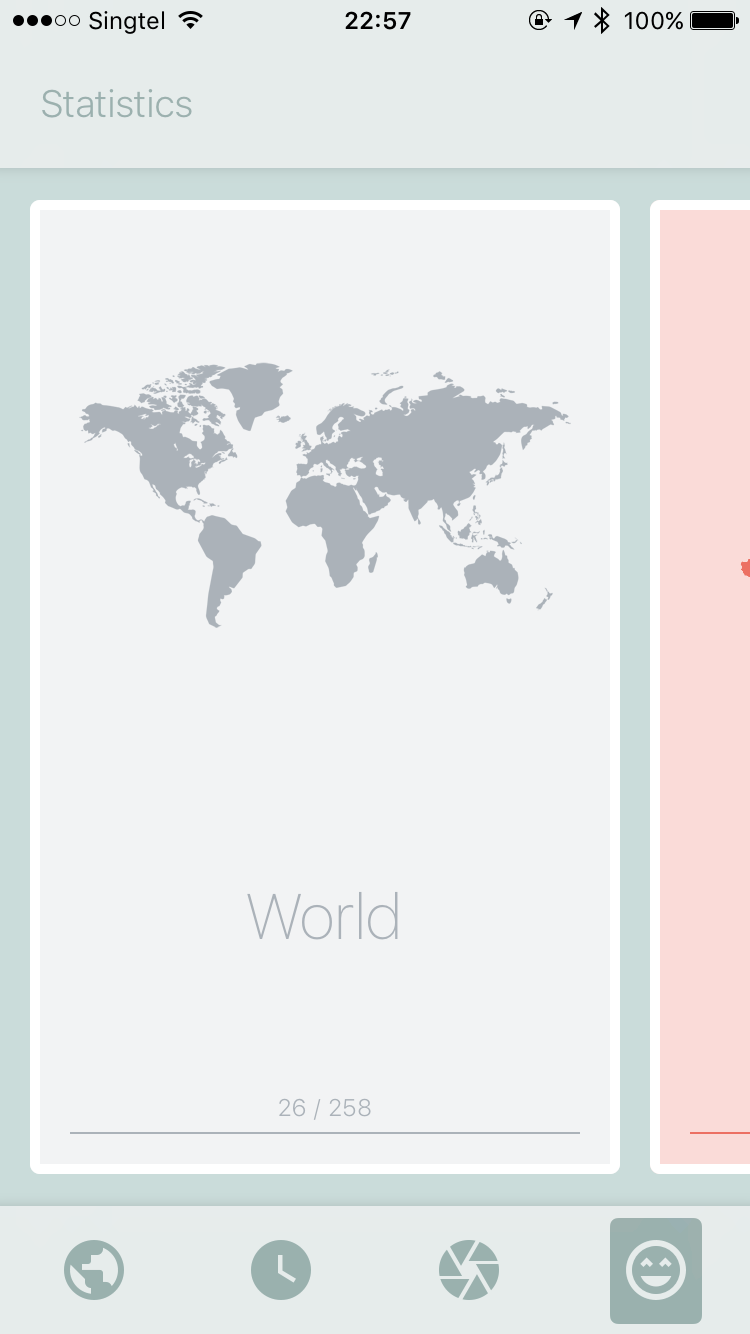
\includegraphics[width=0.32\textwidth]{4-1-7-a}
                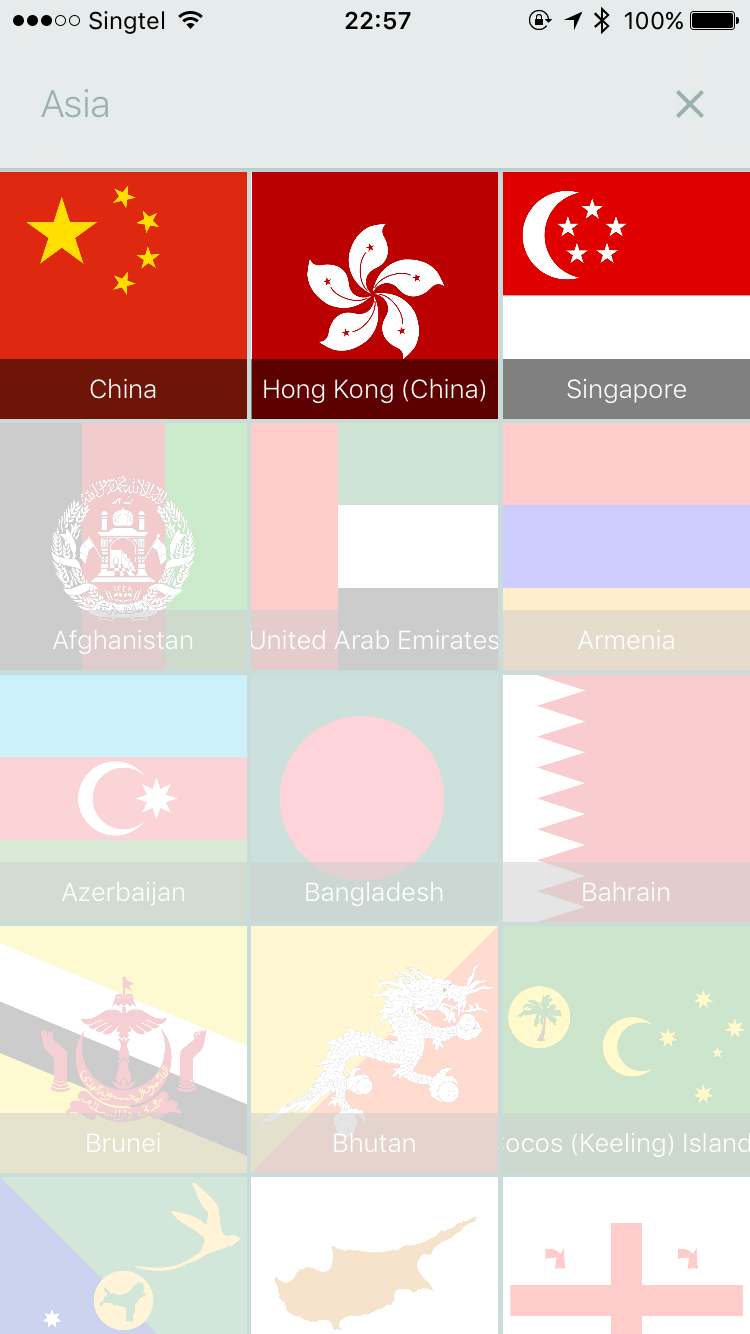
\includegraphics[width=0.32\textwidth]{4-1-7-b}
                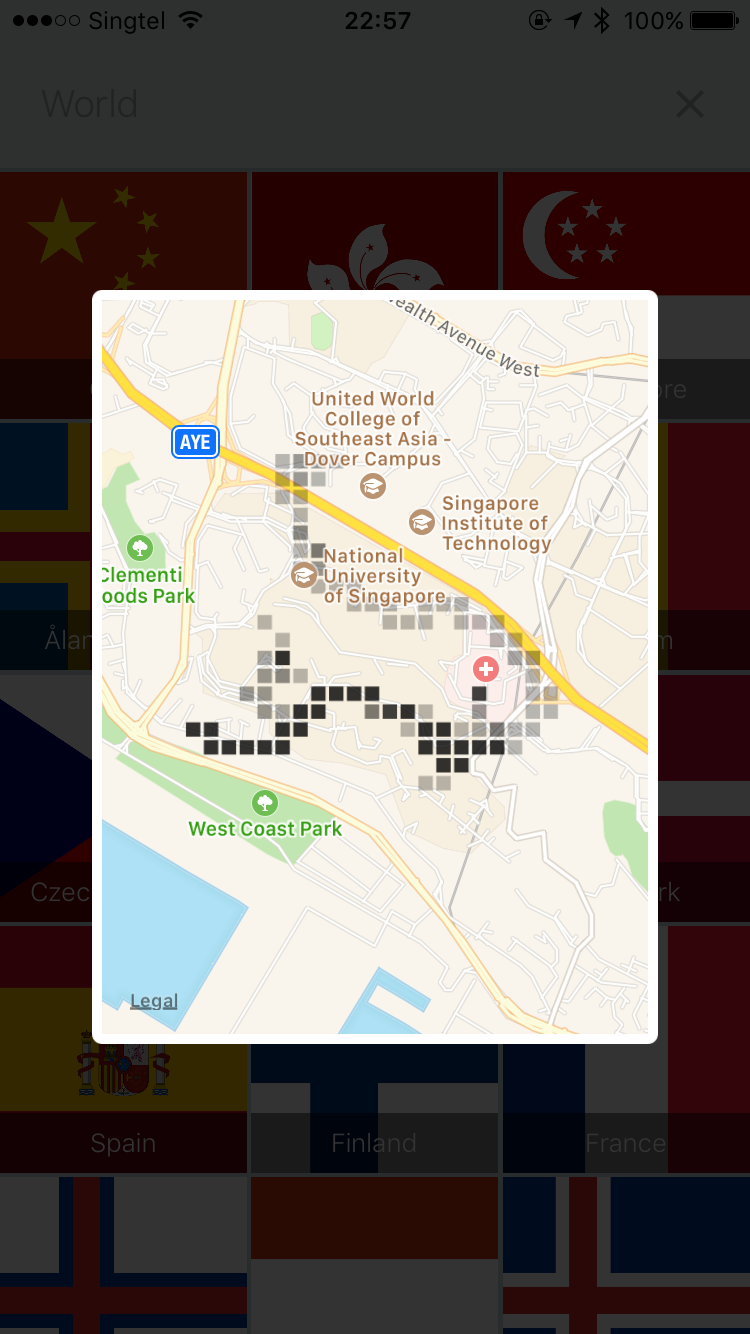
\includegraphics[width=0.32\textwidth]{4-1-7-c}
                \centering
                \caption{Check statistics of visited Countries}
                \label{fig:country-statistics}
            \end{figure}
            
            To check visited countries and the paths in a specific country, the user will need to:
            \begin{enumerate}
                \item Select the fourth tab
                \item Select world or any of the continents
                \item Browse the country list
                \item Tap on the flag of the country he or she is interested in
                \item Zoom in or out in the presented map view as he or she likes
            \end{enumerate}
            As shown in Figure \ref{fig:country-statistics}, the blacked out background in the map preview view is tappable. Tapping on it will dismiss the map preview. 
            
            \footnotesize
            Section \ref{sec:locate-photo} is written by Jinghan.
            \normalsize
    \clearpage    
    
    
    \section{Application Architecture}
        \label{sec:architecture}
        \subsection{Front-end Architecture}
        \begin{figure}[H]
            \includegraphics[width=\textwidth]{frontend-architecture}
            \centering
            \caption{Component diagram for front-end architecture}
            \label{fig:fe-classdiagram}
        \end{figure}
        
        The front-end architecture is illustrated by Figure \ref{fig:fe-classdiagram}.
        
        Since this application is following the standard Model-View-Controller architecture pattern, the main interaction in the front-end is between the view controllers and the views. The components in \textcolor{grayishblue}{grayish blue} corresponds to the basic hover tab structure and relevant protocols, which will elaborated in Section \ref{fe:fundamentals} \textit{Fundamentals}. Each of the view controllers in this application is inherited from the base class \texttt{LFViewController}, and the view controllers for the four main pages should override the delegate method from \texttt{LFHoverTabBarDataSource} in order to provide the specific control view for each pages.
        
        The view controller classes and view classes for different feature pages are labelled with different background color, the correspondence can be find with Table \ref{table:front-end-architecture-diagram}.
        
        \begin{table}
            \begin{tabular}{|p{0.5\textwidth} p{0.1\textwidth} p{0.3\textwidth}|}
                \hline
                \textbf{Feature group} & \textbf{Section} & \textbf{Color in Figure \ref{fig:fe-classdiagram}} \\
                \hline
                Fundamentals & \ref{fe:fundamentals} & \textcolor{grayishblue}{$\bullet$} Grayish blue\\
                Path history overview & \ref{fe:history-overview} & \textcolor{pink}{$\bullet$} Pink\\
                Path lists and path sharing & \ref{fe:path-lists} & \textcolor{orange}{$\bullet$} Orange\\
                Path playback & \ref{fe:path-playback} & \textcolor{yellow}{$\bullet$} Yellow\\
                Photos & \ref{fe:photos} & \textcolor{green}{$\bullet$} Green\\
                Statistics & \ref{fe:statistics} & \textcolor{cyan}{$\bullet$} Cyan\\
                Settings & \ref{fe:settings} & \textcolor{blue}{$\bullet$} Blue\\
                \hline
            \end{tabular}
            \caption{Feature correspondence for front-end architecture components}
            \label{table:front-end-architecture-diagram}
        \end{table}
        
        \subsection{Back-end Architecture}
        \begin{figure} [H]
            \includegraphics[width=\textwidth]{backend-architecture}
            \centering
            \caption{Component diagram for back-end architecture}
            \label{fig:be-classdiagram}
        \end{figure}
        
        In the back-end of this application, two databases are working together to support the persistent data storage and caching. Therefore, two different sets of models are used when dealing with data from different databases.
        
        In general, \texttt{LFPoint} and \texttt{LFPath} are the two fundamental models for the geo-location data used; wrapping \texttt{LFPath}, \texttt{LFIncomingPath} is the special path model used when handling the path shared by others. These are all subclasses of the basic \texttt{NSObject} class from iOS Foundation framework. Another set of models are the Realm Object used for caching purpose. There are three types of information we cached in the Realm database: zoom level (\texttt{LFCachedLevel}), coordinates (\texttt{LFCachedPoint}) and country information (\texttt{LFCachedCountry}).
        
        Several managers (see Service component in Figure \ref{fig:be-classdiagram}) are responsible for the communication between front-end components and the back-end database. The elaboration of each services can be found in relevant subsections of Section \ref{development-details} \textit{Development Details}.
        
        \footnotesize
            Class diagrams in section \ref{sec:architecture} are drawn by Jinghan. Texts in section \ref{sec:architecture} are written by Mingyu.
        \normalsize
    \clearpage
    
    \section{Development Details}
    \label{development-details}
    
    As the project title suggested, design and development are the two critical components of this project. In the previous section \textit{Application Architecture}, the high level structure of this application has been discussed. In this section, we will go into the details to discuss about the specific design decisions and the final implementation approach for each individual feature. The whole section is categorized into front-end part and back-end part, and the features of each part are listed accordingly. 
    
    \footnotesize
    This section is written jointly by Jinghan and Mingyu. Please refer to the individual subsections for specific attributions.
    \normalsize
            
        \subsection{Front-End Details}
        There are seven general features in terms of front-end development. The first subsection \textit{Fundamentals} will discuss the overall view hierarchy, the second subsection \textit{Map Framework} will compare the different map frameworks available and our rational behind choosing Apple MapKit as the map framework for this application, the third subsection \textit{Geo-Location Information Recording} will discuss the details of geo-location data collection, while the rest will keep the focus on different views.
            
            \subsubsection{Fundamentals} % Wang
            \label{fe:fundamentals}
            Based on the well accepted Model-View-Controller pattern, Apple has provided several standard templates for developers to organize the views in their applications. In general, developers are recommended to use these template to take advantages of the built-in optimizations. Amongst the various templates provided, we picked out the ones we may potentially make use of:
            \begin{itemize}
            \setlength\itemsep{-0.5em}
            \item master-detail application template
            \item page-based application template
            \item tabbed application template
            \end{itemize}
            
            The master-detail application template provides a convenient starting points for data driven applications where only brief data are shown in a list. Users will only view the details when they click on a specific list item. \texttt{UITableView} as the list(master) view, is the perfect fit when showing texts or simple images, but when the geo-location data come in, the list introduces too much cognitive load to the viewer. 
            
            In the page-based and tabbed application templates, there are no cognitive hassle as in master-detail template when displaying geo-location data. However, in neither of these two, there allows native accommodations for the controls. A naive solution may be in each essential view (i.e. each page in a page-based template or each tab in a tabbed template), we put the relevant controls directly on top. This will certain solve the problem, but at the cost of messing up the user's working space. Furthermore, there are possibly cases where one single control needed to be shared among different pages or tabs, but with this naive solution we will have to duplicate the codes here and there.
            
            Due to the fact that none of the templates suits our needs, we decided to implement our own view hierarchy. The customized scheme we proposed and implemented can be considered as an extension of the tabbed application template. The main difference is that in our hierarchy, the tab bar can be pulled up and reveal the control panel, where various controls are placed. The controller of each essential view will inherit a common parent view controller, which implements a protocol to delegate the data sources of the controls. When a control needs to be shared among different views, it is defined in the parent view controller. When a control is only needed in one single particular view, it is defined in the specific child view controller. In this way, we avoid the potential duplicated code. Furthermore, the customized tab bar is able to be snapped into several code-defined levels so that a control may only be shown when it is really needed by the user. Figure \ref{fig:fundamental} shows the customized tab bar in different snapping levels.
            
            \footnotesize
            Section \ref{fe:fundamentals} is written by Jinghan.
            \normalsize
            
            \begin{figure}
                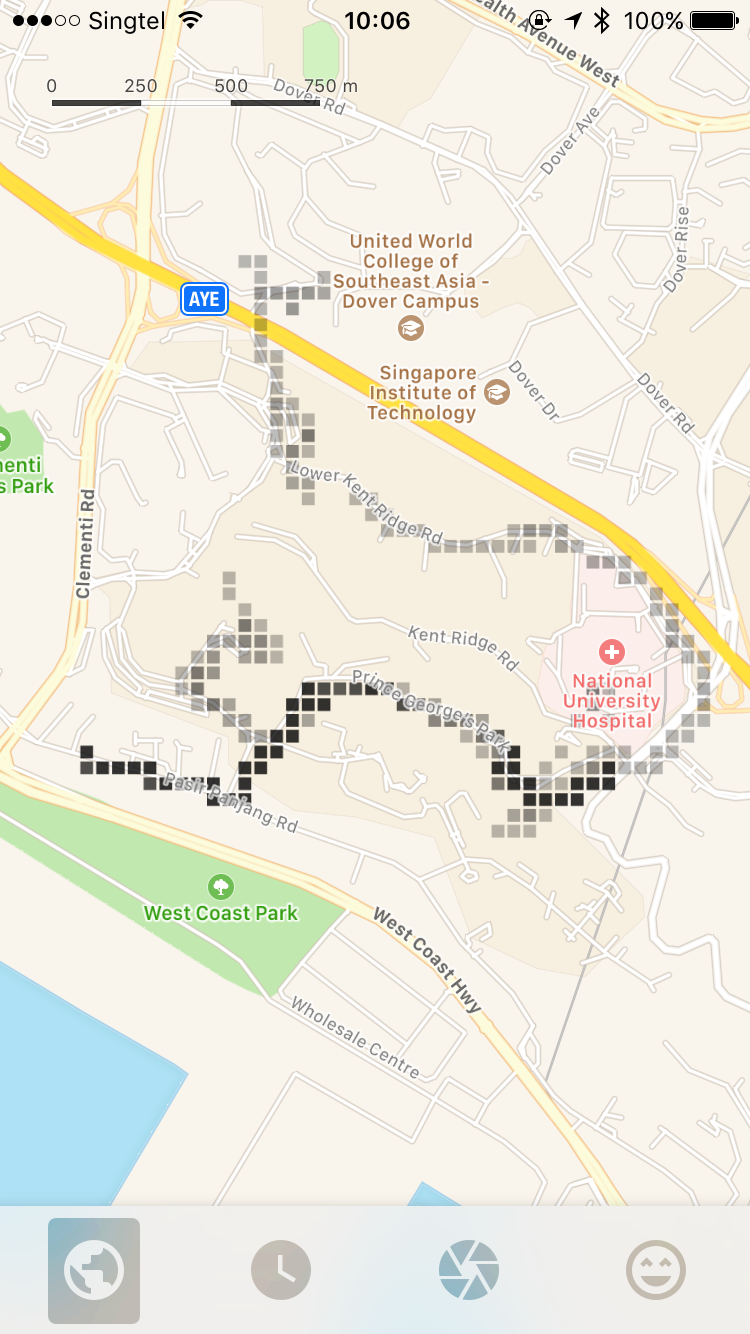
\includegraphics[width=0.32\textwidth]{4-1-1-a}
                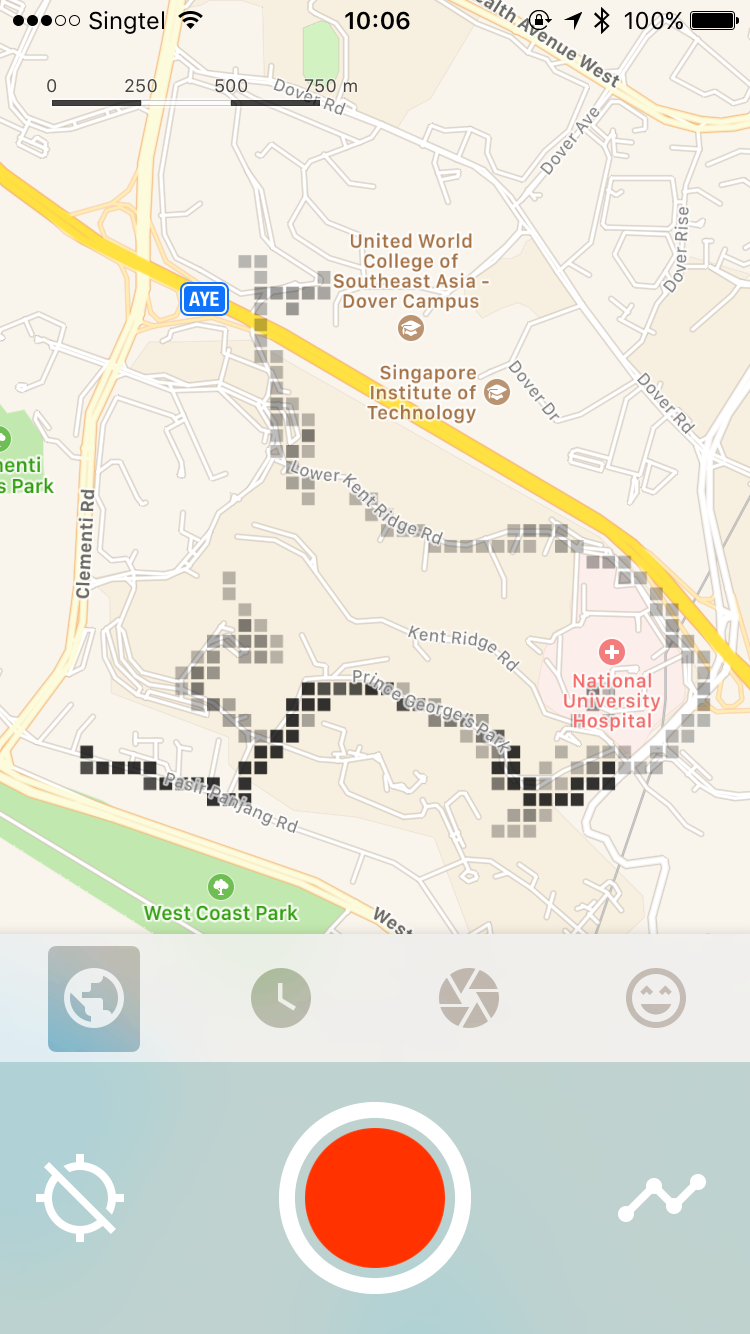
\includegraphics[width=0.32\textwidth]{4-1-1-b}
                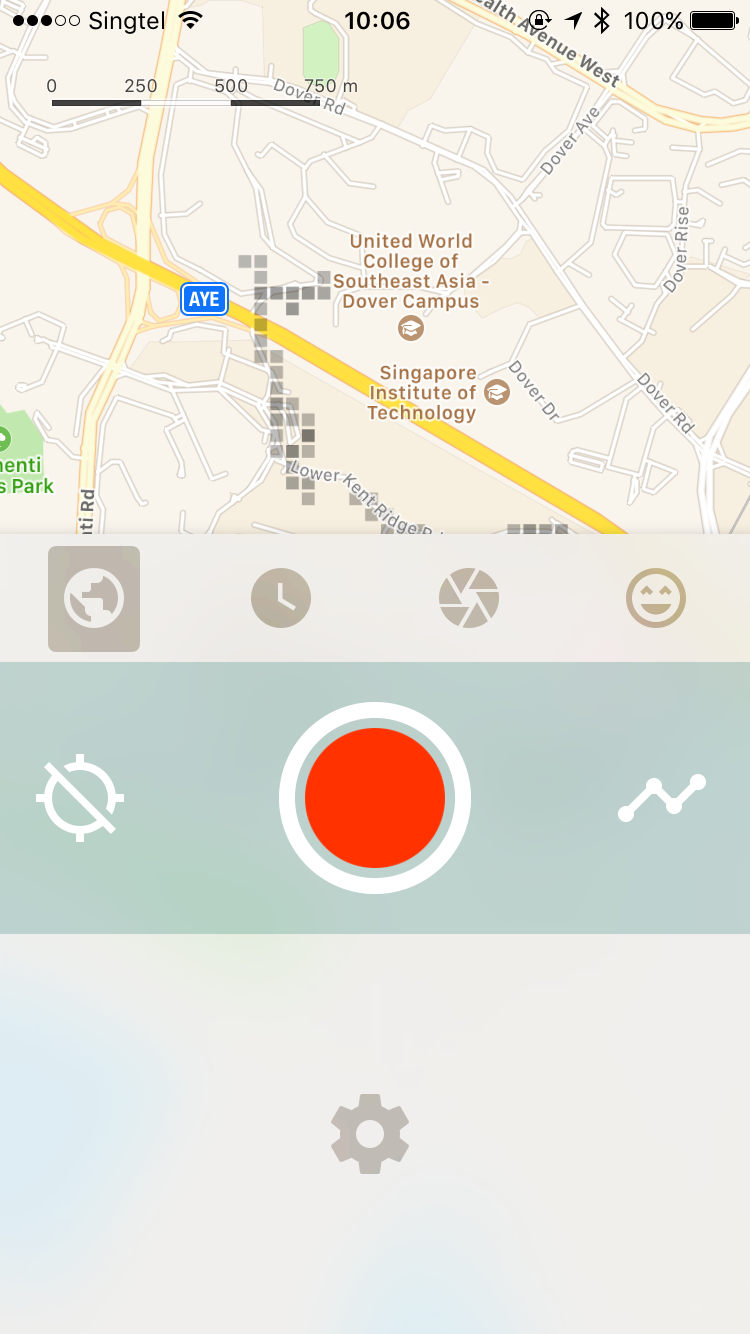
\includegraphics[width=0.32\textwidth]{4-1-1-c}
                \centering
                \caption{Customized tab bar at different snapping levels}
                \label{fig:fundamental}
            \end{figure}
            
            \subsubsection{Map Framework} % Lei/mapbox dynamic updates
                \label{fe:map-framework}
                For any application dealing with geo-location data, map is always the inherent medium to present the location information. In our initial user interface prototypes, the map is also the most important element in the entire front-end view structure. For the two core functionality pages, history overview and path playback are simply one map view with different kinds of data visualization (see Section \ref{fe:history-overview} \textit{History Overview} and Section \ref{fe:path-playback} \textit{Path Playback}). For the other secondary feature pages like photos and statistics, map also plays an important role as an essential component (see Section \ref{fe:photos} \textit{Photos} and Section \ref{fe:statistics} \textit{Statistics}).
                
                In order to display and integrate a map in the application, an appropriate map framework is needed. A map framework provides the necessary geographic information on the map and supports the basic interaction between users and the map like panning, tapping, zooming in and out etc. Usually, the map displayed from a framework can be configured with different map types. Some of the common map types includes:
                \begin{itemize}
                    \setlength\itemsep{-0.5em}
                    \item Road map: this is the default map type for most of the map frameworks (see Figure \ref{fig:map-type}, left)
                    \item Satellite map: the map is displayed as the imagery collected by the satellites operated by the governmental or non-governmental organizations (see Figure \ref{fig:map-type}, middle)
                    \item Hybrid map: this is the combination of the road map and satellite map. The map is displayed with the satellite imagery background with the labels of roads and buildings on top (see Figure \ref{fig:map-type}, right)
                \end{itemize}
                
                Satellite map gives a sense of reality since the map is composed by the real photos. When the users is interacting with the satellite map, they will have an experience as if they were looking at the earth from some aerial platform. However, when visualizing the geo-location data, there will certainly be some markers displayed on the map of the satellite imagery. The whole user interface would look pretty messy, and the path rendered will lose the visual salience thus it defeats the purpose of showing visited track on the map view. Compared to the satellite map and hybrid map, the default road map is much simpler, most of the background is painted in light plain color and there are not many map elements interfering the path viewing. For the sake of clearness, we chose the road map as the map type for this application.
                
                \begin{figure}
                    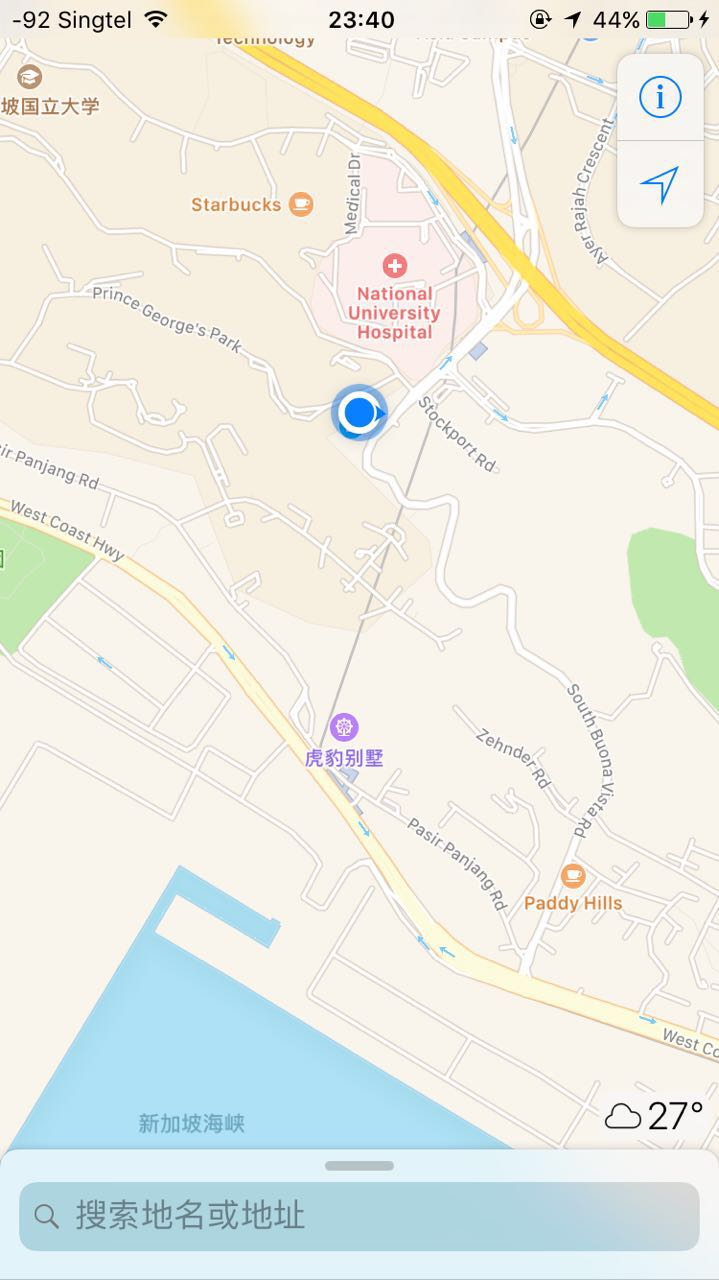
\includegraphics[width=0.32\textwidth]{4-1-2-a}
                    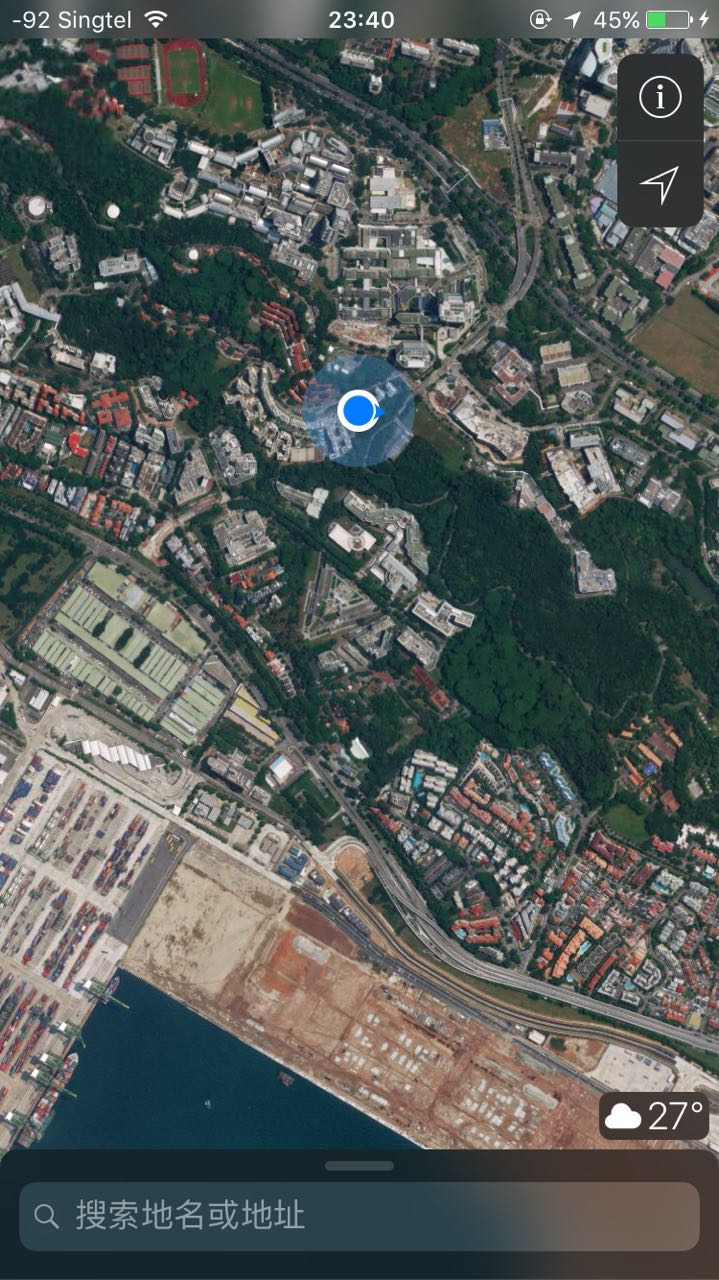
\includegraphics[width=0.32\textwidth]{4-1-2-b}
                    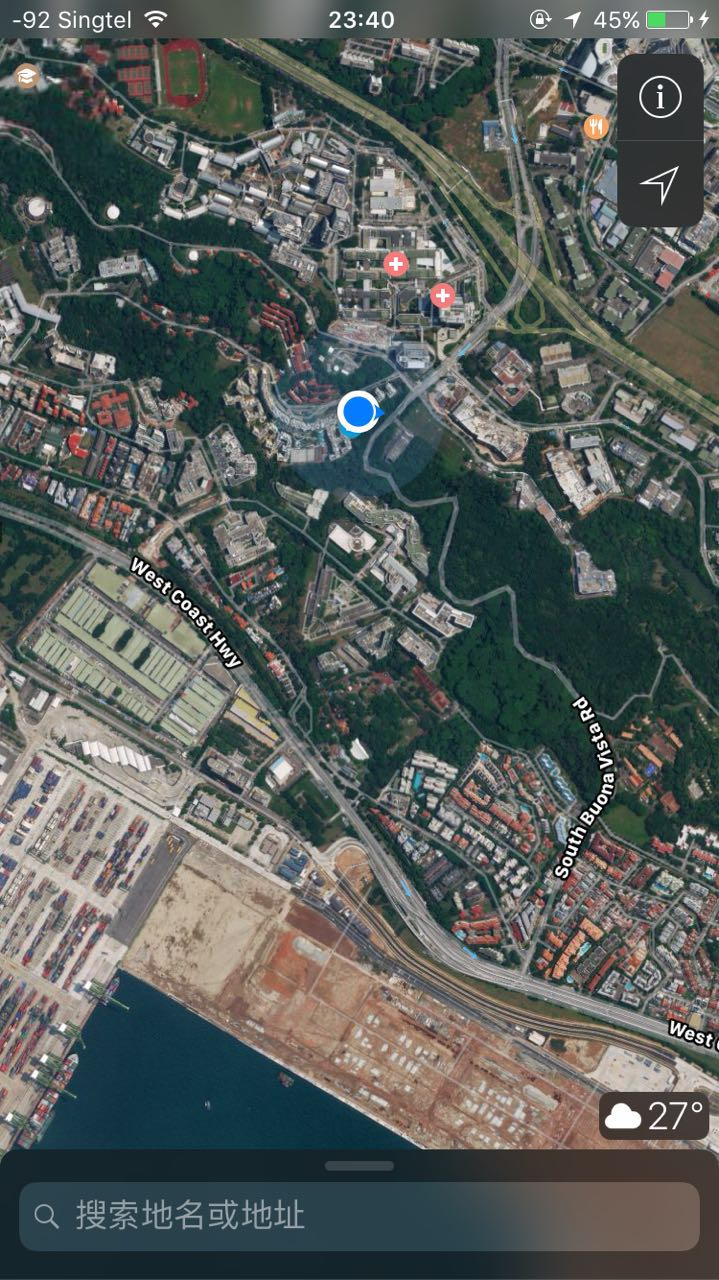
\includegraphics[width=0.32\textwidth]{4-1-2-c}
                    \centering
                    \caption{Different map type}
                    \label{fig:map-type}
                \end{figure}
                
                We have done some researches and prototypes with mainly two different map frameworks, namely Apple MapKit framework and the Mapbox framework. The rest of this section will briefly discuss these two different framework.
                
                \paragraph{Apple MapKit}
                MapKit is a native iOS SDK for displaying map in the application in the same way as the built-in map application. It has the best compatibility and integration with the other Apple framework like Core Location and Core Animation. 
                
                MapKit uses Mercator cylindrical map projection to display the map view. During the projection, the world coordinates are mapped onto the surface of a cylinder, and then unwrapped to generate a flat map. A simple conversion from longitude $\lambda$ and latitude $\phi$ to the map coordinate $x$ and $y$ can be calculated as:
                \begin{align*}
                    \begin{split}
                        x&=\lambda-\lambda_0\\
                        y&=\ln(\tan(\frac{\pi}{4}+\frac{\phi}{2}))\\
                        &=\frac{1}{2}\ln(\frac{1+\sin(\phi)}{1-\sin(\phi)})\\
                        &=\sinh^{-1}(\tan(\phi))\\
                        &=\tanh^{-1}(\sin(\phi))\\
                        &=\ln(\tan(\phi)+\sec(\phi))
                    \end{split}
                \end{align*}
                
                According to \citet{AppleMapKitUnderstandingMapGeometry}, using Mercator projection will benefit the general navigation since a straight line drawn between any two points on the map yields a course heading that can be used in actual navigation on the surface of the Earth.
                
                After the Mercator projection, the world coordinates can be converted to map points; another conversion depending on the current zoom level from map points to the actual window points need to be done. MapKit provides a set of APIs to calculate these conversions, and they are listed in Table \ref{table:mapkit-conversions}.
                
                \begin{table}
                    \begin{tabular}{ | p{2.4cm} p{2.4cm} l | }
                    \hline
                    \textbf{From} & \textbf{To} & \textbf{Conversion routines}\\
                    \hline
                    Coordinates & Points & \texttt{convertCoordinate:toPointToView:(MKMapView)}\\
                    Coordinates & Map points & \texttt{MKMapPointForCoordinate}\\
                    Map points & Coordinates & \texttt{MKCoordinateForMapPoint}\\
                    Map points & Points & \texttt{pointForMapPoint:(MKOverlayRenderer)}\\
                    Points & Coordinates & \texttt{convertPoint:toCoordinateFromView:(MKMapView)}\\
                    Points & Map Points & \texttt{mapPointForPoint:(MKOverlayRenderer)}\\
                    \hline
                    \end{tabular}
                    \caption{Map coordinate system conversion routines}
                    \label{table:mapkit-conversions}
                \end{table}
                
                The main rendering process of MapKit is tile-based, which means when the user is zooming in or out, the map is rendered as different tiles in multiple threads. The number of tiles and the size of them are based on the current zoom level. Tile-based map rendering is efficient since the rendering processes for different tiles are taken place in different threads concurrently, but it would also makes the overall rendering process looks jaggy since the user might find the map is rendered tile by tile. This is even more obvious when the user is scrolling the map or zooming in and out rapidly.
                
                While developing with MapKit, the developers can create their own renderer to display the map as desired. However, the developers have less freedom in terms of map style customization. Most likely they can only display the map in the same way as the native Apple maps; there is not even a way to hide the road label layer from the map view.
                
                Two common architectures can be implemented with MapKit framework:
                \begin{enumerate}
                    \setlength\itemsep{-0.5em}
                    \item placing \texttt{MKAnnotationView} on \texttt{MKMapView} (Figure \ref{fig:mapkit-annotation})
                    \item using \texttt{MKOverlay} and \texttt{MKOverlayRenderer} to manage the annotation overlay (Figure \ref{fig:mapkit-overlay})
                \end{enumerate}
                
                \begin{figure}
                    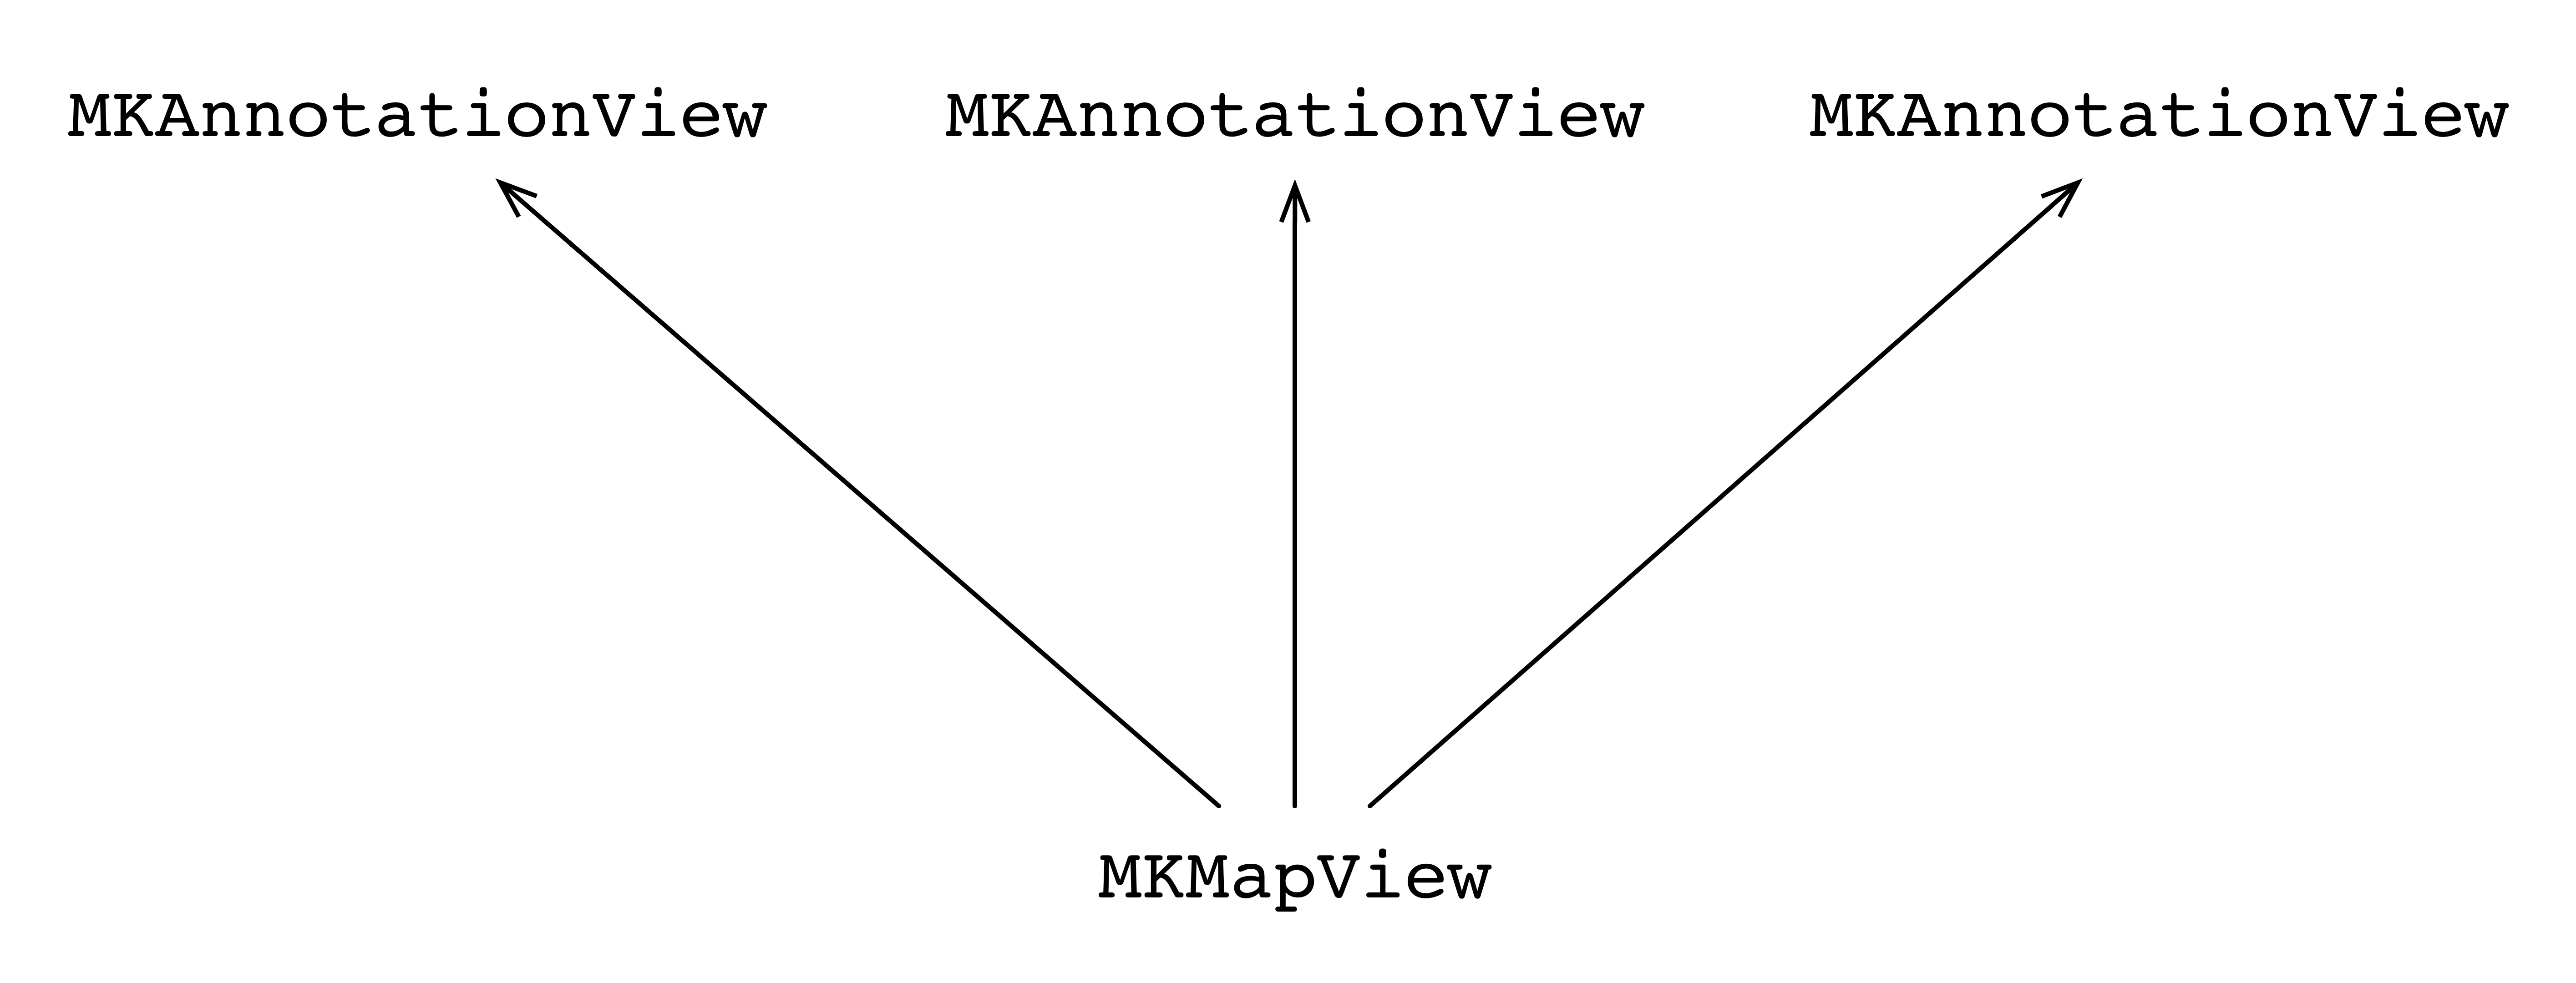
\includegraphics[width=.9\textwidth]{4-1-2-1-a}
                    \centering
                    \caption{MapKit with annotation views}
                    \label{fig:mapkit-annotation}
                \end{figure}
                
                In the first case, for each of the geo-location coordinates fetched from database, we create an instance of \texttt{MKAnnotationView} with the longitude and latitude unwrapped from the \texttt{CLLocationCoordinate2D} before rendering them on the map, and then add the \texttt{MKAnnotationView} on to the \texttt{MKMapView} by calling the \texttt{addAnnotation(annotation:MKAnnotation)} method. This is a simple yet naive way to display the data points. As the number of points increases, the performance might suffer since many annotations are directly put on the map view hierarchy. A demonstration of one prototype with this architecture is shown in the left screenshot in Figure \ref{fig:mapkit-demo}.
                
                In the second case, after fetching the geo-location coordinates from database, instead of adding \texttt{MKAnnotationView} directly to the \texttt{MKMapView}, we can create a subclass of \texttt{MKOverlay} and \texttt{MKOverlayRenderer}, and then use the customized subclass we defined of \texttt{MKOverlayRenderer} to render the visualization result from the data. With this hierarchy, the performance problem with many \texttt{MKAnnotationView} stacking in map view hierarchy is addressed, since all the coordinates data are compacted to one \texttt{MKOverlay}. Moreover, with the customization of \texttt{MKOverlayRenderer}, the path can be drawn with more variation. For instance, in the demonstration of another prototype with customized overlay renderer (the right screenshot in Figure \ref{fig:mapkit-demo}), the path can be rendered like the cleared fog in Fog of World (see Section \ref{intro:comparison:fow} \textit{Fog of World}).
                
                \begin{figure}
                    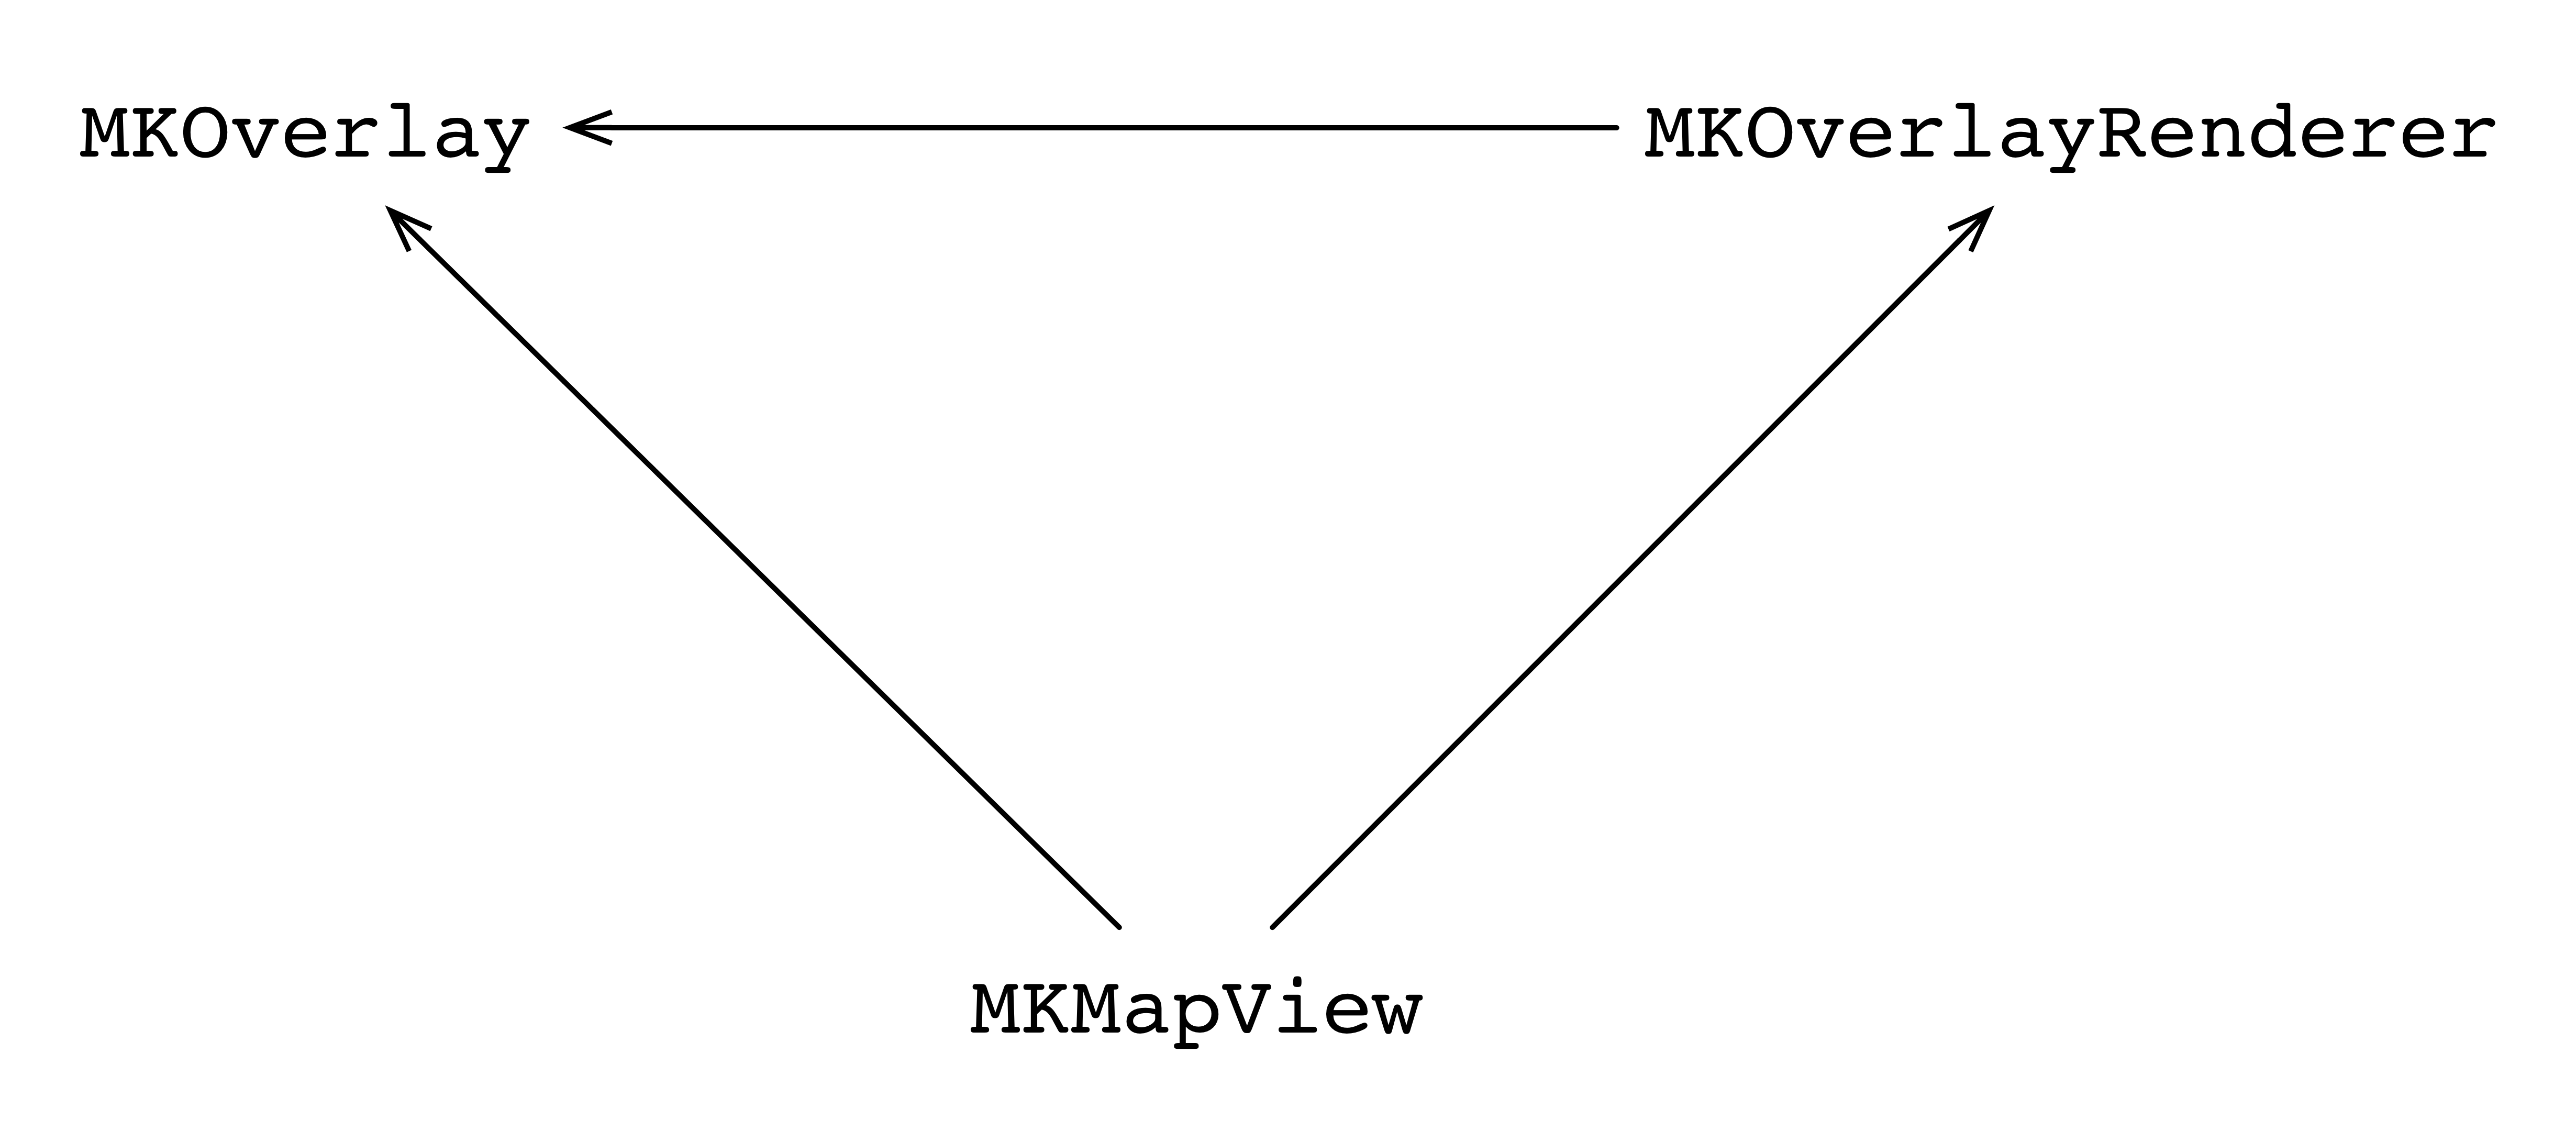
\includegraphics[width=.84\textwidth]{4-1-2-1-b}
                    \centering
                    \caption{MapKit with overlay and overlay renderer}
                    \label{fig:mapkit-overlay}
                \end{figure}
                
                \begin{figure}
                    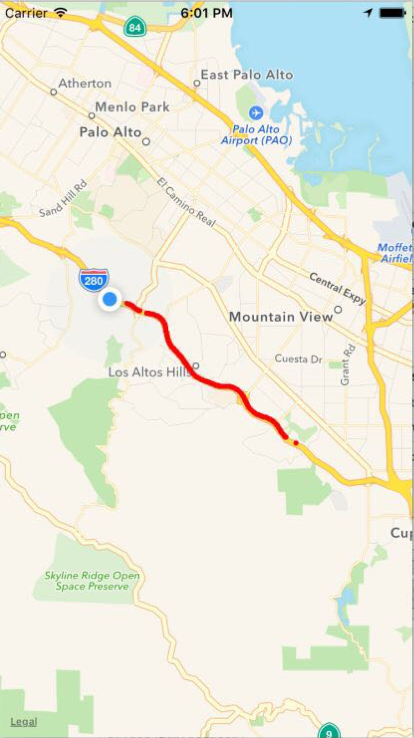
\includegraphics[width=.32\textwidth]{4-1-2-1-c}
                    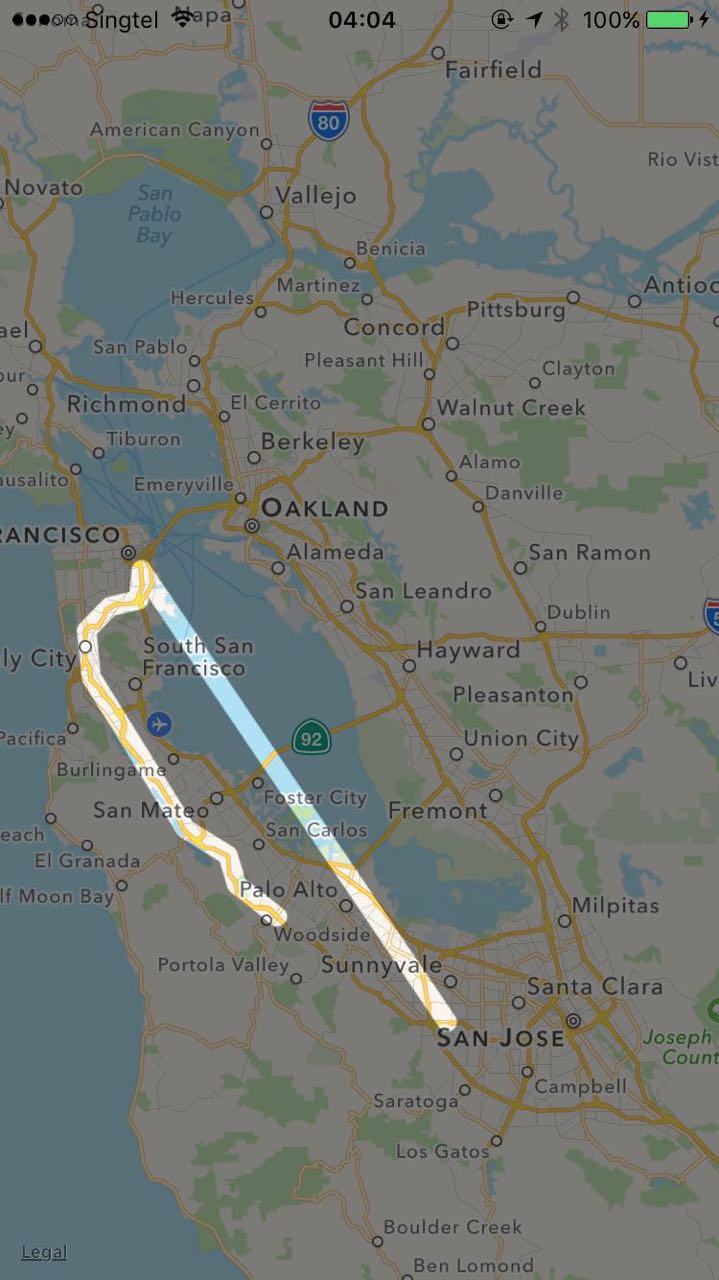
\includegraphics[width=.32\textwidth]{4-1-2-1-d}
                    \centering
                    \caption{Prototype screenshots with MapKit framework}
                    \label{fig:mapkit-demo}
                \end{figure}
                
                \paragraph{Mapbox}
                Mapbox is another map framework developed by the map service provider with the same company name ``Mapbox''. The framework is open-sourced with a productive development team. The most distinct feature of the map provided by this framework is the freedom to customize the map style. (\citet{MapboxDocumentation})
                
                Unlike the Apple MapKit framework which only allows the developer to adjust very limited customization options, Mapbox even provides a powerful map customization platform called Mapbox Studio. With the help of this platform, developers are able to make their map unique from others. Mapbox makes use of vector assets for tile rendering, therefore when the users are zooming the map in and out, they can expect the map content to be updated seamlessly (while in Apple MapKit the tiles need to be updated since they are not vector tiles).
                
                Although Mapbox provides thorough customization freedom for map styling, it limits developers' capability to customize the rendering process. That is to say, the developers will not be able to create their own map renderers as in MapKit. Instead, the rendering work will be delegated to the Mapbox framework to complete.
                
                \begin{figure}
                    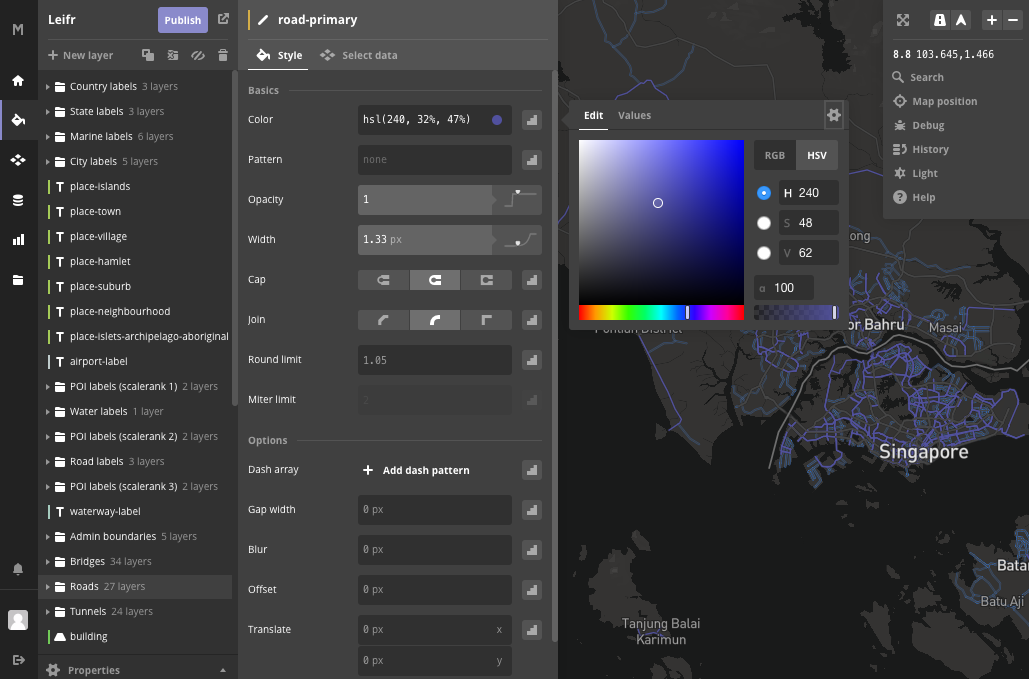
\includegraphics[width=.8\textwidth]{4-1-2-2-c}
                    \centering
                    \caption{Mapbox Studio}
                    \label{fig:mapbox-studio}
                \end{figure}
                
                Three common architectures can be implemented with Mapbox framework:
                \begin{enumerate}
                    \setlength\itemsep{-0.5em}
                    \item placing \texttt{MGLAnnotation} on \texttt{MGLMapView} (Figure \ref{fig:mapbox-annotation})
                    \item using \texttt{MGLOverlay} to manage the annotations (Figure \ref{fig:mapbox-overlay})
                    \item using the ``datasource-layer'' model to manage the annotations with geo-location data (Figure \ref{fig:mapbox-datasource})
                \end{enumerate}
                
                \begin{figure}
                    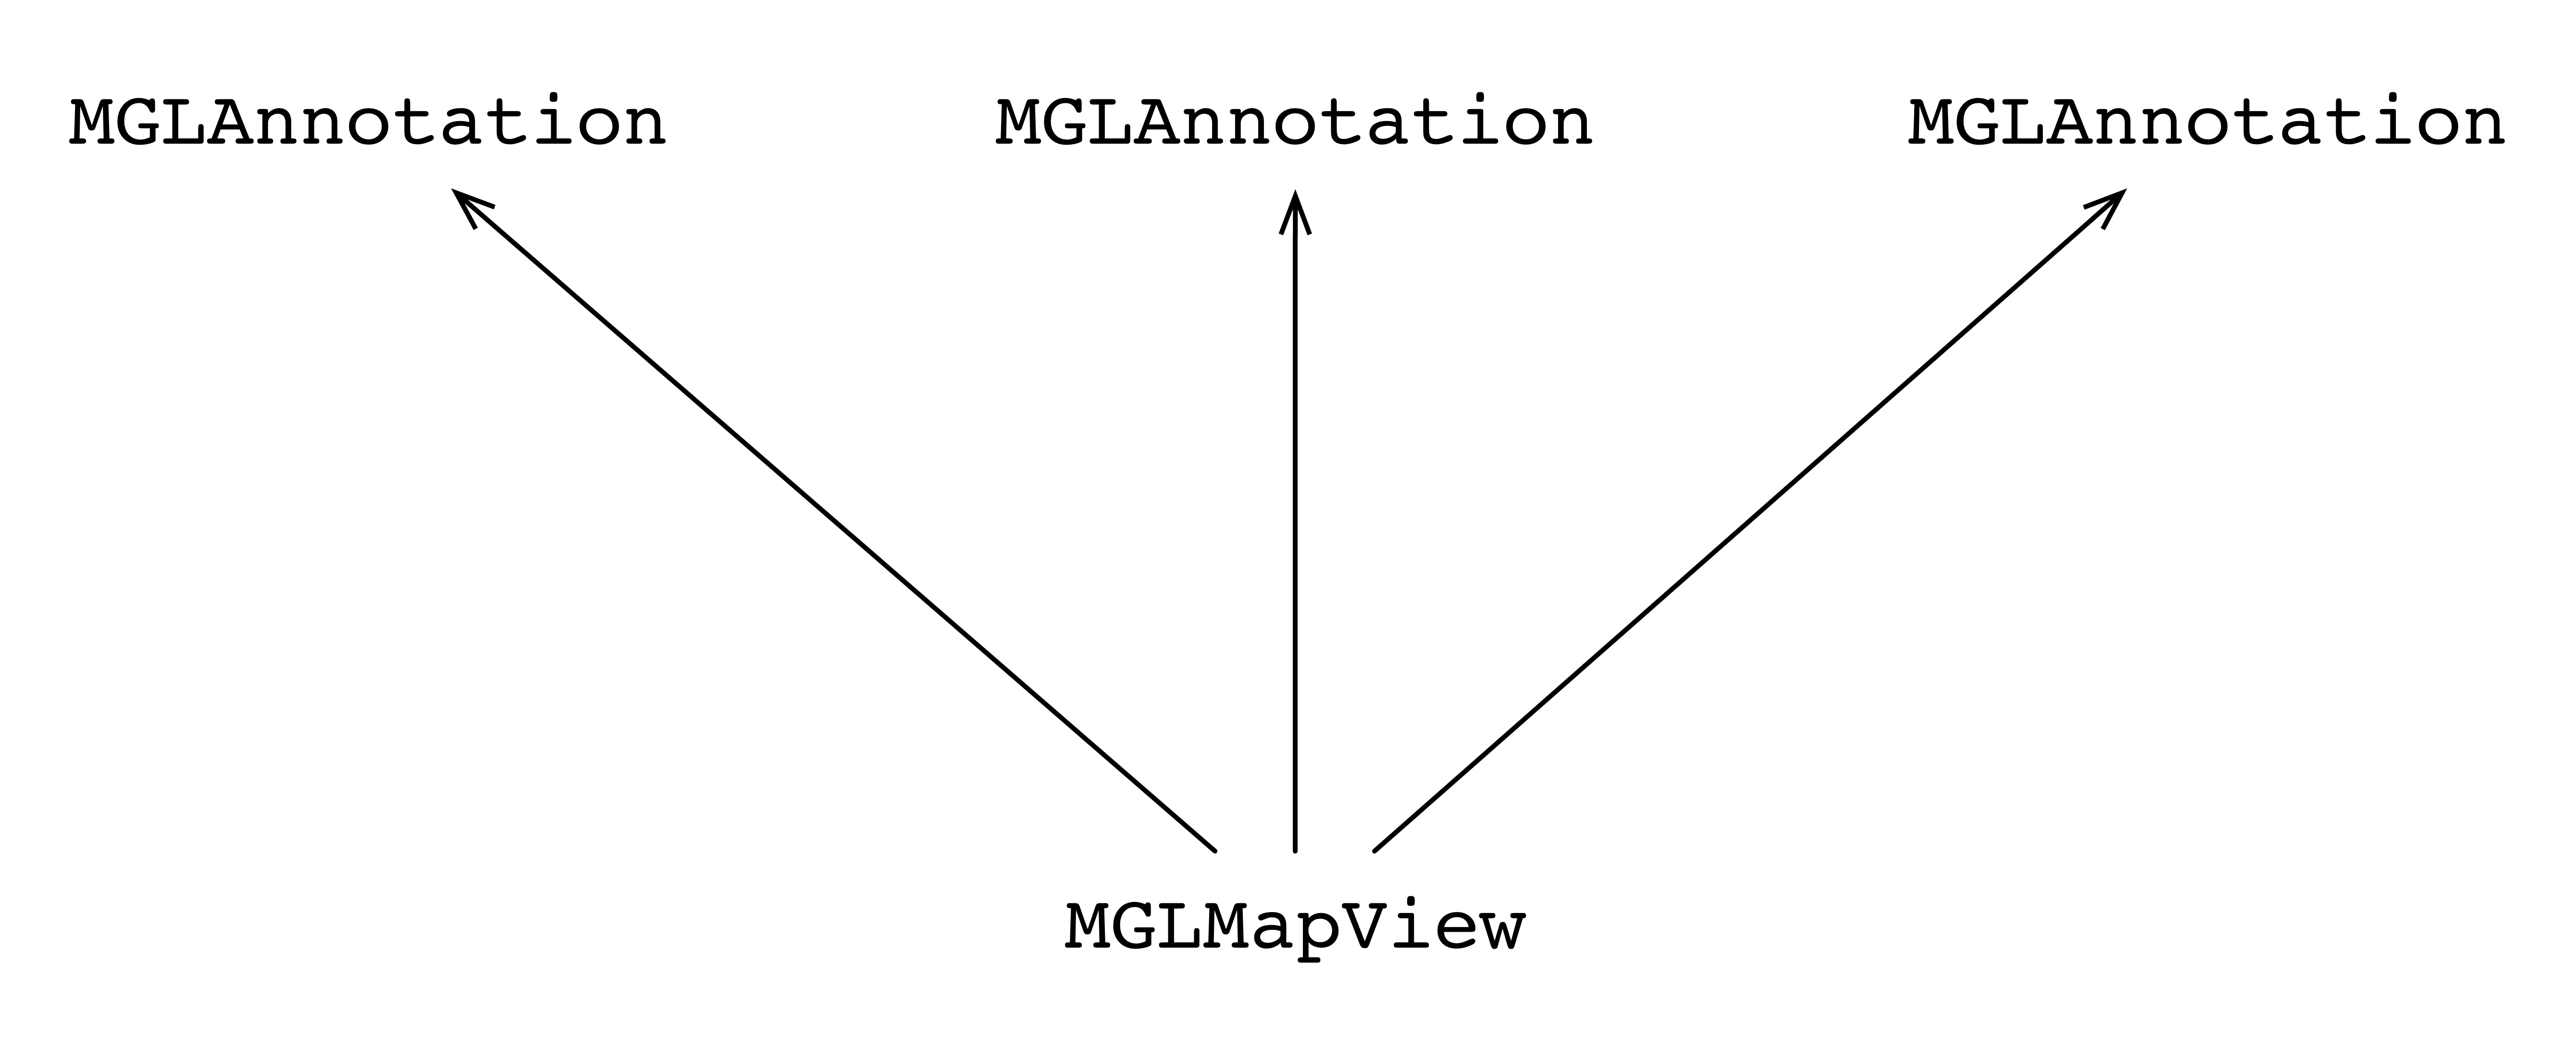
\includegraphics[width=\textwidth]{4-1-2-2-a}
                    \centering
                    \caption{Mapbox with annotation views}
                    \label{fig:mapbox-annotation}
                \end{figure}
                
                The first approach is similar to the naive way of putting annotations on MapKit's mapview, except the \texttt{MKAnnotationView} and \texttt{MKMapView} are replaced by \texttt{MGLAnnotation} and \texttt{MGLMapView}, and the method for adding \texttt{MGLAnnotation} is \texttt{addAnnotation(annotation: MGLAnnotation}. During prototyping, \texttt{MGLPointAnnotation}, which is a concrete class conforms to \texttt{MGLAnnotation} protocol, is used for rendering the geo-location points. The appearance of the \texttt{MGLAnnotation} can be configured by overriding the following two delegate methods from \texttt{MGLMapViewDelegate}:
                \begin{enumerate}
                    \setlength\itemsep{-0.5em}
                    \item \texttt{mapView(mapView:imageForAnnotation:)}
                    \item \texttt{mapView(mapView:viewForAnnotation:)}
                \end{enumerate}
                
                These two methods manage the customized appearance of the \texttt{MGLAnnotation}. During the implementation of the overridden methods from \texttt{MGLMapViewDelegate}, if one of these two methods is not implemented or the return value is set to \texttt{nil}, Mapbox renderer will use the other as the customization method. If neither of these two methods are implemented or they all return \texttt{nil}, Mapbox will use the default annotation as the annotation appearance.
                
                There are a few differences between them which we need to consider this when choosing the appropriate configuration approach. Configuring annotation images will make the annotations shown as static images. This allows the developer to design the marker with other tools and save it as a separate image file. On the other hand, the second approach is returning a view object for the annotation to be rendered. In this case, the view will be drawn programmatically in the subclass of \texttt{MGLAnnotationView}. Rendering annotation markers as annotation view will make them more compatible with Apple's native UIKit, Core Animation and some other Cocoa Touch frameworks, which enhances the interaction between the user and the system. However, the trade-off is higher CPU usage and longer drawing process than using static image. We performed a benchmarking experiment using Xcode Instruments tool, which adds 13,000 markers on the map, and then do some basic operation like panning and zooming. The result can be found in Figure \ref{fig:mapbox-performance-image} and \ref{fig:mapbox-performance-view}. The conclusion of this experiment is pretty straightforward: it proves that using static images as annotation markers yields better performance.
                
                \begin{figure}
                    \includegraphics[width=.8\textwidth]{4-1-2-2-x}
                    \centering
                    \caption{CPU usage for rendering 13,000 markers in Mapbox with annotation images}
                    \label{fig:mapbox-performance-image}
                \end{figure}
                
                \begin{figure}
                    \includegraphics[width=.8\textwidth]{4-1-2-2-y}
                    \centering
                    \caption{CPU usage for rendering 13,000 markers in Mapbox with annotation views}
                    \label{fig:mapbox-performance-view}
                \end{figure}
                
                Continuing the discussion of Mapbox integration approach, Figure \ref{fig:mapbox-overlay} shows an improved version which is similar to Figure \ref{fig:mapkit-overlay}. The ideas behind are the same: add one overlay on top of the map view and render the annotations in the overlay layer instead of adding too many annotation on the map view directly. Although the previous paragraph mentioned that using static image can alleviate some memory pressure, mobile devices are still not able to afford the great number of annotations displayed at the same time. Since our application is dealing with many geo-location points in one recorded path, it is better to have the overlay to manage differnt points instead.
                
                \begin{figure}
                    \includegraphics[width=\textwidth]{4-1-2-2-d}
                    \centering
                    \caption{Mapbox with overlay}
                    \label{fig:mapbox-overlay}
                \end{figure}
                
                \begin{figure}
                    \includegraphics[width=.88\textwidth]{4-1-2-2-b}
                    \centering
                    \caption{Mapbox with \texttt{MGLGeoJSONSource}}
                    \label{fig:mapbox-datasource}
                \end{figure}
                
                In the previous approaches, the general flow of fetching and displaying the points are similar, which is querying database to get the data, converting the data to a list of \texttt{CLLocationCoordinate2D}, creating annotations with the coordinates information, and finally displaying it on the map. Mapbox provides another way to achieve the same goal: using \texttt{MGLStyleLayer} to manage rendering and \texttt{MGLSource} to manage data source. More specifically, in order to render the visited path, we can encode the geographic information from database into GeoJSON format, create \texttt{MGLGeoJSONSource} with the encoded data, associate it with an \texttt{MGLCircleStyleLayer}, and finally add these two components to the map view together by calling \texttt{addLayer(layer:)} and \texttt{addSource(source:)} method from the \texttt{MGLMapView}'s \texttt{style} attribute. One advantage of this approach is that it simplifies the integration process between map framework and the backend data. With \texttt{MGLGeoJSONSource}, the GeoJSON data can be directly generated from the SpatiaLite query (see Section \ref{db:spatialite}, \textit{SpatiaLite}) with some format tuning from \texttt{LFGeoJSONManager}. It then can be bound to the map view and render the visualization outcome. Unfortuantely, the Mapbox support for rendering with \texttt{MGLGeoJSONSource} was the new feature by the time we were doing the technology study and research. Until we finished the prototype and decision phase, it's still under development and the feature was only partially available in the alpha version of 3.4.0, and some key features we required in the application, such as dynamic update of GeoJSON source when a new point is recorded, is not supported.
                
                The screenshots of path rendering using Mapbox framework are shown in Figure \ref{fig:mapbox-screenshots}. The one on the left is using default annotaion marker, while the one on the right is using \texttt{MGLGeoJSONSource} with \texttt{MGLCircleStyleLayer}.
                
                \begin{figure}
                    \includegraphics[width=.32\textwidth]{4-1-2-2-i}
                    \includegraphics[width=.32\textwidth]{4-1-2-2-j}
                    \centering
                    \caption{Rendering geo-location data with Mapbox framework}
                    \label{fig:mapbox-screenshots}
                \end{figure}
                
                \paragraph{Map Framework Decision}
                \label{fe:map-framework-decision}
                To conclude the discussion in the previous paragraphs, here is a table of all the advantages and disadvantages of MapKit and Mapbox frameworks.
                
                \begin{table}
                    \begin{tabular}{|p{0.45\textwidth}|p{0.45\textwidth}|}
                        \hline
                        \multicolumn{2}{|c|}{\textbf{Advantages}} \\
                        \hline
                        \textbf{MapKit} & \textbf{Mapbox} \\
                        \hline
                        Well documented                 & Well documented\\
                        Native stable SDK               & Active community\\
                        Best compatibility              & GeoJSON source support \\
                        No extra library needed         & Open-sourced, fast-faced \\
                        Customizable rendering process  & Highly customizable style \\
                        Efficient tile-based rendering  & Vector tile, smooth loading \\
                        \hline
                        \hline
                        \multicolumn{2}{|c|}{\textbf{Disadvantages}} \\
                        \hline
                        \textbf{MapKit} & \textbf{Mapbox} \\
                        \hline
                        Jagged tile loading             & No control over renderer \\
                        Less customizable style         & Unofficial, compatibility problems \\
                                                        & Less flexible to manage dynamic data \\
                        \hline
                    \end{tabular}
                    \caption{Map frameworks comparison}
                    \label{table:map-framework-comparison}
                \end{table}
                
                To fully support our proposed features for this application, there are several criteria we need to consider when choosing the appropriate framework:
                \begin{itemize}
                    \setlength\itemsep{-0.5em}
                    \item The map framework should be stable to use.
                    \item The map framework should provide the rendering support for visualizing the geo-location data.
                    \item The map framework should allow the implementation of annotation animation for the path playback feature.
                    \item The map displayed should be simple, clear, and clean without too much interference with the rendered path.
                \end{itemize}
                
                Judging from the advantages and disadvantages of these two frameworks and the how well the framework suits our features, we have decided to use Apple MapKit as the map framework in this application. However, since Mapbox is under such a productive and aggressive development, we will keep following the updates from this framework. We might consider supportting both frameworks in the future if the compatibility problems between Mapbox and our desired features are solved in the future.
                
                \footnotesize
                Section \ref{fe:map-framework} is written by Mingyu.
                \normalsize
            
            \subsubsection{Geo-Location Information Recording} %
                \label{fe:geolocation-information-recording}
                The core features of this application are based on the data recorded by user. In the application, a singleton manager \texttt{LFGeoRecordManager} is dedicated to all the services involving geo-location recording. When the user switches on the recording, the flag \texttt{isRecording} in \texttt{LFGeoRecordManager} will be set to \texttt{true}. This flag is checked in several places like the \texttt{LFHistoryViewController} (see Section \ref{fe:history-overview}) and \texttt{AppDelegate}. In the latter case, the flag checking happens when \texttt{CLLocationManager} detects an update of the current location with the delegate method \texttt{locationManager(manager: didUpdateLocations locations:)}: if the flag is on, \texttt{LFGeoRecordManager} encapsulates the coordinate of the new location and the time information into an abstracted model \texttt{LFPoint} and then appends it to a buffer path. The rational behind is that it takes significantly longer time to access the database than manipulating a in-memory variable. By buffering the incoming geo-location information and flushing the path into database regularly, frequent database accesses are avoided. The interval between each flush is set to 600 seconds. The user can also perform manual flushing in the settings page (see \ref{fe:settings} \textit{Settings}). Once the recording is stopped by the user, the current buffer path will be flushed as well.
                
                In \texttt{LFGeoRecordManager}, a mutex is applied to ensure that appending a point and flushing the existing points won't happen simultaneously.
                
                \footnotesize
                Section \ref{fe:geolocation-information-recording} is written by Mingyu.
                \normalsize
            
            \subsubsection{History Overview} % Wang
            \label{fe:history-overview}
            
            History Overview is the first view the user will see after they open the application. It shows aggregated records of all places the user have been to in a pixel-style overlay. While the user zooming in and out, different levels of details will be loaded dynamically according the zoom level of the map. This is shown in Figure \ref{fig:history-overview}.
            
            \begin{figure}
                \includegraphics[width=0.32\textwidth]{4-1-4-a}
                \includegraphics[width=0.32\textwidth]{4-1-4-b}
                \includegraphics[width=0.32\textwidth]{4-1-4-c}
                \centering
                \caption{Different levels of details at different zoom level}
                \label{fig:history-overview}
            \end{figure}
            
            As mentioned in section \ref{fe:map-framework-decision}, we will take the combination of \texttt{MapKit}, \texttt{MKOverlay} and \texttt{MKOverlayRenderer} to render our geo-location data. When the map renders a tile for a specific region, the rendering process include six steps:
            
            \begin{enumerate}
                \item Get all the overlays of the \texttt{MKMapView}.
                \item Test the target region against the \texttt{boundingMapRect} property of the overlay, and only keep the overlays that lie partially or completely in the target region.
                \item The \texttt{MKMapView} call its delegate to get the renderers for the shortlisted overlays.
                \item The method \texttt{canDraw(mapRect:zoomScale:in:)} of the renderer is called. This method returns a boolean indicates whether the renderer is ready for the drawing.
                \item If the renderer is ready, the method \texttt{draw(mapRect:zoomScale:in:)} of the renderer is called and the renderer draws the customized contents onto a provided \texttt{CGContext} instance.
                \item The \texttt{CGContext} instance is used to render the drawing on screen.
            \end{enumerate}
            
            The key step in this process is step 5, where our customized renderer draws contents onto the \texttt{CGContext} according to the \texttt{mapRect} and \texttt{zoomScale} passed in. The \texttt{mapRect} property represents the rectangular region of the tile on the 2D map (i.e. the outcome of Mercator projection as mentioned in section \ref{fe:map-framework}). \texttt{zoomScale} represents the degree of details the map is in. It is a \texttt{CGFloat}, ranges from $2^{-17}$ (least detailed level) to $2^{1}$ (most detailed level). 
            
            A more popular and intuitive descriptor for the degree of details is zoom level, which is a non-zero integer. Zoom level 0 gives the world in a single tile and every time the level is incremented by 1, each of the tiles is split into 4 (2$\times$2). The correlation between zoom level ($l$) and zoom scale ($z$) is:
            \begin{equation*}
                l = 20 + \log(z)
            \end{equation*}
            
            Across the project, zoom level and zoom scale are used interchangeably according to the situation. 
            
            After getting the paramters from the caller, the \texttt{draw(mapRect:zoomScale:in:)} method will draw the overlay in the following steps:
            
            \begin{enumerate}
                \item Query \texttt{LFCachedDatabaseManager} with the specific \texttt{mapRect} and \texttt{zoomScale}, and get a list of \texttt{LFCachedPoint}s.
                \item For each \texttt{LFCachedPoint}, construct a \texttt{MKMapPoint} instance with the \texttt{x} and \texttt{y} value stored inside.
                \item Convert the \texttt{MKMapPoint} to a \texttt{CGPoint} using the method \texttt{point(mapPoint:)}.
                \item Calculate the drawing size for each point according to current \texttt{zoomScale}.
                \item Calculate the drawing rect with the size from step 4 and the point from step 3.
                \item Calculate color of the point according to its \texttt
                {count} property. \texttt{count} of a point represents the number of times the point has been visited. A larger \texttt{count} will lead to a higher alpha value.
                \item Fill the rect from step 5 with the color from step 6
            \end{enumerate}
            
            One thing that worth noting is that for each point, the alpha value of the color is not necessarily in a linear function with the \texttt{count} of that point. This is based on the consideration that people tend to stay at one place (his or her home, company or school) most of the time. If the alpha calculation follows a linear function strictly, the outcome will be that several points are completely opaque, while the others are almost completely transparent and can hardly be seen. To address this issue, we set a lower (0.2) and a upper bound (0.8) for the alpha value as well as a ``count cap'' for the alpha change. Then \texttt{count} values from 0 to the count cap maps to the possible alpha range. In this way, a relatively aesthetic appearance of the overlay is always guaranteed.
            
            \footnotesize
            Section \ref{fe:history-overview} is written by Jinghan.
            \normalsize
            
            
            \subsubsection{Path Lists} % Wang
            \label{fe:path-lists}
            
            In path list views, users may view, delete and share the paths of their own and the paths from their friends, as shown in Figure \ref{fig:path-lists}. There are two view controllers presenting similar views but fetching data from different back-end components. \texttt{LFMyTrackViewController} shows the user's own paths, and it fetches paths from the main database through the facade of \texttt{LFDatabaseManager}. On the other hand, \texttt{LFInboxViewController} shows the paths from friends, and fetches the data directly from local file systems through the facade of \texttt{LFLocalFileManager}. The differences between these two back-end components and the rational behind will be discussed in section \ref{db:direct-files}.
            
            \begin{figure}
                \includegraphics[width=0.32\textwidth]{4-1-5-a}
                \includegraphics[width=0.32\textwidth]{4-1-5-b}
                \includegraphics[width=0.32\textwidth]{4-1-5-c}
                \centering
                \caption{Path list views}
                \label{fig:path-lists}
            \end{figure}
            
            In \texttt{LFMyTrackViewController}, paths are loaded on batches instead of being loaded all at once to reduce the latency when the view is presented. There is no such mechanism in \texttt{LFInboxViewController} because the incoming paths from friends are considered sparse and manageable.
            
            In either view, sliding a cell to the left will reveal two buttons, as shown in the middle picture of Figure \ref{fig:path-lists}. This behavior is achieved through implementing the protocol method \texttt{tableView(tableView:editActionsForRowAt:)} in  \texttt{UITableViewDelegate}. In this method, we can define the buttons and specify the corresponding actions when a user taps on it.
            
            When the sharing button is tapped, the \textit{system file sharing prompt} will be popped out, and the user will then be able to select the application to which he or she wants Leifr to export. In Figure \ref{fig:path-share}, the left and middle picture show the export process. In another application (probably on another device), as the right picture of Figure \ref{fig:path-share} shows, Leifr will appears in the sharing prompt as the first option to handle the \texttt{.leifr} files.
            
            \begin{figure}
                \includegraphics[width=0.32\textwidth]{4-1-5-d}
                \includegraphics[width=0.32\textwidth]{4-1-5-e}
                \includegraphics[width=0.32\textwidth]{4-1-5-f}
                \centering
                \caption{Path export and import}
                \label{fig:path-share}
            \end{figure}
            
            The path exporting described above is achieved in three steps: 
            
            \begin{enumerate}
                \item Archive a path into a file. This is done through the implementation of \texttt{NSCoding} protocol, the details of which will be discussed in section \ref{db:direct-files}.
                \item Initialize an instance of \texttt{UIDocumentInteractionController} with the file's URL.
                \item Present the \texttt{UIDocumentInteractionController} to pop the system sharing prompt.
            \end{enumerate}
            
            After implementing export, we still need to associate our app with the file extension in the system so that it can be recognized as a handler of that particular type of files (\texttt{.leifr} files). This is done by adding in the \texttt{CFBundleDocumentTypes} entry in the application specification file \texttt{info.plist}.
            
            \footnotesize
            Section \ref{fe:path-lists} is written by Jinghan.
            \normalsize
            
            \subsubsection{Path Playback} % Lei 
                \label{fe:path-playback}
                In the path playback page, there are two possible states: the state when there are some paths selected to play and the state when there isn't any path selected. Before the user selects any path, the control panel for this page will only contain a calendar icon (see Figure \ref{fig:playback-tab}, left). If some paths have been selected, but the animation has not started, there will be an extra play button in the control panel (see Figure \ref{fig:playback-tab}, middle). If the user initiates the animation, the play button will be replaced by a pause/resume button. Additionally, a stop button will also be added into the control panel to support the full playback control (see Figure \ref{fig:playback-tab}, right).
                
                \begin{figure}
                    \includegraphics[width=0.32\textwidth]{4-1-6-a-real}
                    \includegraphics[width=0.32\textwidth]{4-1-6-b-real}
                    \includegraphics[width=0.32\textwidth]{4-1-6-c-real}
                    \centering
                    \caption{Path playback view with different tab bar content}
                    \label{fig:playback-tab}
                \end{figure}
                
                There are two ways of selecting paths: on the one hand, the path can be selected from the path lists. When a certain row in those two list is tapped, \texttt{LFPathsPlayingManager} will create an \texttt{LFPath} array with only one path inside. On the other hand, if the user selected multiple paths from the calendar by specifying the starting date, \texttt{LFPathsPlayingManager} will load an \texttt{LFPath} array with only many paths inside. For each \texttt{LFPath} array, a \texttt{LFPathPlayingManager} will be created and be in charge of the playing management of that particular array of \texttt{LFPath}. The detailed demonstration of path selection can be found in Section \ref{sec:select-path}.
                
                Currently the property \texttt{paths} in \texttt{LFPathsPlayingManger} (which is of the type \texttt{[[LFPath]]}, array of array of \texttt{LFPath}) will only have one element inside; that is to say, no matter how many paths are selected for animation, they will all be put within one \texttt{LFPath} array. This is because all the paths are to be play in sequence. In the future, if multi-path playback animation is implemented, there will be more than one \texttt{LFPathPlayingManger} active at the same time; in this case, the singleton \texttt{LFPathsPlayingManger} will coordinate the animation of all the \texttt{LFPathPlayingManger}s.
                
                Back to the path selection process, selecting path from the path lists is straightforward. The relevant view controller will simply interact with \texttt{LFPathsPlayingManger} and pass the only path associated with the tapped row. Another way is a bit more complex: when the user taps on the calendar button, a new calendar view controlled by \texttt{LFPlaybackCalendarViewController} will be presented, and a calendar, a subclass of \texttt{FSCalendar}, will appear for the user to select the starting date. Before the user enters the calendar page, all dates with valid paths will be loaded by the method \texttt{loadDateData} in \texttt{LFPlaybackViewController}. The \texttt{loadDateData} method will perform the following tasks:
                
                \begin{enumerate}
                    \item Fetch all the valid paths from SpatiaLite database by calling \texttt{getAllPaths} method.
                    \item Set the time of the start date timestamp to 00:00 and time of the end date timestamp to 23:59 because we only care about the date here.
                    \item Append the \texttt{(startDate, endDate)} tuple to the \texttt{availableDates} array.
                    \item call \texttt{mergeDates} method to merge all the date with overlaps.The algorithm used in \texttt{mergeDates} is quite simple, just sort the \texttt{availableDates} according to the start date, then do a linear scan to merge all the overlapped time range. The whole merge step should have a time complexity of $\Theta(N\log(N))$.
                \end{enumerate}
                
                With the available dates, we configure the \texttt{FSCalendar} appearance by overriding the method \texttt{calendar(calendar:appearance:fillDefaultColorFor:)}, and we use different background colors to highlight the dates with paths in the calendar view. (see Figure \ref{fig:calendar}, left, the dates with blue background are the dates with paths). Moreover, we disable the selection of dates before the first available date and the dates after the last available date by the method \texttt{calendar(calendar:shouldSelect:at:)}. Now the invalid starting date will not be selectable (see Figure \ref{fig:calendar}, middle). After the user successfully select a starting date, the background color will be changed to white, and now the ``show'' button appears, allowing the user to go back to the playback page to view the animation with the paths selected (see Figure \ref{fig:calendar}, right).
                
                \begin{figure}
                    \includegraphics[width=0.32\textwidth]{4-1-6-d-real}
                    \includegraphics[width=0.32\textwidth]{4-1-6-e-real}
                    \includegraphics[width=0.32\textwidth]{4-1-6-f-real}
                    \centering
                    \caption{Calendar view for starting date selection}
                    \label{fig:calendar}
                \end{figure}
                
                There are three different states for path replay: stopped, paused and playing, which are specified in the \texttt{PlaybackState} enumeration type. Initially, the user is in stop state. In this state the control panel view will be like the middle screenshot of Figure \ref{fig:playback-tab}. Once the user taps on the play button, it goes into the playing state, and then the control panel will be like the right screenshot of Figure \ref{fig:playback-tab}. The user can control the state of the playing. The state transition diagram is show in Figure \ref{fig:playback-state}. Notice that it is impossible to go to ``paused'' state from the ``stopped'' state directly.
                
                \begin{figure}
                    \includegraphics[width=.8\textwidth]{4-1-6-g-real}
                    \centering
                    \caption{Possible playing states and their transitions}
                    \label{fig:playback-state}
                \end{figure}
                
                Once the user starts the animation, \texttt{LFPathPlayingManager} will compute the map region that covers all the points in the path with \texttt{MKMapRectMake} and \texttt{MKMapRectUnion}, and a camera transition will be performed to make the whole unioned region visible on the map view. Then an \texttt{MKPointAnnotation} with the first coordinate from the path is added to the map. Together with the \texttt{MKPointAnnotation}, an \texttt{MKPolyline} consists of all the coordinates from the playing path will be drawn on the map. Initially, we did not plan to add this preview path. After some rounds of user testing and consultation with our supervisor, we discovered that showing a path offers the user a better understanding of the current status. Additionally it helps the user to follow so that he or she will not be confused by the animated annotation that randomly moving here and there.
                
                To animate the annotation, we have tried two different approaches:
                \begin{enumerate}
                    \item Fix the annotation and move the map.
                    \item Fix the map and move the annotation.
                \end{enumerate}
                
                The first way can be found in navigation applications like Google Maps. When the navigation starts, the user location annotation will be fixed to the center of the screen, and the map will move relative to the annotation. However, this is not very suitable for our application. During the playback, unlike when people are walking or driving with the navigation applications, the animated annotation may move very fast (it makes more sense to spend 5 seconds to play back the path recorded for 1 hour than spending 1 hour to play back the path recorded for 5 seconds). If we keep the annotation fixed and animate the map, the user will probably see a lot of information moving quickly on the screen but could not follow what is going on.
                
                The second way is quite common in general animation applications. Because of the incompatibility of the first approach with our application discussed in the previous paragraph, we have decided to use this strategy for our animation implementation.
                
                During the animation, we iterate through all the points in the path to be played in the \texttt{LFPathPlayingManager}, and keep track of \texttt{delay} variable that gets increased by a certain animation interval for each point. Then the manager will schedule a swift \texttt{Timer} with the corresponding delay to render the \texttt{UIView} animation. The outcome of this will be that the point annotation is moving along the path and the duration of animation will depend on the length of the path.
                
                Besides the \texttt{delay} variable, we also keep four indices: \texttt{playingPathIndex}, \texttt{playingPointIndex}, \texttt{pausePathIndex} and \texttt{pausePointIndex}. These indices are useful for the pause/resume management.
                
                \footnotesize
                Section \ref{fe:path-playback} is written by Mingyu.
                \normalsize
            
            
            \subsubsection{Photos} % Wang
            \label{fe:photos}
            
            The photos section (the third tab) is where users can find out the locations of the photos in their iOS photo library. If the EXIF information of the photo contains GPS data, the GPS data will be used directly. Otherwise, the application will make and present the best guess according the the photo's creation time and the time indexed data stored in our database. 
            
            There are two view controllers involved in this section:
            
            \begin{itemize}
                \setlength\itemsep{-0.5em}
                \item \texttt{LFPhotoViewController} manages the image picker view (Figure \ref{fig:photos}, left).
                \item \texttt{LFPhotoDetailViewController} manages the image detail view (Figure \ref{fig:photos}, middle) and the image location map view (Figure \ref{fig:photos}, right).
            \end{itemize}
            
            \begin{figure}
                \includegraphics[width=0.32\textwidth]{4-1-6-a}
                \includegraphics[width=0.32\textwidth]{4-1-6-b}
                \includegraphics[width=0.32\textwidth]{4-1-6-c}
                \centering
                \caption{Photos}
                \label{fig:photos}
            \end{figure}
            
            \paragraph{LFPhotoViewController} 
            \label{fe:LFPhotoViewController}
            
            Due to the possibilities that a user may store thousands of photos in their photo library, how to present them all in a single view becomes a challenging issue. A naive solution may be fetching all of the photos from the secondary storage into the main memory first before presenting the view to the user. Suppose each photo has a size of 2 megabytes and there are 2,000 photos stored inside the user's photo library, a conservative estimate of the memory usage is:
            \begin{equation*}
                    2 \, \textrm{Mb} \times 2000 = 4 \,  \textrm{Gb}
            \end{equation*}
            A 4Gb usage might not seem very large in today's context. However, as we compare it to the RAM size of iPhones (Table \ref{table:iphone-ram}), we find that it is already way beyond the physical memory limit, and we have not even considered the fact that kernel and other application processes would also need memories. Such a simple analysis has already opted out this naive solution.
            
            \begin{table}
                \begin{tabular*}{\textwidth}{ @{\extracolsep{\fill}}|| c c c c c c || }
                \hline
                \textbf{Model} & iPhone 7+ & iPhone 7 & iPhone 6s+ & iPhone 6s & iPhone SE\\[4pt]
                \textbf{RAM}  & 3 Gb & 2 Gb & 2 Gb & 2 Gb & 2 Gb\\[4pt]
                \hline
                \end{tabular*}
                \caption{RAM capcity of different iPhones}
                \label{table:iphone-ram}
            \end{table}
            
            The approach we took is keeping the reference to the image data, and loading the actual data only when the image is about to be visible on the screen. Additionally, in order to provide a smooth user experience, we also implemented a caching mechanism so that the images will be preheated a little bit before it is actually needed. The image reference and the caching mechanism will be discussed in detail in section \ref{db:photo}.
            
            As a matter of fact, the memory constraints do not only come from the massive data we are dealing with, it also comes from the maintenance of view hierarchies. In the collection view, each image corresponds to a logical cell, thus 2000 images in the photo library means 2000 logical cells. Even if it requires much less memory to store the cell specifics than the image data, it is still considered a big waste to have an actual cell object allocated for each logical one because only around 30 out of the 2000 cells will be shown on the screen at the same time. The approach to avoid this waste is to reuse the cell objects, as promoted by \citet{AppleUITableViewCell}.
            
            In the cell reuse mechanism, each type of the cells are associated with a \texttt{reuseIdentifier}. When a logical cell is about to be presented, we will first check whether there are available physical cells in the reuse pool with the same identifier as we need. If there are, we will then reuse the original cell instead of creating a new one. When the physical cell is moved out of the visible area of the screen, it is recycled and put back to the reuse pool. In this way, the number of physical cells we need allocate will only relate to the cell and screen size, and the memory usage will not scale as the number of logical cells increases.
            
            Another approach we took to guarantee the smooth scrolling is that the images are always loaded in a progressive manner. As you will see in section \ref{db:photo}, our back-end supports the loading of different versions with different resolutions for the target images. For each image, we will attempt to load the lowest resolution first, perhaps only 10 by 10 pixels, and update the view when higher resolution images arrives. The update process is animated to lower the UI interference to the minimum. In fact, the actual case is that users can hardly perceive the updates while they are scrolling the collection view.
            
            \paragraph{LFPhotoDetailViewController} As mentioned in the subsection \ref{fe:LFPhotoViewController}, \texttt{LFPhotoViewController} keeps a list of references of the photos. The reference of a photo contains not only the pointer to the actual image data, but also other text based meta informations about the photo, which includes the \texttt{creationTime} we needed. When the user tap on an image cell in the picker, an instance of \texttt{LFPhotoDetailViewController} is created, fed with the specific image reference, and presented on the screen.
            
            The image view, as shown in the middle picture of Figure \ref{fig:photos}, is loaded using the same progressive manner as discussed in the previous section. The only difference is that it has a much higher resolution. This image view is draggable. Dragging it down will dismiss the view controller on touch ends while dragging it up will introduce a map view with a nice parallax animation.
            
            The map view is for showing the recorded or estimated location of this particular photo. As mentioned previously, the EXIF information of a photo may contain the accurate GPS data already. In such a case, we do not make any estimation, but instead, visualize the GPS data directly on the map. From the user's point of view, this appears as a pin, without the cyan circular range indicator. 
            
            However, there are cases where the EXIF information does not contain any location data. This may happens if the image is import from a digital camera without GPS units. In this case, we take the creation time of that image, and query our database to get the closest previous and subsequent data point, through the facade of \texttt{LFDatabaseManager} (which will be discussed in section \ref{db:spatialite}). There are two different conditions required different actions regarding the result returned by the \texttt{LFDatabaseManager}:
            
            \begin{itemize}
                \item The result does not contain previous or subsequent (or both) point. This means the photo is taken before the first path or after the last path. There is no way for us to estimate the location, nor we can give a reasonable error range. Therefore, we do not add anything onto the map in this case.
                
                \item The result contains both previous and subsequent point. This means the photo is taken either in the duration of specific path or in the space between two recorded paths. In either case, we draw a pin at the middle of the previous and subsequent point, with an cyan circular range to represent the error.
            \end{itemize}
            
            For the second case, we do note that there are possibilities that the photo is taken  between two paths, and the time interval between the two paths are too long for us to give a reasonable guess. We have not picked such cases out due to the time limit, but we will certain do in the future.
            
            
            \footnotesize
            Section \ref{fe:photos} is written by Jinghan.
            \normalsize
            
            \subsubsection{Statistics} % Wang
            \label{fe:statistics}
            
            The statistics section (the fourth tab) is one of the bells and whistles we added to the application in order to make it more interesting and motivating. The country data are gathered through an offline reverse-geocoding library and are stored in the Realm cache database. There are three views involved in this section:
            
            \begin{itemize}
                \setlength\itemsep{-0.5em}
                \item A overall view, which is controlled by \texttt{LFStatisticsCollectionViewController}, to show world or different continents (Figure \ref{fig:statistics}, left)
                \item A detail view, which is controlled by \texttt{LFFlagViewController}, to show the exact visited countries in the selected domain (Figure \ref{fig:statistics}, middle)
                \item A preview view, which is controlled by \texttt{LFMapPreviewViewController}, to show the exact places you have been to in a selected country (Figure \ref{fig:statistics}, right)
            \end{itemize}
            
            \begin{figure}
                \includegraphics[width=0.32\textwidth]{4-1-7-a}
                \includegraphics[width=0.32\textwidth]{4-1-7-b}
                \includegraphics[width=0.32\textwidth]{4-1-7-c}
                \centering
                \caption{Country statistics}
                \label{fig:statistics}
            \end{figure}
            
            \paragraph{LFStatisticsCollectionViewController}
            This controller, as a subclass of \texttt{UICollectionViewController}, serves as the root of the whole statistics section. It retrieves country data from the database and feed them to the related view controllers (including itself). There are seven tappable tiles in the view, representing the 6 continents (no Antarctica) and a world as a whole. When a tile is tapped, it presents an \texttt{LFFlagViewController} instance and brings the user to the country details of that domain. The number of visited countries and the total country number in the corresponding domain are shown in each tile.
            
            A standard paged \texttt{UIScrollView} (the superclass of \texttt{UICollectionView}) are only able to be paginated according to the width of its frame. This means if the tile width does not equal to the frame width, no tiles except the first one can be centered correctly. To address this issue, we subclassed the standard \texttt{UICollectionViewFlowLayout}, and implemented our own desired behavior by overriding the method \texttt{targetContentOffset(forProposed} \texttt{ContentOffset:withScrollingVelocity:)}.
            
            \paragraph{LFFlagViewController} As mentioned previously, \texttt{LFFlagViewController} controls the view which presents a collection of flags. It is designed to maintain a 2D list of \texttt{LFCachedCountries}, and to render the flags of these countries on the screen. Each row of the 2D list corresponds to a section in the collection view. The country in the list may or may not have been visited. A visited country will be lighted up while an unvisited country will be grayed out.
            
            Every flag shown in the collection view is tappable. Tapping on them will lead to the presentation of a map preview, which will be discussed in the next subsection.
            
            \paragraph{LFMapPreviewViewController} This is a relatively simple view controller to presents a map view according to the given region. The showing of history records are achieved through the same way as in section \ref{fe:history-overview}.
            
            \footnotesize
            Section \ref{fe:statistics} is written by Jinghan.
            \normalsize
            
            \subsubsection{Settings} % Lei
            \label{fe:settings}
            In Section \ref{fe:fundamentals} \textit{Fundamentals}, it's mentioned that the customized tab bar has different snapping levels. The first snapping level is for the specific controls for each of the views, and the second one is the homogeneous entry point for the settings page. Two features are implemented in the settings page:
            \begin{itemize}
                \setlength\itemsep{-0.5em}
                \item Reconstruct database
                \item Flush buffer path
            \end{itemize}
            \paragraph{Reconstruct Database}
            Occasionally, some corrupted data might be introduced in the cached database, since the rendering of path history view is based on the data stored in the cached database, corrupted cached data could cause incorrect rendering result. Therefore, the user is provided a way to recover the cached data from the main SpatiaLite database.
        
            Since the reconstruction process is iterated zoom level by zoom level, it is not efficient to make the reconstruction back-end method to interact with the front-end progress view after every single point is migrated; the progress view should be updated level by level as well. There are two possible simple progress percentage calculation algorithm can be adopted here:
            \begin{itemize}
                \setlength\itemsep{-0.5em}
                \item Calculate the percentage from the completed levels and total levels (21 in this application map settings):
                \begin{equation*}
                    p = \frac{n_c}{21}\times100\%
                \end{equation*}
                where $p$ is the progress percentage and $n_c$ is the completed levels.
                \item Calculate the percentage from the estimated completed points and the total completed points; since the rendered grid size is calculated by:
                \begin{equation*}
                    s = \frac{1}{2^{n}}\cdot\frac{w}{10240000}
                \end{equation*}
                where $s$ is the grid size, $n$ is the zoom level and $w$ is the width for MapKit world size.
                
                It can be assumed that estimated number of points in level $n$ will have four times of points in level $n+1$.
                
                Thus the estimated progress percentage can be calculated as:
                \begin{equation*}
                    p = \frac{4^{n_c}}{4^{21}}\times100\%
                \end{equation*}
                where $p$ is the progress percentage and $n_c$ is the completed levels.
            \end{itemize}
            
            Since fewer points are associated with smaller zoom level, if the progress percentage is calculated following the first algorithm above, the progress view will go much faster at the beginning, then slow down as the reconstructing zoom level becomes larger. This gives the user a false hope that the reconstruction will finish shortly but the outcome is that it goes slower and slower. It is not a good user experience and the feedback information from the progress view is not accurate. The problem can be addressed with the second algorithm; although the number of points is still under estimation, it is more accurate since the different numbers of points in each zoom level are taken into consideration.
            
            For more information regarding the cached database and database reconstruction, see relevant section \ref{db:fundamentals} \textit{Fundamentals} and \ref{db:realm} \textit{Realm}.
            
            \paragraph{Flush Buffer Path}
            This is where the user can flush the buffer path manually as discussed in Section \ref{fe:geolocation-information-recording} \textit{Geo-Location Information Recording}.
            
            \footnotesize
            Section \ref{fe:settings} is written by Mingyu.
            \normalsize
            
            
            \begin{figure}
                \includegraphics[width=0.32\textwidth]{4-1-8-a}
                \includegraphics[width=0.32\textwidth]{4-1-8-b}
                \includegraphics[width=0.32\textwidth]{4-1-8-c}
                \centering
                \caption{Settings page and database reconstruction}
                \label{fig:settings}
            \end{figure}
            
        \subsection{Back-End Details}
        There are five subsections regarding the back-end development details. The first subsection \textit{Fundamentals} will critique the available options and discuss how we ended up with our current back-end architecture. The rest will concentrate on the discussion of how we applied different technologies to implement the design.
        
            \subsubsection{Fundamentals} % Wang
            \label{db:fundamentals}
            Before we diving into the discussion on our choices among the available database technologies and the rational behind those choices, a restatement of the requirements would be helpful for making clear of what are the desired features. The following are the features that require data persistence support and their corresponding requirements for the data persistence module:
            \begin{itemize}
            \setlength\itemsep{0em}
            \item showing the aggregated path records:
                \begin{itemize}
                    \setlength\itemsep{-0.5em}
                    \item requires massive aggregation operations through the entire database
                    \item requires querying according to geological regions (longitude and latitude)
                    \item requires outputs to be bounded (otherwise front end may be overwhelmed)
                    \item compromise on precision may be acceptable depending on zoom scales
                \end{itemize}
            \item showing path records according to time
                \begin{itemize}
                    \setlength\itemsep{-0.5em}
                    \item requires querying according to time
                    \item requires loss-less precision on a selected portion of the data
                \end{itemize}
            \item showing local photos
                \begin{itemize}
                    \setlength\itemsep{-0.5em}
                    \item requires querying according to time (locations)
                    \item requires fast loading of massive data (photos)
                    \item requires querying on different resolutions (photos)
                \end{itemize}
            \item importing and exporting for path sharing
                \begin{itemize}
                    \setlength\itemsep{-0.5em}
                    \item requires convenient access to portable files
                    \item requires secure serialization
                    \item requires easy separation between shared paths and regular paths
                \end{itemize}
            \end{itemize}
            
            According to the requirements specified above, the application overall requires 3 different data persistent components: 
                \begin{itemize}
                    \setlength\itemsep{-0.5em}
                    \item a component as the essential component to persist users' regular records
                    \item a component to manage the photos
                    \item a component to manage the incoming and outgoing path files
                \end{itemize}
            Apple has provided some well-established, native solutions for component 2 and 3 and they can fit into our case very well. Therefore, the design choices are clear regarding these two and we will discuss them in detail in subsection \ref{db:photo} and \ref{db:direct-files}. However, for component 1, there is no clear solution to address all the requirements listed. The following four are the available technologies we have researched, namely Core Data, SQLite, Realm and SpatiaLite.
                
            Core Data is one of the most popular data persistent approach on iOS. It is provided and maintained by Apple and integrated into the operating system natively. The large user base of Core Data results in a very comprehensive community to seek help from. However, Core Data is not designed as a database, but an object graph manager. Therefore, a lot of functions in Core Data are aiming to make the object relationships accessible and organized rather than pursuing high performances. In our case, the only entities are point, path and country, a complicated object graph manager is therefore not required.
            
            SQLite is the base of Core Data, but without all the object graph management overhead. So naturally, if Core Data was not suitable enough, the lower level SQLite turns to be the second consideration. SQLite is also supported natively by iOS and it is faster than Core Data, but as we taking out the Core Data wrapper, raw SQLite is much harder to setup and use. There will have to be vast number of manipulations on C pointers in Swift, which are often tedious, unintuitive and messy. Moreover, SQLite by default does not support multi-threading. In our use case, when the map is loading, each tile will load from a different thread. If the database module can only be accessed from one single thread, all database requests would then have to be lined up in a queue, which defeats the original purpose of the map's multi-thread loading. Furthermore, with SQLite, we would have to write the SQL statements in the form of strings, which is error-prone and sometimes maybe hard to debug. All these hassles made us wonder whether there’s a better choice.

            Realm is the next one we examined. This is a much younger framework comparing to SQLite. In general, there are three characteristics of Realm to make it particularly attractive to us. Firstly, Realm operates in a synchronous, but lazy manner. This is important to us because when loading the map tiles, the life time of each loading thread is controlled by the OS rather than ourselves. Asynchronous loading may result in a condition that the thread is deallocated before the data arrive. Secondly, in Realm, data are exposed as objects and thus it can fit into our objective oriented codes very easily. This appears even more appealing when comparing to the complicated setup and querying steps of SQLite. Thirdly and most importantly, Realm is fast. Figure \ref{fig:database-performance} shows the performance comparison between Realm and other popular data persistence solutions including SQLite and Core Data. (\citet{DatabasePerformanceFigure})
            
            
            \begin{figure}
                \includegraphics[width=0.495\textwidth]{4-2-1-a}
                \includegraphics[width=0.49\textwidth]{4-2-1-b}
                \centering
                \caption{Performance comparison between Realm and other solutions}
                \label{fig:database-performance}
            \end{figure}
            
            Realm manages to address most of our requirements; however, there is still no way to perform appropriate sampling operations. As mentioned in the requirement, we would like the database omits some of the records based on the zoom scale on which the query is performed. With the consideration hat this should be a common requirement for every application that deals with massive geo-location data, we started searching for specialized spatial databases to fulfill our needs.
            
            SpatiaLite is the only spatial database we found which can be integrated into an iOS application without too much hassles. It supports all the required spatial functions to perform the sampling task, such as simplifying paths and snapping points to grid. However, as an extension of SQLite, SpatiaLite suffers from the same sets of problems, and most of the time, the problems tend to be more severe due to its small user base and poor documentation.
            
            There is no single perfect solution here to fully address all requirements at once, but fortunately, we don't have to stick with only one of these options. A combinatorial scheme is to use SpatiaLite as the base-level database for storing and processing every detail of the recorded user data, and then to use Realm as a cache database in between to allow fast querying on the processed data when loading up the map. When new data entries arrives, it will be first stored into the base database, then the base database perform the aggregation operations and update the cache database with the new result. In this way, computations are kept decentralized and thus the querying performance is improved. In the extreme cases where some inconsistencies occur between the two databases, it is also possible to reconstruct the entire cache database from scratch. The combinatorial scheme finally fulfilled all the requirements, and thus, it is chosen as our final solution on the data persistence component design.
            
            \footnotesize
            Section \ref{db:fundamentals} is written by Jinghan.
            \normalsize
            
            \subsubsection{SpatiaLite} % Wang
            \label{db:spatialite}
            
            All I/O operations with SpatiaLite database are handled by the singleton instance of the class \texttt{LFDatabaseManager}.
            
            As mentioned in section \ref{db:fundamentals}, SpatiaLite is used as the base database that stores and processes all recorded geo-location and time data. The only table here is table \texttt{tracks}, the schema of which is shown in Figure \ref{fig:schema}.
            
            \begin{figure}
                \lstset{style=sqlStyle}
                \centering
                \lstinputlisting[language=SQL]{others/schema.sql}
                \caption{SQL schema for table \texttt{tracks}}
                \label{fig:schema}
            \end{figure}
                
            \paragraph{Spatial Functions and Point Sampling}
                
                SpatiaLite allows eight geometry types in the table, including
                \begin{multicols}{3}
                \begin{itemize}
                    \setlength\itemsep{-0.5em}
                    \item \texttt{GEOMETRY}
                    \item \texttt{POINT}
                    \item \texttt{LINESTRING}
                    \item \texttt{POLYGON}
                    \item \texttt{MULTIPOINT}
                    \item \texttt{MULTILINESTRING}
                    \item \texttt{MULTIPOLYGON}
                    \item \texttt{GEOMCOLLECTION}
                    
                \end{itemize}
                \end{multicols}
                Among the eight types, \texttt{POINT} and \texttt{LINESTRING} are considered as the most relevant ones. As you might have already noticed from Figure \ref{fig:schema}, we store the geo-location data as tracks. Each track is made up of a \texttt{LINESTRING} and an identifier. Each \texttt{LINESTRING} consists of one or more four-dimensional \texttt{POINT}s, and the four dimensions of every single \texttt{POINT} are: longitude, latitude, altitude and time.
                
                The supporting website of \citet{SpatiaLiteWebsite} has provided a lengthy list of all supported SQL functions. The ones we are actually using in the project (13 in total) are shown in Table \ref{table:functions}. Among the 13 functions, \texttt{MbrContains}, \texttt{MbrOverlaps}, \texttt{DissolvePoints} and \texttt{SnapToGrid} together make up the core of our point sampling logic.
                
                \begin{table}
                    \begin{tabular}{ | p{3.5cm} p{11.5cm} | }
                    \hline
                    \textbf{AsBinary} & Returns the Well Known Binary representation \\[4pt]
                    \textbf{AsGeoJSON} & Returns the GeoJSON representation of the geometry \\[4pt]
                    \textbf{DissolvePoints} & Returns a Geometry. The input Geometry is arbitrary: any POINT will remain unaffected, but any LINESTRING or RING will be dissolved into elementary Points corresponding to each Vertex.\\ [4pt]
                    \textbf{EndPoint} & Return a Point containing the last point of the input curve \\[4pt]
                    \textbf{GeomFromText} & Constructs a geometric object given the provided Well Known text Representation \\[4pt]
                    \textbf{GUnion} & Returns a geometric object that is the set union of the two input geometries. \\[4pt]
                    \textbf{Intersection} & Returns a geometric object that is the intersection of the two input geometries. \\[4pt]
                    \textbf{M} & Returns the M (in our case, the time) value of the point \\ [4pt]
                    \textbf{MbrContains} & Returns TRUE if the second geometry's MBR is completely contained in the first geometry's MBR \\[4pt]
                    \textbf{MbrOverlaps} & Returns TRUE if the intersection of the two input geometries' minimum bounding rectangles (MBR) results in a value of the same dimension as the two geometries that is different from both of them \\[4pt]
                    \textbf{Simplify} & Returns a geometric object representing a simplified version of the curve by applying the Douglas-Peukert algorithm with given tolerance. \\[4pt]
                    \textbf{SnapToGrid} & Returns a new Geometry corresponding to the input Geometry; all points and vertices will be snapped to the grid defined by its origin and size(s). \\[4pt]
                    \textbf{StartPoint} & Returns a Point containing the first point of the input curve \\[4pt]
                    \hline
                    \end{tabular}
                    \caption{SpatiaLite SQL functions used in the project}
                    \label{table:functions}
                \end{table}
                
                When the cache database (which we will discuss in detail in section \ref{db:realm}) requests a point sample by passing in the desired grid size and region, \texttt{LFDatabaseManager} will follow the following steps to produce the results:
                \begin{enumerate}
                    \setlength\itemsep{-0.5em}
                    \item Create a reference \texttt{Polygon} object according the given region
                    \item Use \texttt{MbrOverlaps} and \texttt{MbrContains} to find out every geometry stored which is either partially overlapped with or entirely contained in the reference polygon.
                    \item Perform the first \texttt{SnapToGrid} operation on the output of step 2 according to the given grid size.
                    \item Get the intersection part of the reference polygon and the output of step 3.
                    \item Perform an \texttt{GUnion} operation to group the output of step 4 as a single geometry.
                    \item Perform the second \texttt{SnapToGrid} operation to reduce the possible duplicated points.
                    \item Perform the \texttt{DissolvePoints} operation to break the geometry and get all the points.
                \end{enumerate}
                
                Please note that \texttt{SnapToGrid} is performed twice with different purposes. The one in step 3 is for reducing the points amount as the intersection operation in step 4 is a costly operations. This \texttt{SnapToGrid} is performed on each individual geometries and guarantees that there is no duplicated points within the same geometry. However, the duplicates may still exist among different geometries. Therefore, we need to perform the operation again after merge all geometries together. The end product of these steps will be a set of points, snapped to a grid of the specified size and without any duplicates.
                
            \paragraph{WKB, WBT and GeoJSON}
                The Well Known Binary, Well Known Texts and GeoJSON are the three standard formats we used to represent geometry information. They are serving as the bridges between the the geometry models that SpatiaLite can understand and our own model which are used across the application. Each of three types has its own strengths and weaknesses and thus they are used in different places in the application.
                
                The inputs for SpatiaLite are in WKT formats. WKT is an simple string based format, which can be easily generated using regular Swift string manipulation routines. String manipulations are slow, but more intuitive. Since we are going to segment a long track into several short ones before storing it to SpatiaLite, the data size for each conversion will not be very large and thus the performance differences are tiny or even imperceptible. Therefore, we chose WKT as bridging format for SpatiaLite inputs.
                
                However, the situations for outputs are different. There are possibilities that the result of a single request contains thousands or more data entries. The time penalty of the conversion between strings and different models when using WKT is unacceptable. In contrast, WKB is more compact than WKT in terms of byte usage, and there exists some handy libraries which make us capable to easily initialize Objective C objects directly from the binary. This avoids wasting the precious CPU cycles unnecessarily on string conversions and thus WKB is chosen as the main bridging formats for SpatiaLite outputs.
                
                While WKB is the output formats in most cases, there are still some exceptions. The string based GeoJSON serves as another output format in some particular cases. GeoJSON is an established format used across different platforms and frameworks. Some of the frameworks, such as Mapbox mentioned in section \ref{fe:map-framework}, are able to read in a raw GeoJSON and render the data directly on a map, which is a one-step solution and avoids all conversions between different models directly. Although currently we are using MapKit as our map rendering framework and MapKit does not support GeoJSON, we are still open to other framework options in the future. Therefore, we decided to develop and preserve the GeoJSON related APIs.
                
                \footnotesize
                Section \ref{db:spatialite} is written by Jinghan.
                \normalsize
                
            \subsubsection{Realm} % Lei
                \label{db:realm}
                
                As described in Section \ref{fe:history-overview}, when the user is at different zoom level in the history overview page, the points fetched from database will be different. The zoom level information can be passed to the \texttt{LFDatabaseManger} with the method \texttt{getSnappedPathsInRegion( region:gridSize:completion:)}.
                
                Undoubtedly, this is an inefficient process, each time a new tile is to be rendered, the SpatiaLite database will need to handle a query scanning through the entire database of recorded points. Furthermore, before the paths eventually get returned, it need to be simplified and snapped to grid since we want to render the visited places in a pixelated style. Actually there are lots of repetitive calculation here, since the user may not record new path all the time (he should not be travelling all the time in all different places), and each time the user view the history overview, he will probably be querying for the same \texttt{LFPath} all the time. In order to get rid of the redudant queries and improve the general rendering efficiency, we create a Realm cache database between the SpatiaLite database and the front end component.
                
                There are basically three types of Realm object stored in the cached database: \texttt{LFCachedPoint}, \texttt{LFCachedLevel} and \texttt{LFCachedCountry}.
            
                \paragraph{LFCachedPoint}
                    Unlike the point we store in the SpatiaLite database, the cached points are mainly for the purpose of history overview rendering. Hence, the time information is not important here. Other than the coordinate information of longitude and latitude, \texttt{LFCachedPoint} owns another property: count. The reason behind this count property is that we color the rendered points in history overview page by the frequency the user visit that location. Instead of storing all the duplicated points in the database and count the query result every time, the \texttt{LFCachedPoint}s with the same coordinate information will only appear at most once in the cache database. For any new point recorded with the existing coordinates, we simply increament the count property by one.
                    
                \paragraph{LFCachedLevel}
                    Different points are rendered in different zoom level, but it is also possible that for the same point to appear in different zoom level (see Figure \ref{fig:cached-point-rendering}, notice that the point with the same coordinate at the T intersection appears in all three different zoom level, with different grid size).
                    
                    \begin{figure}
                        \includegraphics[width=0.32\textwidth]{4-2-3-a}
                        \includegraphics[width=0.32\textwidth]{4-2-3-b}
                        \includegraphics[width=0.32\textwidth]{4-2-3-c}
                        \centering
                        \caption{History overview with different zoom levels}
                        \label{fig:cached-point-rendering}
                    \end{figure}
                    
                    Therefore, \texttt{LFCachedLevel} and \texttt{LFCachedPoint} have a many-to-many relationship.
                    
                \paragraph{LFCachedCountry}
                    The \texttt{LFCachedCountry} model keep track of a list of different countries in the world where the application will check if the user visit a specific country based on the geo-location information the user has in the database. The result is used in the statistics page (see more details in Section \ref{fe:statistics} \textit{Statistics}). Every time a new \texttt{LFCachedPoint} with new coordinate is added, the \texttt{LFReverseGeocodingManager} will find out the country that the new point is located in, and \texttt{LFCachedDatabaseManager} will update the visited flag for the \texttt{LFCachedCountry} model.
                    
                When the user start the database reconstruction process from the settings page, the current Realm cached database will be remove, and the data of the cached points, cached level and cached country will be re-generated from the SpatiaLite database.
                
                \footnotesize
                Section \ref{db:realm} is written by Mingyu.
                \normalsize
            
            \subsubsection{Photos} % Wang
            \label{db:photo}
            
            All I/O operations related to photos are handled by the singleton instance of the class \texttt{LFPhotoManager}.
            
            Since one of the functions of our application is to help user to find the locations for the photos inside their system photo album, we need some back-end supports to get photos out, process and present them to the user. One of the native iOS frameworks, \texttt{Photos}, has provided a mature solution.
            
            \paragraph{Fetching a Photo}
                We have two terminologies here: asset and image. In our context, an asset refers to a representation of an image, which contains the information related to that image. An image refers to the image data which is required by the GPU to render it on screen. An asset keeps a pointer to the image it represents rather than contains the data itself. When querying, we are just querying for the correct assets, and the image data for the assets will not be fetched until the photo manager is explicitly instructed to do so. This reduces the required I/O and increases query speed to a large extend. In this scheme, if we want to render an image from the \texttt{Photos} library on screen, two steps are required:
            
                \begin{enumerate}
                    \setlength\itemsep{-0.5em}
                    \item Fetch the asset according certain predicates
                    \item Fetch the image according to the asset
                \end{enumerate}
                
                In the project, the first step is done through the static method \texttt{fetchAssets(with:)} of the class \texttt{PHAsset}. This methods accepts an \texttt{PHFetchOptions} object as the parameter. In the \texttt{PHFetchOptions} object, we can specify the desired sorting order and the predicates we want the results to fulfill. On calling, this method will return an \texttt{PHFetchResult} object synchronously. Subsequently, according to the formal documentation provided by \citet{PHFetchResultWebsite}, the \texttt{PHFetchResult} object will be loaded dynamically on need to provide the optimal performance.
                
                The second step is done through an instance method from the \texttt{PHCachingImageManager} class:  \texttt{requestImage(for:targetSize:contentMode:options:resultHandler:)}. This method will produce an \texttt{UIImage} instance with the specified requirements (e.g. size, etc.) and return it in an asynchronous manner. The \texttt{UIImage} can then be used directly in the rendering process.
                
            \paragraph{Caching a Photo}
            
            As we can see from section \ref{fe:photos}, photo browsing involves thousands of images being loaded. We do not want to perform a fresh load from the disk every time when an image is required. Moreover, sometimes we also would like to preheat some of the images for better user experience. As a result, we decided to implement a cache system for photos. Fortunately, \texttt{PHCachingImageManager} provides native supports for such needs.
            
            There are two related instance methods of \texttt{PHCachingImageManager}:
            \begin{enumerate}
                \setlength\itemsep{-0.5em}
                \item \texttt{startCachingImages(for:targetSize:contentMode:options:)}
                \item \texttt{stopCachingImages(for:targetSize:contentMode:options:)}
            \end{enumerate}
            
            These two methods accept the exact same sets of parameters to tell the image manager what to cache and how to cache. As the names suggested, the first methods indicates the need to start caching on the given assets while the second one indicates the need to stop. After calling these two methods, \texttt{PHCachingImageManager} will handle the caching process internally and the available image cache will be used in normal load requests directly so that the rendering component APIs are not affected by the caching unit.
            
            \footnotesize
                Section \ref{db:photo} is written by Jinghan.
            \normalsize
            
            \subsubsection{Direct Files} % Wang
            \label{db:direct-files}
            
            All direct I/O interactions with local file systems are handled by the singleton instance of the class \texttt{LFLocalFileManager}. These interactions are mainly occurred when the user shares a path to, or accepts a path from his or her friends. Due to the fact that most users will not want the incoming paths to be mixed with their own paths, we decided to keep these separately from the user's main database. Since paths are serialized and sent as a single binary file, it is more convenient to just keep and manage them in the local file systems than creating a separate table in the SpatiaLite database. A different model, \texttt{LFIncomingPath}, is defined and used here. An \texttt{LFIncomingPath} instance serves as a wrapper of an \texttt{LFPath} instance, with some extra file related paratmeters such as \texttt{fileName} and \texttt{url}.
            
            \paragraph{NSCoding} 
                The serialization and deserialization are done by make the classes \texttt{LFPath} and \texttt{LFPoint} implement the \texttt{NSCoding} protocol. Comparing to the other options we had, such as JSON files or property lists, the main advantages of \texttt{NSCoding} are two:
                \begin{itemize}
                    \setlength\itemsep{-0.5em}
                    \item It is supported by iOS natively and can be used hassle free.
                    \item Its child \texttt{NSSecureCoding} provides an easy but secure encryption.
                \end{itemize}
                
                There are two methods declared in this protocol, which are essential for the instances of a classed to be encoded and decoded. 
                
                \begin{itemize}
                    \setlength\itemsep{-0.5em}
                    \item In the constructor \texttt{init(coder:)}, we extract the properties from a given decoder, init a clean instance and assign the properties to that instance. In this way, deserialization is achieved.
                    \item In the method \texttt{encode(with:)}, we insert the properties of current instances into the given coder, which will be used to create the binary data or a file. In this way, serialization is achieved.
                \end{itemize}
                
            \paragraph{LFLocalFileManager}
                The singleton \texttt{LFLocalFileManager} manages incoming path events and local file hierachies. There are three essential methods defined in \texttt{LFLocalFileManager}:
                
                \begin{itemize}
                    \setlength\itemsep{-0.5em}
                    \item The method \texttt{getAllIncommingPaths} reads all the files in current \texttt{Documents/Inbox} directory, serializes them and returns an array of \texttt{LFIncomingPath} instances.
                    \item The method \texttt{removeFile(at:)} takes in a file path string and removes the corresponding file at the path if it exists.
                    \item The method \texttt{handleIncomingFile(with:)} is called when a new file is added to the \texttt{Documents/Inbox} directory. It will subsequently present the list view of to show all incoming paths.
                \end{itemize}
                
                \clearpage
                Please note that there is no method to create a file in the \texttt{Documents/Inbox} directory. This is because the file will be added to the directory automatically by the operating system when it is passed from another application.
            
            
            \footnotesize
                Section \ref{db:direct-files} is written by Jinghan.
            \normalsize
    \clearpage
    
    
    \section{Conclusion} 
        \subsection{Summary}
            \label{conclusion:summary}
            After eight months of design and implementation, we successfully make Leifr a usable product with most of the proposed features completed including:
            \begin{itemize}
                \setlength\itemsep{-0.5em}
                \item recording a path of user's geo-location information (longitude, latitude and altitude) with the exact time that this information is recorded
                \item visualize the visited places on the map and color it in a ``heat map'' manner to indicate how frequent the user visit a specify location
                \item view/share/replay a recorded path
                \item replay all the paths sequentially starting from a selected date
                \item predict the location where the chosen photo is taken
                \item display the statistics about all the countries the user visited
            \end{itemize}
            
            The implementation progress involves different forms of technology ranged from front-end (map frameworks, iOS design pattern, rendering and animation) to back-end (SpatiaLite, Realm, reverse geo-coding and files management). With the help of team project management tools like git and CocoaPods, this final year project also becomes a good practice of software engineering.
            
            There are still some incomplete abandoned features due to certain limitations, more about the future of Leifr will be discussed in the following sections.
            
            \footnotesize
                Section \ref{conclusion:summary} is written by Mingyu.
            \normalsize
        \subsection{Difficulties and Limitations} % Wang
            \label{conclusion:difficulty}
            Although we are cheering about the progress we have made, we did encounter certain difficulties or limitations during the development process. We managed to overcome or find workarounds for some of them, but for others we had to make the trade-offs. 
            
            It was really hard to get started with the SpatiaLite database we are dealing with, as we had expected. There was almost no third party learning resources online to provide guidance on how to setup and initialize the database. Furthermore, the documentation is very poor and most of the time we had to do the trials-and-errors process again and again before get our desired behaviors. Fortunately, we did find a way out in the end.
            
            Another difficulty comes with the nature of our projects. Since this is an application that aim to record, manage and visualize geo-location data, some testing had to be carried out in the field, which is very inconvenient and time consuming. The iOS simulators was considered as an alternative because of the location simulation it provides. However, the user experience to operate a simulator is still quite different from operating the actual device.
            
            A third one is about the statistics section. We planned to add in much more statistics than what we have currently, such as visited cities, sights, etc. The main problem here is that we do not want this application depend on the Internet connection. For countries, the data set is relatively small, can be stored as compact as one single GeoJSON file and used as a offline resource for reverse- geocoding, but this does not apply to cities or sights due to the simple fact that there just too many things to store.
            
            Some of the difficulties were tough, but we do appreciate their existence. We treat this project not only as a way to demonstrate what we have learnt during the four-year undergraduate study, but more importantly, a process for us to learn and apply new things. People said difficulties made them learn, and we did feel this way.
            
            \subsubsection*{About Testing}
            
            Testings are not performed formally in this project because of several reasons. The most essential one is from the time and manpower constraints. A systematic testing usually requires non-negligible efforts from the entire team: in the industry there are even dedicated people whose job is solely to take care of the quality assurance part of a project. Given the eight-month time limit and the two-people constraint, we chose to strike for a tasty product with more interesting features instead of devoting ourselves into pursuing the code coverages.
            
            However, although formal testing was not perform, we did wrote some test cases during the development process. These are mostly unit tests on our back-end services to help us gain some confidence on each individual units before we integrate them with each other. In some other cases, these tests are also served as the module drivers for us to examine the back-end execution before actually developing the corresponding front-end user interfaces.
            
            We do understand the importance of testing, but this was a hard trade-off we had to make.
            
            \footnotesize
                Section \ref{conclusion:difficulty} is written by Jinghan.
            \normalsize
        
        \subsection{Future Plans} % Lei
            \label{conclusion:future-plan}
            By now, the application has been implemented as a viable product. The users can record paths and play around with the data. However, due to the time constraint and some limitations and difficulties discussed in Section \ref{conclusion:difficulty} \textit{Difficulties and Limitations}, the application developed so far is imperfect. We are going to continue the development in the future, other than fixing some existing defects and bugs, we have some plans in mind to work towards. Here is a list of some selected features and improvements we want to bring to this application in the near future:
            
            \begin{itemize}
                \setlength\itemsep{-0.5em}
                \item Support multi-path playback animation, which allow a user to compare the path shared by his friend with his own path at the same time period.
                \item Increase the accuracy of photo location estimation by taking the temporal gap between different points in a path into account.
                \item Follow the updates from Mapbox framework and try again to integrate with it in order to present a nicer map.
                \item Try to bring more interesting statistics by analysing the data collect from the recorded path.
                \item Support cloud backup of the geo-location information in case of the loss of data.
                \item Provide support for ``path repairing'' (e.g. remove the extra point caused by the inaccuracy of GPS data and concatenate several paths that are supposed to form a complete path)
                \item Implemet more features specially designed for travellers (e.g. automatic journal generation), which corresponds with our initial goal for working on this project.
            \end{itemize}
                
            \footnotesize
                Section \ref{conclusion:future-plan} is written by Mingyu.
            \normalsize
    \clearpage
    
    
    \pagenumbering{roman}
    \setcounter{page}{7} % 记得改!!!!!
    
    \section*{Project Contribution}
    \addcontentsline{toc}{section}{Project Contributions}
    
    Since this is a complete software engineering implementation team project, the division of work might not be very clear-cut, there are many intersection between the contribution from Jinghan and Mingyu, and the report is also completed jointly.
    
    Although the work is not not strictly equally distributed, we tried to make it reasonable that each of the individuals has critical contributions to certain key components of the project. To have a glance of the rough project distribution, some statistics might be useful:
    
    \begin{itemize}
        \setlength\itemsep{-0.5em}
        \item In terms of project development, from Sep 11, 2016 to Apr 4, 2017, 187 commits are authored by Jinghan, and 146 commits are authored by Mingyu.
        \item In terms of report writing, there are 70 pages in the main report section with a surprisingly even cut: 35 pages are written by Jinghan, and 35 pages are written by Mingyu.
    \end{itemize}
    
    Detailed distribution of the work between Jinghan and Mingyu is shown in the following pages. In all tables, J stands for Jinghan and M stands for Mingyu.
    
    \clearpage
    
    \subsection*{Main Report}
    We have already added the author information for each individual section of the main report as inline foot notes. The table below is to provide an overall idea of how the writing work is distributed. The main report excludes the following sections: 
    
    \begin{multicols}{2}
    \begin{itemize}
        \setlength\itemsep{-0.5em}
        \item Abstract
        \item Acknowledgements
        \item List of Figures
        \item List of Tables
        \item Contents
        \item References
        \item Project Contribution
        \item Program Listing
        \item Installation Guide\\ ~
    \end{itemize}
    \end{multicols}
    
    The contribution for these sections are introduced separately in the table next page, \textit{Report Appendices}.
    
    \begin{multicols}{2}
        \begin{tabular*}{0.495\textwidth}{ @{\extracolsep{\fill}} | c c c | }
            \hline
            & \textbf{J} & \textbf{M}\\
            \hline
            1.1     &   -     &   Major   \\
            1.2     &   -     &   Major   \\
            1.3     &   -     &   Major   \\
            2.1     &   Major   &   -     \\
            2.2     &   Major   &   -     \\
            2.3.1   &   Major   &   -     \\
            2.3.2   &   Major   &   -     \\
            2.4.1   &   -     &   Major   \\
            2.4.2   &   -     &   Major   \\
            2.5     &   Major   &   -     \\
            2.6     &   Major   &   -     \\
            3.1     &   Equal    &   Equal    \\
            3.2     &   Equal    &   Equal    \\
            4.1.1   &   Major   &   -     \\
            4.1.2   &   -     &   Major   \\
            \hline
        \end{tabular*}
        
        \begin{tabular*}{0.495\textwidth}{ @{\extracolsep{\fill}} | c c c | }
            \hline
            & \textbf{J} & \textbf{M}\\
            \hline
            4.1.3   &   -     &   Major   \\
            4.1.4   &   Major   &   -    \\
            4.1.5   &   Major   &   -     \\
            4.1.6   &   -     &   Major   \\
            4.1.7   &   Major   &   -     \\
            4.1.8   &   Major   &   -     \\
            4.1.9   &   -     &   Major   \\
            4.2.1   &   Major   &   -     \\
            4.2.2   &   Major   &   -     \\
            4.2.3   &   -     &   Major   \\
            4.2.4   &   Major   &   -     \\
            4.2.5   &   Major   &   -     \\
            5.1     &   -     &   Major   \\
            5.2     &   Major   &   -     \\
            5.3     &   Major     &   Major   \\
            \hline
        \end{tabular*}
    \end{multicols}
    
    \clearpage
    \subsection*{Report Appendices}
    \begin{tabular}{ | p{12.8cm}@{\extracolsep{\fill}} c c | }
        \hline
                                    & \textbf{J} & \textbf{M}\\
        \hline
        Abstract                    &   -       &   Major     \\
        Acknowledgemetns            &   Major   &   Major     \\
        Contents                    &   -       &   Major   \\
        List of Figures             &   Major   &   -     \\
        List of Tables              &   Major   &   -     \\
        References                  &   Major   &   -     \\
        Project Contributions       &   Major   &   -     \\
        Program Listing             &   -       &   Major   \\
        Installation Guide          &   Major   &   -     \\
        \hline
    \end{tabular}
    
    \subsection*{Research and Experiment}
    
    \begin{tabular*}{\textwidth}{ | p{12.8cm}@{\extracolsep{\fill}} c c | }
        \hline
                                    & \textbf{J} & \textbf{M}\\
        \hline
        Core Data                       &   Major   &   -    \\
        Realm                           &   Major   &   -    \\
        SpatiaLite                      &   Major   &   -    \\
        MapKit + Tiled Overlay Renderer &   Major   &   -    \\
        MapKit + Annotation Views       &   Major   &   -    \\
        MapKit + Overlay Renderer       &   Major   &   -    \\
        Mapbox + Annotation Images      &   -    &   Major   \\
        Mapbox + Annotation Views       &   -    &   Major   \\
        Mapbox + GeoJSON Real Time Rendering    & -  &   Major   \\
        Mapbox Development Progress Tracking    & -  &   Major   \\
        MapKit Playback Animation       &   -    &   Major   \\
        Background Mode                 &   Major   &   -   \\
        Chinese Coordinates Conversion  &   Major   &   -   \\

        \hline
    \end{tabular*}
    
    \subsection*{Implementation}
    \subsubsection*{Front-end}
    \begin{tabular*}{\textwidth}{ | p{12.8cm}@{\extracolsep{\fill}} c c | }
        \hline
                                    & \textbf{J} & \textbf{M}\\
        \hline
        LFViewController                    &   Major   &   -    \\
        LFHoverTabBarDataSource             &   Major   &   -    \\
        LFHoverTabBaseController            &   Major   &   Minor    \\
        LFHoverTabDelegate                  &   Major   &   -    \\
        LFHoverTabViewController            &   Equal   &   Equal    \\
        LFHoverTabDataSource                &   Major   &   -    \\
        LFHistoryViewController             &   Major   &   Minor    \\
        LFTrackTabViewController            &   Major   &   -    \\
        LFMyTrackViewController             &   Major   &   Minor    \\
        LFInboxViewController               &   Major   &   Minor    \\
        LFPlaybackViewController            &   -       &   Major    \\
        LFPlaybackCalendarViewController    &   -       &   Major    \\
        LFPhotoViewController               &   Major   &   -    \\
        LFPhotoDetailViewController         &   Major   &   -    \\
        LFStatisticsCollectionViewController    &   Major   &   -    \\
        LFStatisticsViewLayout              &   Major   &   -    \\
        LFFlagViewController                &   Major   &   -    \\
        LFMapPreviewViewController          &   Major   &   -    \\
        LFSettingViewController             &   Major   &   -    \\
        LFLoadingViewController             &   Major   &   Minor    \\
        LFOverallViewController(postponed)  &   -       &   Major   \\
        
        LFTableViewCell                     &   Major   &   -   \\
        LFCollectionViewCell                &   Major   &   -   \\
        LFInboxTableViewCell                &   Major   &   -   \\
        LFTrackTableViewCell                &   Major   &   -   \\
        LFRecordButton                      &   Major   &   Minor   \\
        \hline
    \end{tabular*}    
    \begin{tabular*}{\textwidth}{ | p{12.8cm}@{\extracolsep{\fill}} c c | }
        \hline
                                    & \textbf{J} & \textbf{M}\\
        \hline    
        LFHistoryControlView                &   Major   &   -   \\
        LFPlaybackAnnotationView            &   -       &   Major   \\
        LFPlaybackControlView               &   -       &   Major   \\
        LFPlaybackCalendarView              &   -       &   Major   \\
        LFGridViewCell                      &   Major   &   -   \\
        LFPhotoControlView                  &   Major   &   -   \\
        LFHorizontalCollectionViewCell      &   Major   &   -   \\
        LFMapCell                           &   Major   &   -   \\
        LFImageCell                         &   Major   &   -   \\
        LFStatisticsCollectionViewCell      &   Major   &   -   \\
        LFFlagCollectionViewCell            &   Major   &   -   \\
        LFButtonCell                        &   Major   &   -   \\
        LFSettingAccessoryView              &   Major   &   -   \\
        LFGeoPointsOverlayRenderer          &   Major   &   -   \\
        LFCurrentPathOverlayRenderer        &   -       &   Major   \\
        \hline
    \end{tabular*}
    
    \subsubsection*{Assets}
    \begin{tabular*}{\textwidth}{ | p{12.8cm}@{\extracolsep{\fill}} c c | }
        \hline
                                    & \textbf{J} & \textbf{M}\\
        \hline
        Application Icon            &   Major   &   Minor    \\
        Continent Maps              &   Major   &   -    \\
        Country Flags               &   Major   &   -    \\
        Material Icons              &   Major   &   Minor   \\
        Placeholders                &   Major   &   -   \\
        \hline
    \end{tabular*}
    
    \clearpage
    
    \subsubsection*{Back-end}
    \begin{tabular*}{\textwidth}{ | p{12.8cm}@{\extracolsep{\fill}} c c | }
        \hline
                                    & \textbf{J} & \textbf{M}\\
        \hline
        LFPoint              &   Major   &   -    \\
        LFPath               &   Major   &   -    \\
        LFIncomingPath       &   Major   &   -    \\
        LFCachedPoint        &   -       &   Major    \\
        LFCachedLevel        &   -       &   Major    \\
        LFCachedCountry      &   Major   &   -    \\
        LFPhotoManager       &   Major   &   -  \\ 
        LFLocalFileManager          &   Major   &   -  \\ 
        LFPathPlayManager           &   -       &   Major  \\ 
        LFPathsPlayManager          &   -       &   Major  \\
        LFGeoRecordManager          &   Equal   &   Equal  \\
        LFDatabaseManager           &   Major   &   Minor   \\
        LFGeoJSONManager            &   -       &   Major   \\
        LFCachedDatabaseManager     &   Minor   &   Major   \\
        LFReverseGeocodingManager   &   Major   &   -   \\
        \hline
    \end{tabular*}
    
    \subsubsection*{Miscellaneous}
    \begin{tabular*}{\textwidth}{ | p{12.8cm}@{\extracolsep{\fill}} c c | }
        \hline
                                    & \textbf{J} & \textbf{M}\\
        \hline
        LFDatabaseManagerTest       &   Equal   &   Equal   \\
        LFGeoRecordManagerTest      &   Equal   &   Equal   \\
        LFGeoJSONManagerTest        &   -       &   Major   \\
        LFZoomLevelTest             &   -       &   Major   \\
        LFPhotoManagerTest          &   Major   &   -       \\
        AppDelegate                 &   Equal   &   Equal   \\
        UIKitExtension              &   Equal   &   Equal   \\
        MapKitExtension             &   -       &   Major   \\
        \hline
    \end{tabular*}
    
    
    \clearpage
    
    
    \addcontentsline{toc}{section}{References}
    \bibliographystyle{apalike}
    \bibliography{others/refs}
    \clearpage
    
    
    \subsection*{Appendix A - Program Listing}
    \addcontentsline{toc}{section}{Appendix A - Program Listing}
    \begin{forest}
        for tree={
            folder,
            grow'=0,
            fit=band,
            font=\ttfamily,
        },
        split dir tree auto,
        [LEIFR
            [Views
                [LaunchScreen.storyboard]
                [Main.storyboard]
                [LFHistoryControlView.xib]
                [LFPlaybackControlView.xib]
                [LFPlaybackCalendarView.xib]
                [LFPhotoControlView.xib]
                [LFRecordButton.swift]
                [LFNavigationBar.swift]
                [LFPlayBackAnnotationView.swift]
                [LFSettingAccessoryView.xib]
                [Cells
                    [Table View Cells
                        [LFTableViewCell.swift]
                        [LFTableViewCell.xib]
                        [LFButtonCell.swift]
                        [LFButtonCell.xib]
                        [LFImageCell.swift]
                        [LFImageCell.xib]
                        [LFMapCell.swift]
                        [LFMapCell.xib]
                        [LFTrackTableViewCell.swift]
                        [LFTrackTableViewCell.xib]
                        [LFInboxTableViewCell.swift]
                        [LFInboxTableViewCell.xib]
                    ]
                    [Collection View Cells
                        [LFCollectionViewCell.swift]
                        [LFCollectionViewCell.xib]
                        [LFCollectionViewCell.swift]
                        [LFCollectionViewCell.xib]
                        [LFGridViewCell.swift]
                        [LFGridViewCell.xib]
                        [LFHorizontalCollectionViewCell.swift]
                        [LFHorizontalCollectionViewCell.xib]
                        [LFFlagCollectionViewCell.swift]
                        [LFFlagCollectionViewCell.xib]
                        [LFStatisticsCollectionViewCell.swift]
                        [LFStatisticsCollectionViewCell.xib]
                    ]
                ]
            ]
            [Renderers
                [LFGeoPointsOverlayRenderer.swift]
                [LFCurrentPathOverlayRenderer.swift]
            ]
            [Extensions
                [UIKitExtension.swift]
                [LFConstant.swift]
                [MapKitExtension.swift]
            ]
            [Models
                [LFPath.swift]
                [LFPoint.swift]
                [LFCachedPoint.swift]
                [LFCachedLevel.swift]
                [LFCachedCountry.swift]
                [LFIncomingPath.swift]
            ]
            [Services
                [LFDatabaseManager.swift]
                [LFGeoRecordManager.swift]
                [LFGeoJSONManager.swift]
                [LFCachedDatabaseManager.swift]
                [LFPhotoManager.swift]
                [LFReverseGeocodingManager.swift]
                [LFLocalFileManager.swift]
                [LFPathsPlayingManager.swift]
                [LFPathPlayingManager.swift]
            ]
            [ViewControllers
                [Base
                    [LFLoadingViewController.swift]
                    [LFSettingViewController.swift]
                    [LFViewController.swift]
                    [LFHoverTabBaseController.swift]
                    [LFHoverTabViewController.swift]
                ]
                [Tab 1
                    [LFHistoryViewController.swift]
                    [LFTrackTabViewController.swift]
                    [LFMyTrackViewController.swift]
                    [LFInboxViewController.swift]
                ]
                [Tab 2
                    [LFPlaybackViewController.swift]
                    [LFPlaybackCalendarViewController.swift]
                ]
                [Tab 3
                    [LFPhotoViewController.swift]
                    [LFPhotoDetailViewController.swift]
                ]
                [Tab 4
                    [LFStatisticsViewController.swift]
                    [LFFlagViewController.swift]
                    [LFStatisticsCollectionViewController.swift]
                    [LFStatisticsViewLayout.swift]
                    [LFMapPreviewViewController.swift]
                ]
            ]
        ]
    \end{forest}
    \clearpage
    
    \subsection*{Appendix B - Installation Guide}
    \addcontentsline{toc}{section}{Appendix B - Installation Guide}%
    
    The source code is available on Github, at https://github.com/Echx/LEIFR. To compile and run the application on an iPhone, you will need:
    
    \begin{enumerate}
        \item A Macintosh with Xcode 8.3 or above installed.
        \item A valid Apple Developer account
        \item A working iPhone running iOS 10.0 or above which is registered with the account.
    \end{enumerate}
    
    For more information about Apple Developer Account, please refer to Apple's official website at https://developer.apple.com/support/compare-memberships/.
    
    If you are aleady with the things mentioned above, please follow the steps below to open the project, compile and run the application:
    
    \begin{enumerate}
        \item Download the code from \texttt{master} branch.
        \item Double click the file \texttt{./LEIFR/LEIFR.xcworkspace}. (Xcode should be opened)
        \item Connect your iPhone with your Mac, and select the iPhone in the device menu, which is besides the ``Run'' button at the top left corner.
        \item Click the ``Run'' button to select the ``Run'' option in the ``Product'' menu. 
        \item The application should be installed and launched on the iPhone.
    \end{enumerate}
    
    \clearpage
    

\end{document}